\documentclass{article}
\usepackage{listings} 
\usepackage{hyperref}
\usepackage{enumitem}
\usepackage{graphicx}

\title{React Native Development Report}
\author{Priyal Dharmendra Patel}
\date{November 2024}

\begin{document}

\maketitle

\section*{Github:}
\href{https://github.com/mepripri/SimpleTodoApp}{\uline{https://github.com/mepripri/SimpleTodoApp}}.


\section*{Task 1: Set Up the Development Environment}

\subsection*{Step 1: Install Node.js and Watchman}

\begin{itemize}
    \item \textbf{Install Node.js:}
\end{itemize}
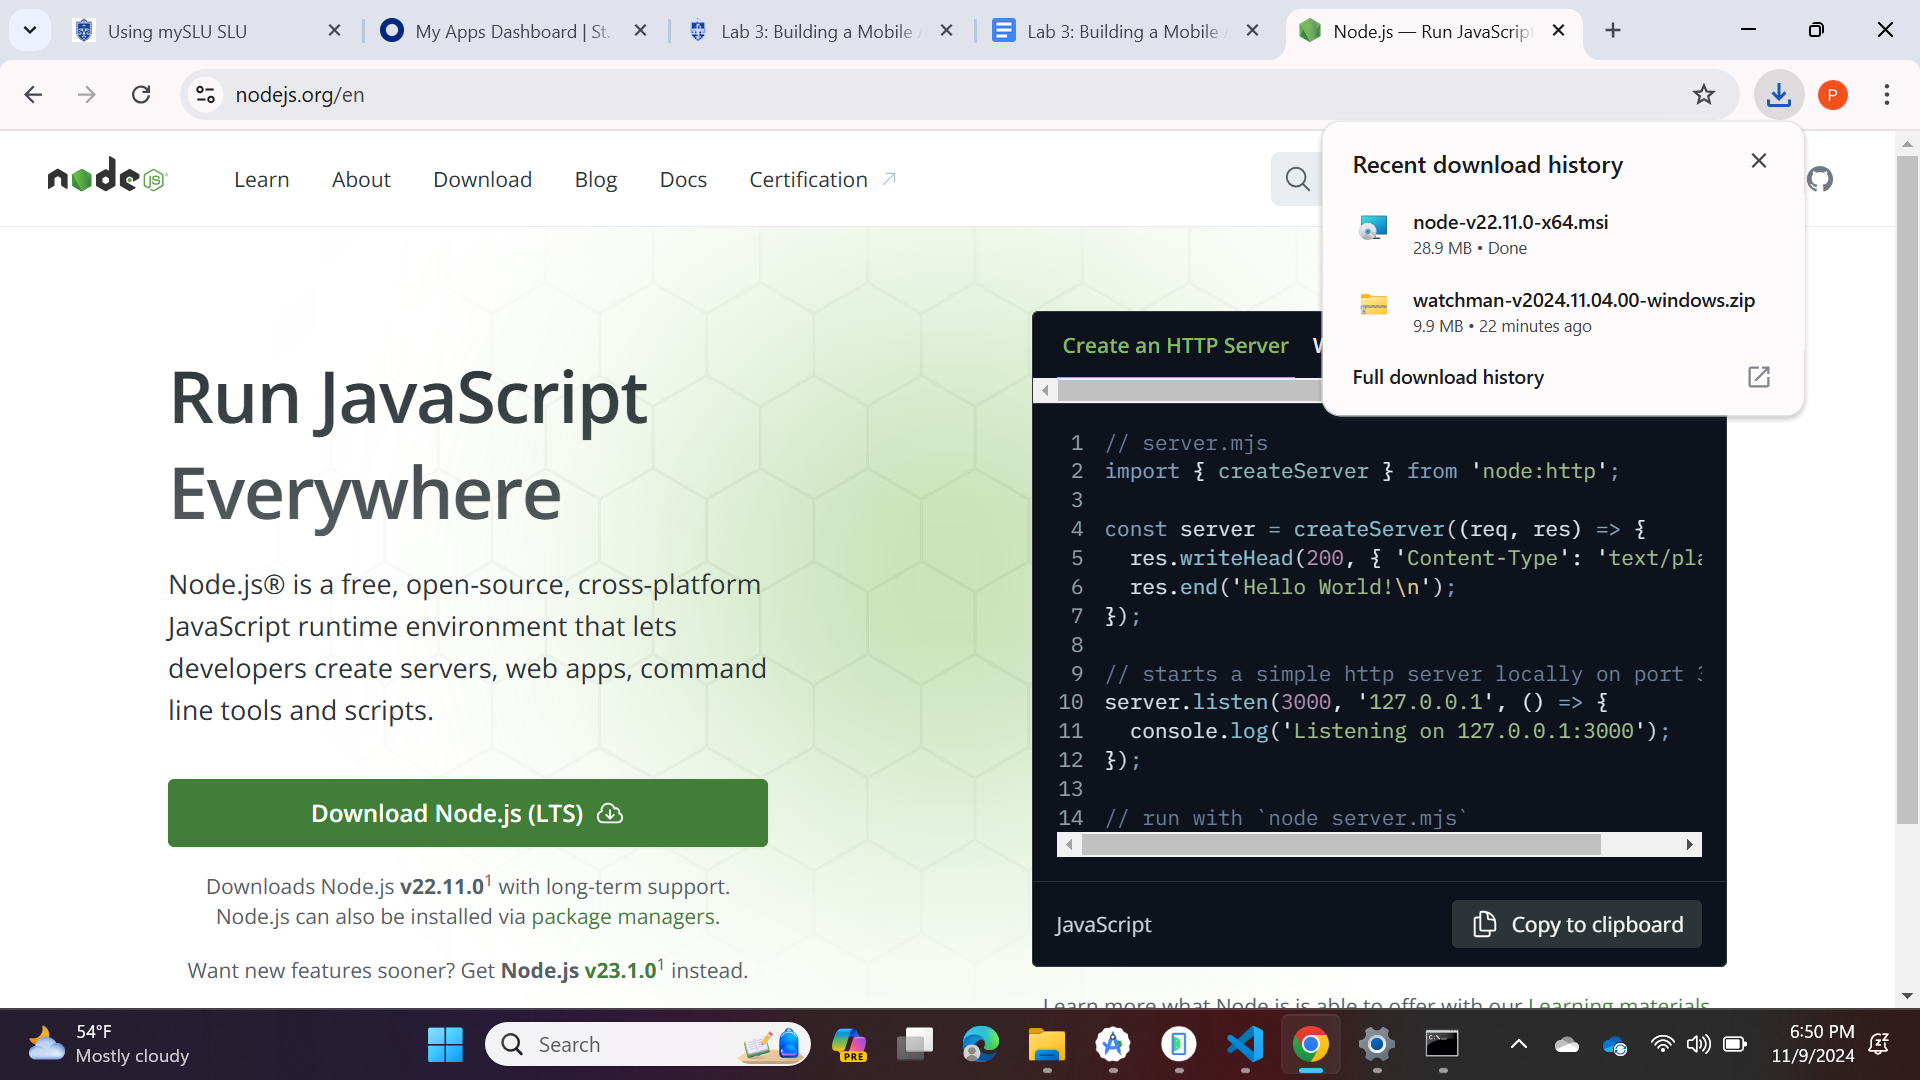
\includegraphics[width=5.57813in,height=3.13391in]{media/image2.png}
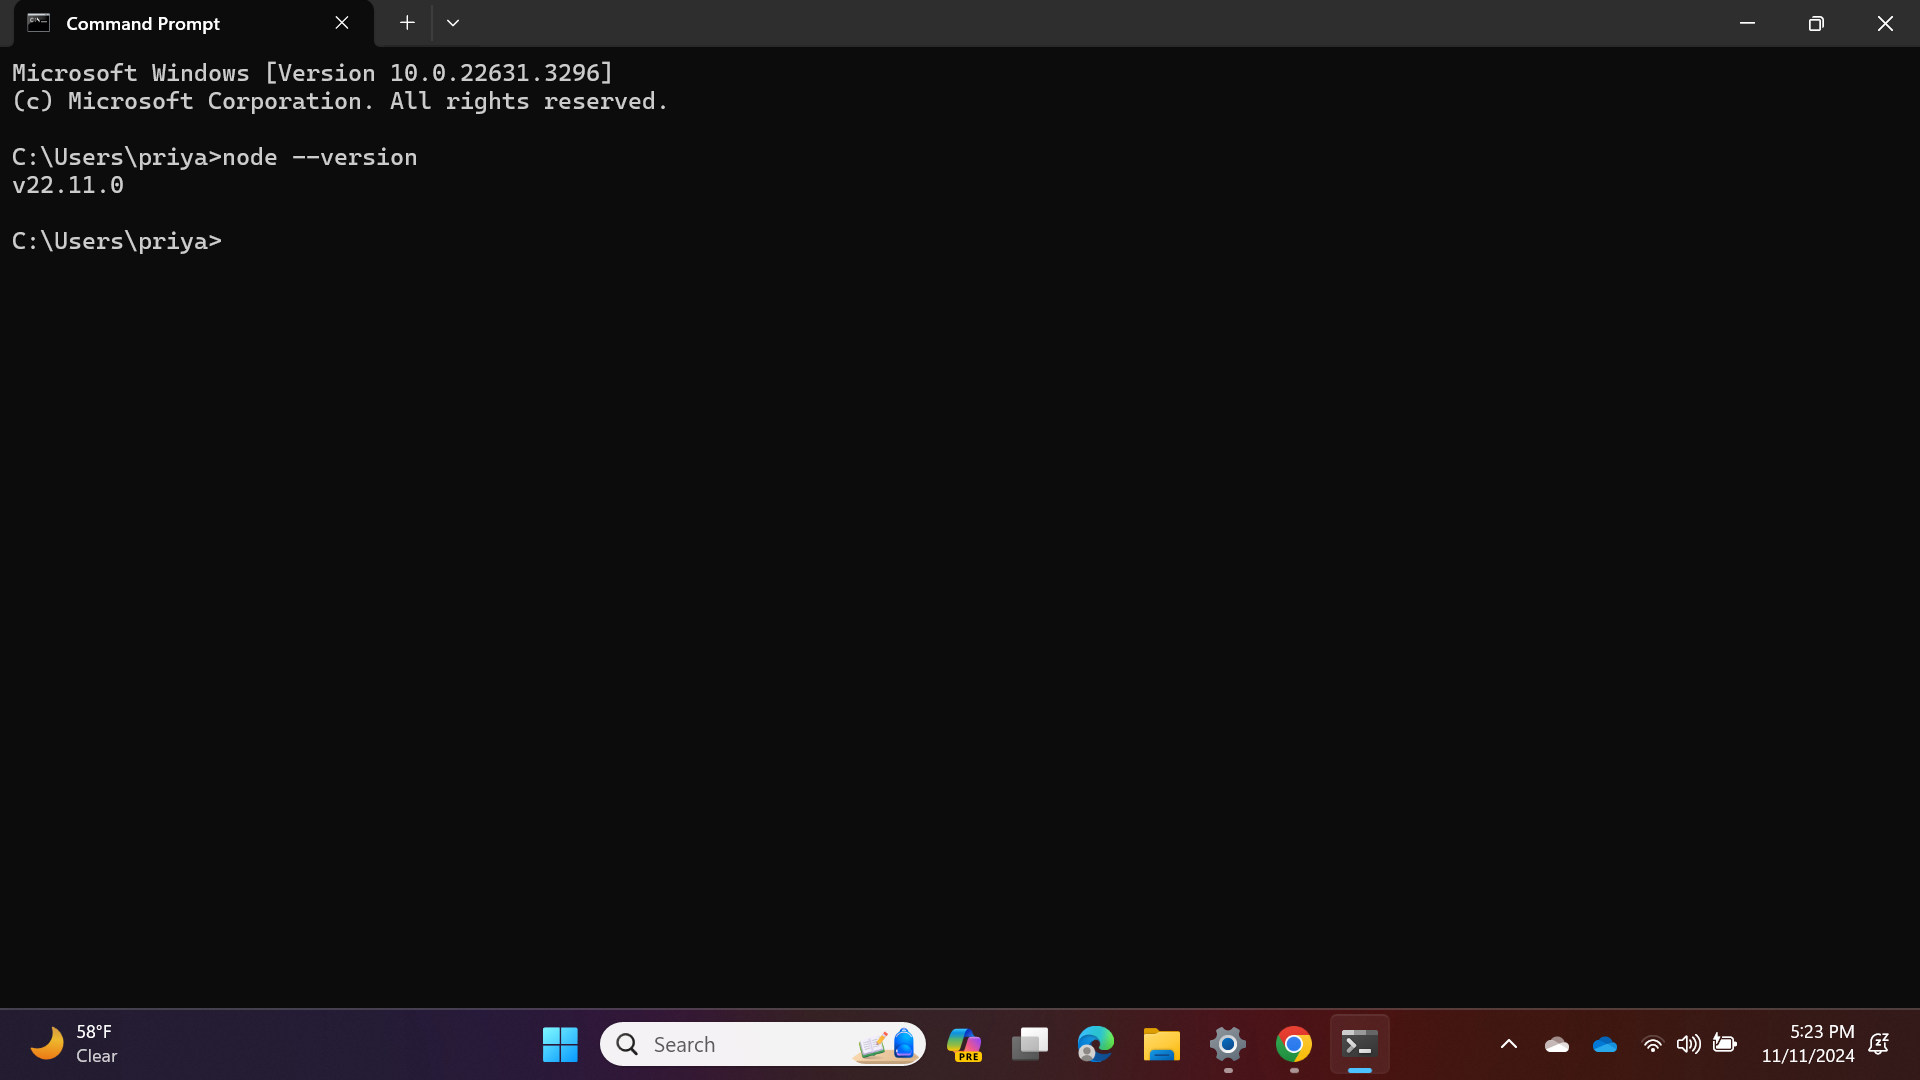
\includegraphics[width=5.57813in,height=3.13391in]{media/image9.png}
    
\begin{itemize}
    \item \textbf{Install Watchman (Optional for macOS/Linux):} 
\end{itemize}
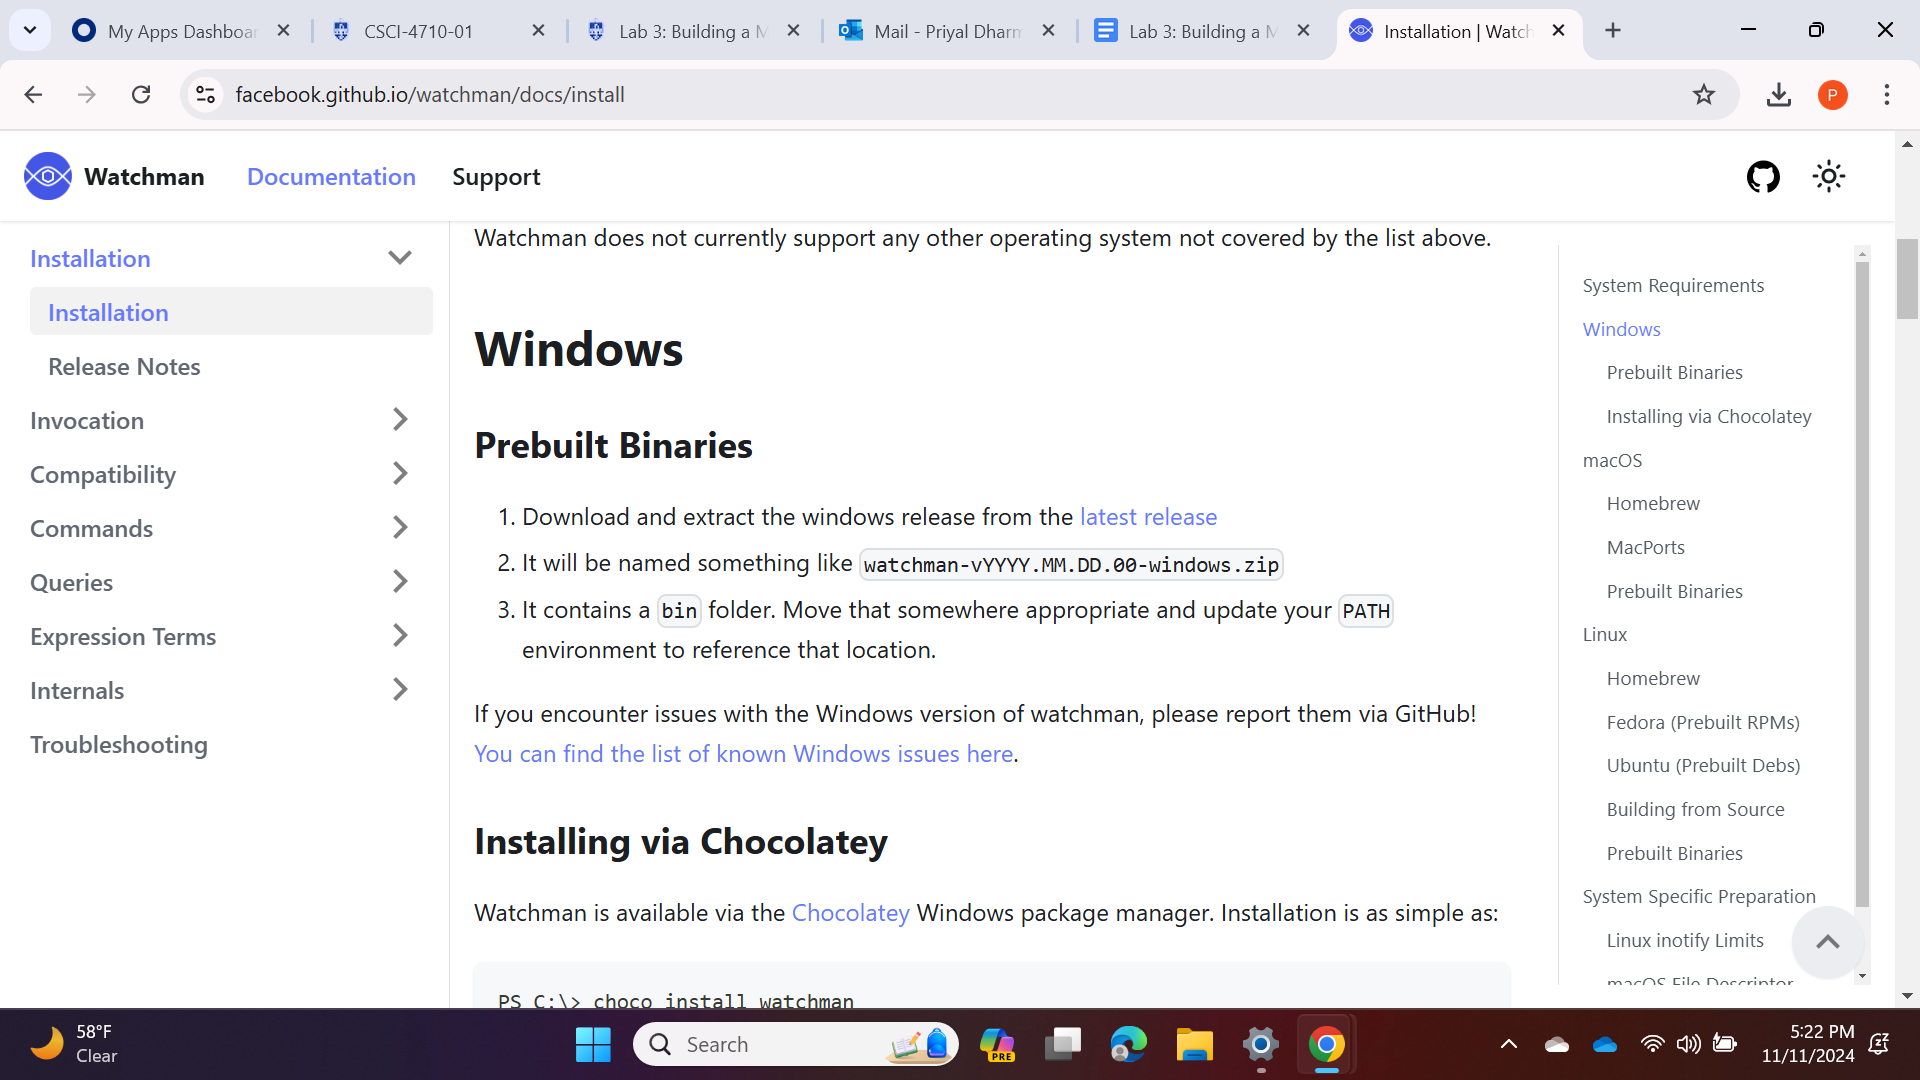
\includegraphics[width=5.57813in,height=3.13391in]{media/image1.png}
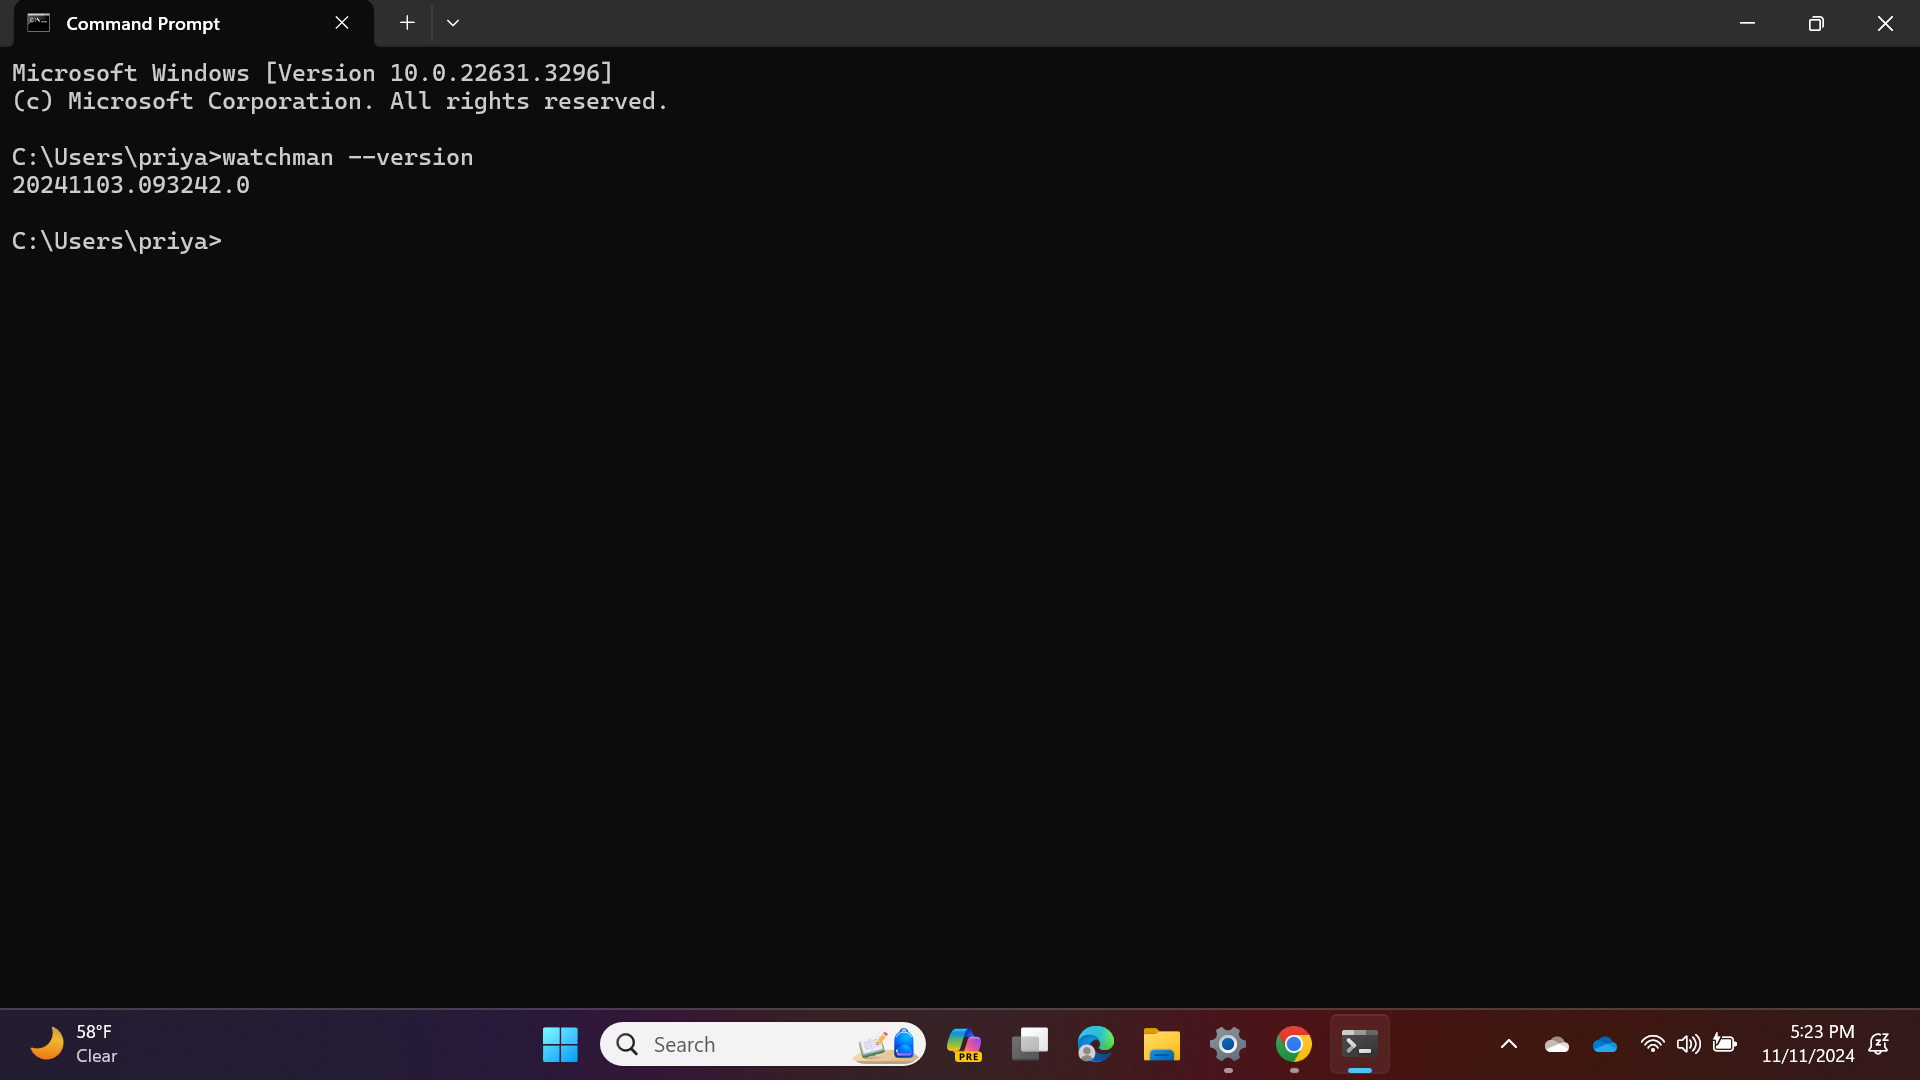
\includegraphics[width=5.57813in,height=3.13391in]{media/image27.png}


\subsection*{Step 2: Install React Native CLI}

The React Native CLI allows you to create and manage React Native projects.

\begin{itemize}
    \item Open your terminal and run:
    \begin{lstlisting}
    npm install -g react-native-cli
    \end{lstlisting}
\end{itemize}
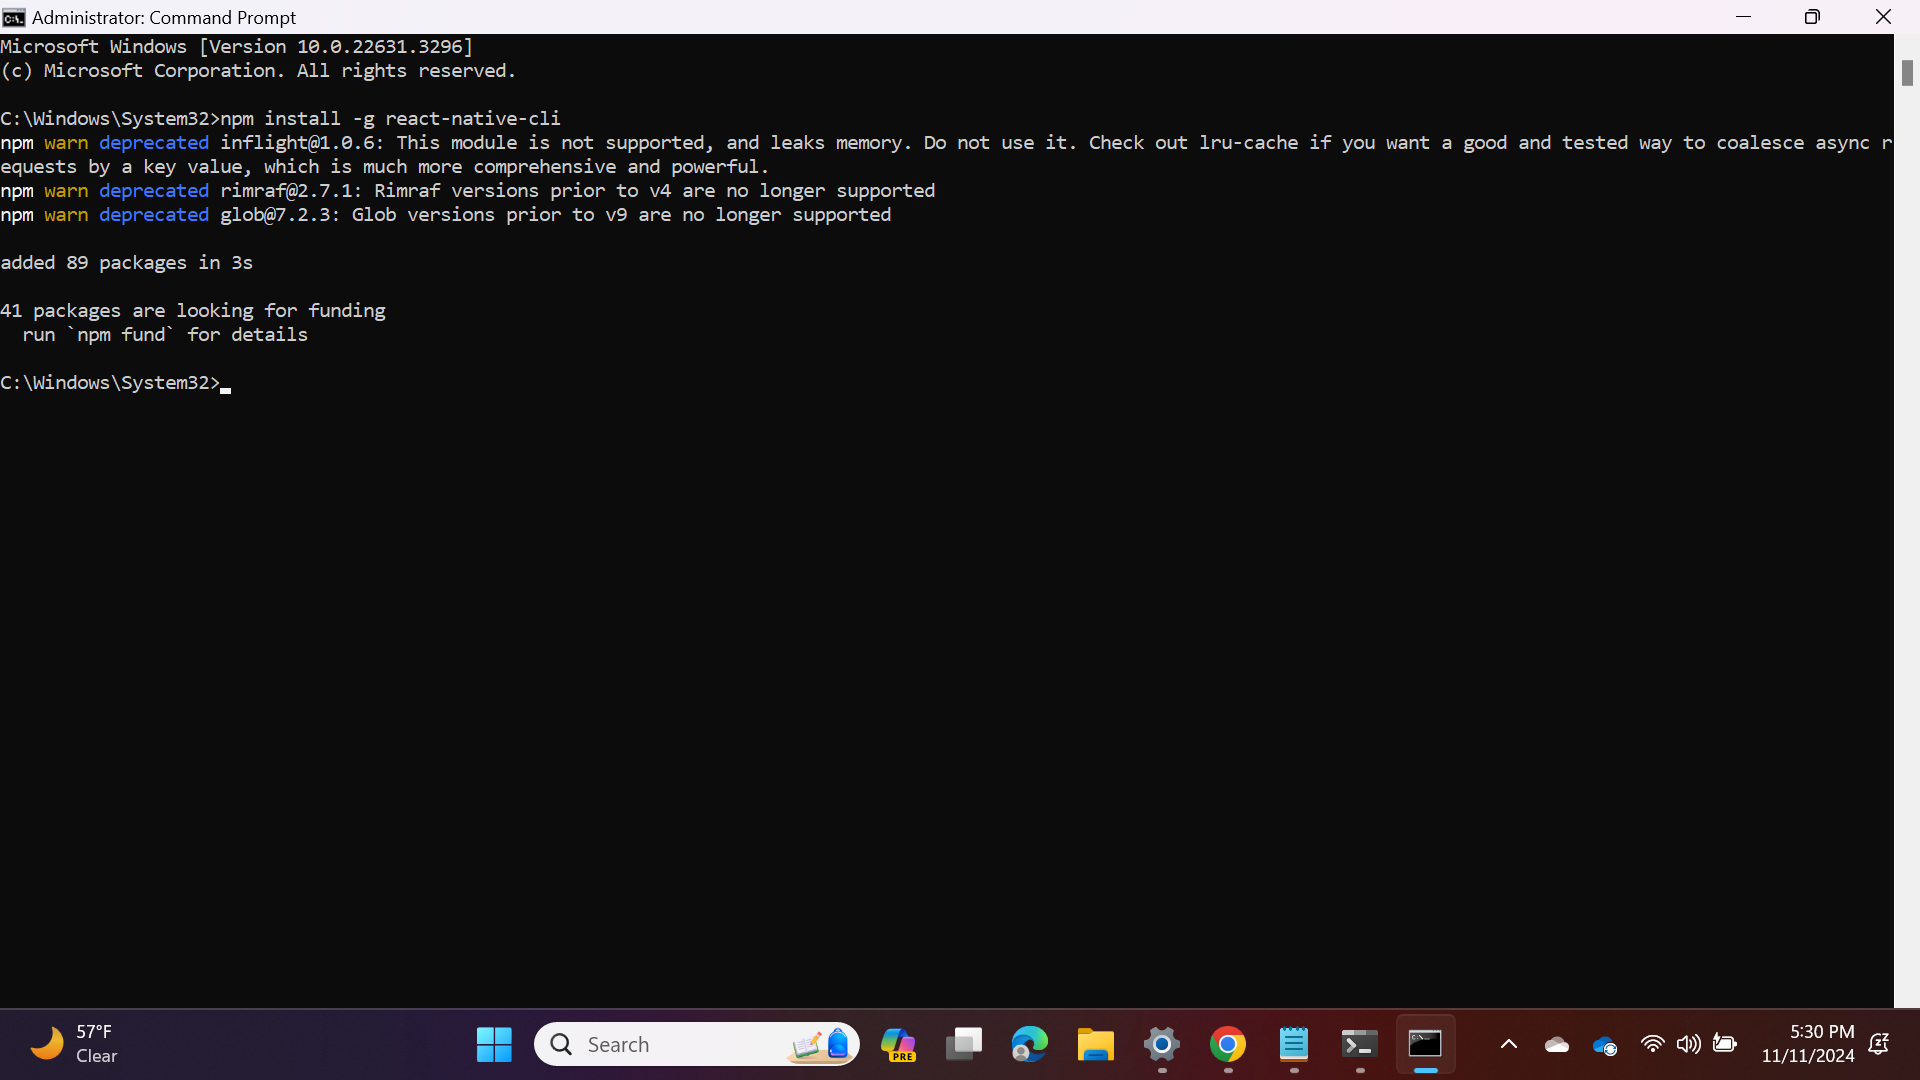
\includegraphics[width=5.57813in,height=3.13391in]{media/image33.png}

\begin{itemize}
    \item If the global package is deprecated, use the local version with:
    \begin{lstlisting}
    npx react-native init YourProjectName
    \end{lstlisting}
\end{itemize}
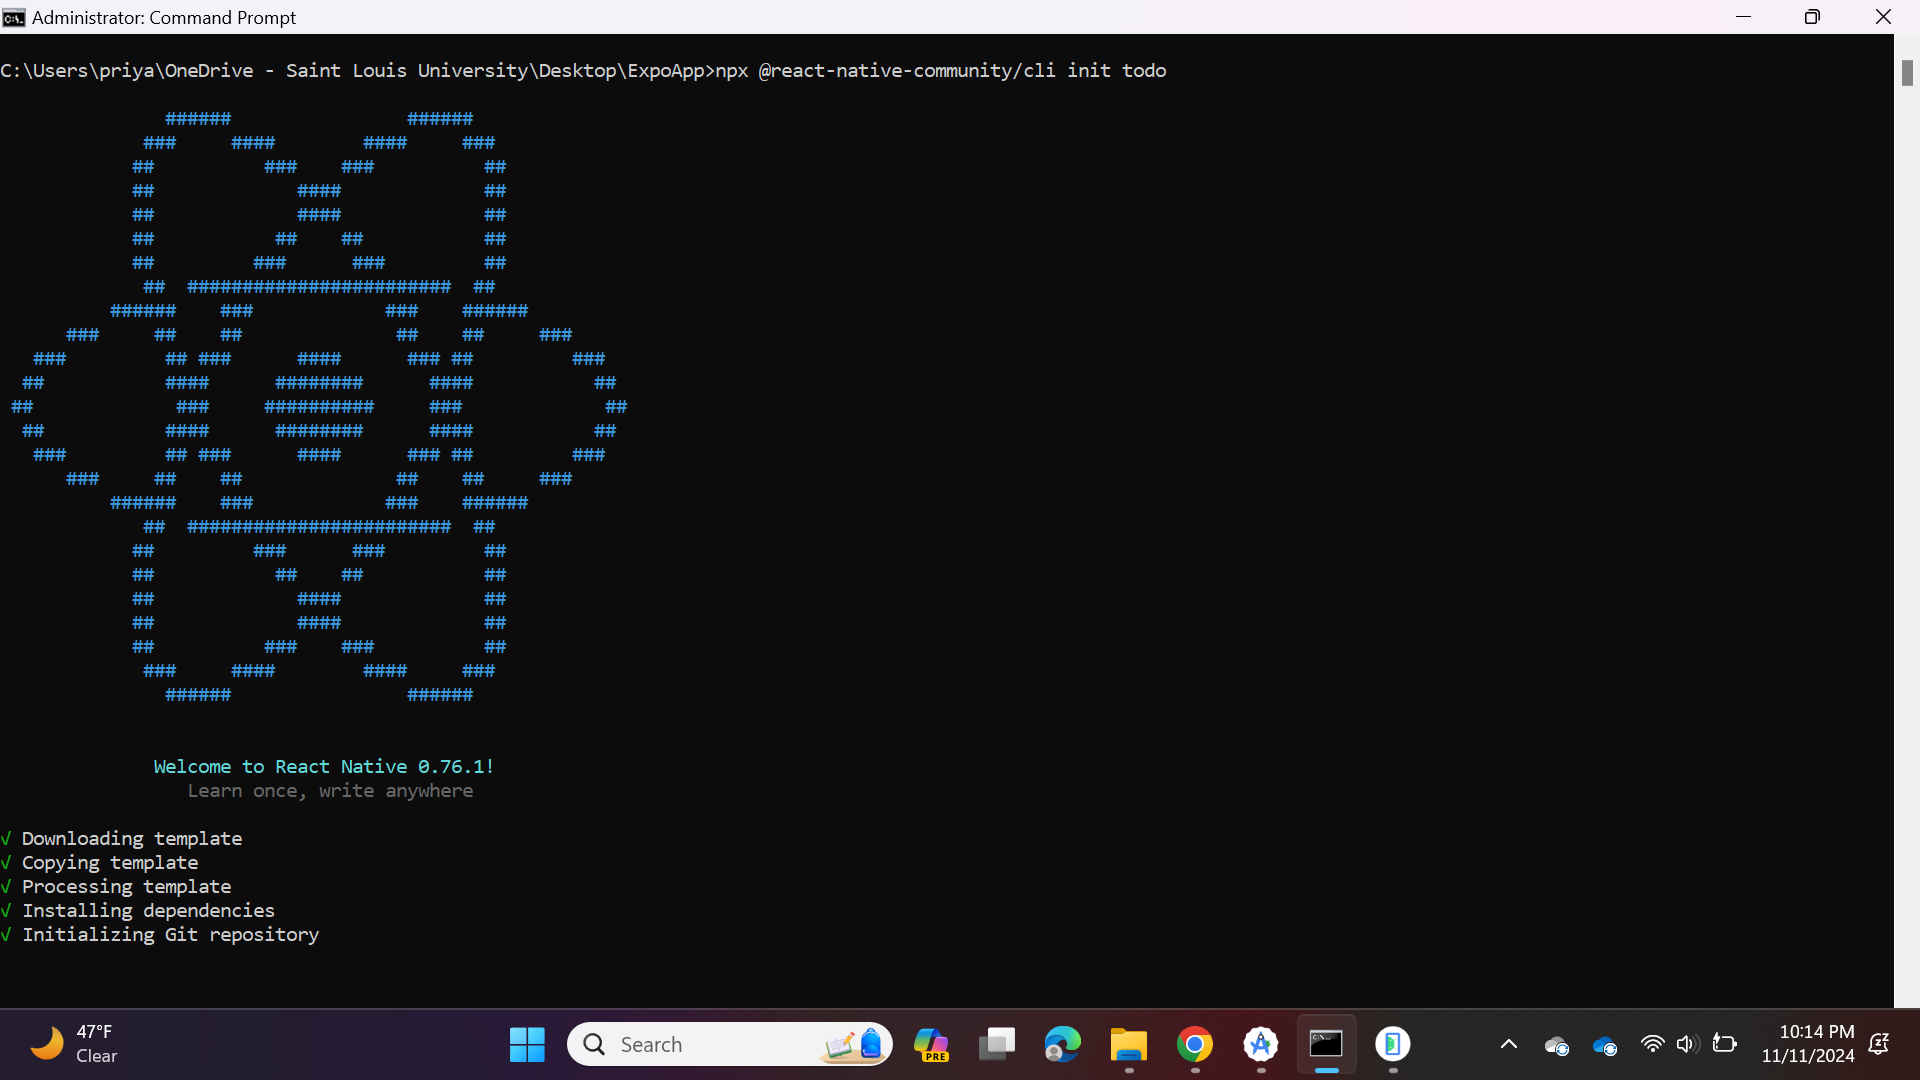
\includegraphics[width=5.57813in,height=3.13391in]{media/image10.png}
    


\subsection*{Step 3: Set Up Android Studio (or Xcode for iOS)}

\textbf{For Android Users:}
\begin{enumerate}
    \item Download and install Android Studio from  {https://developer.android.com/studio}.
\end{enumerate}
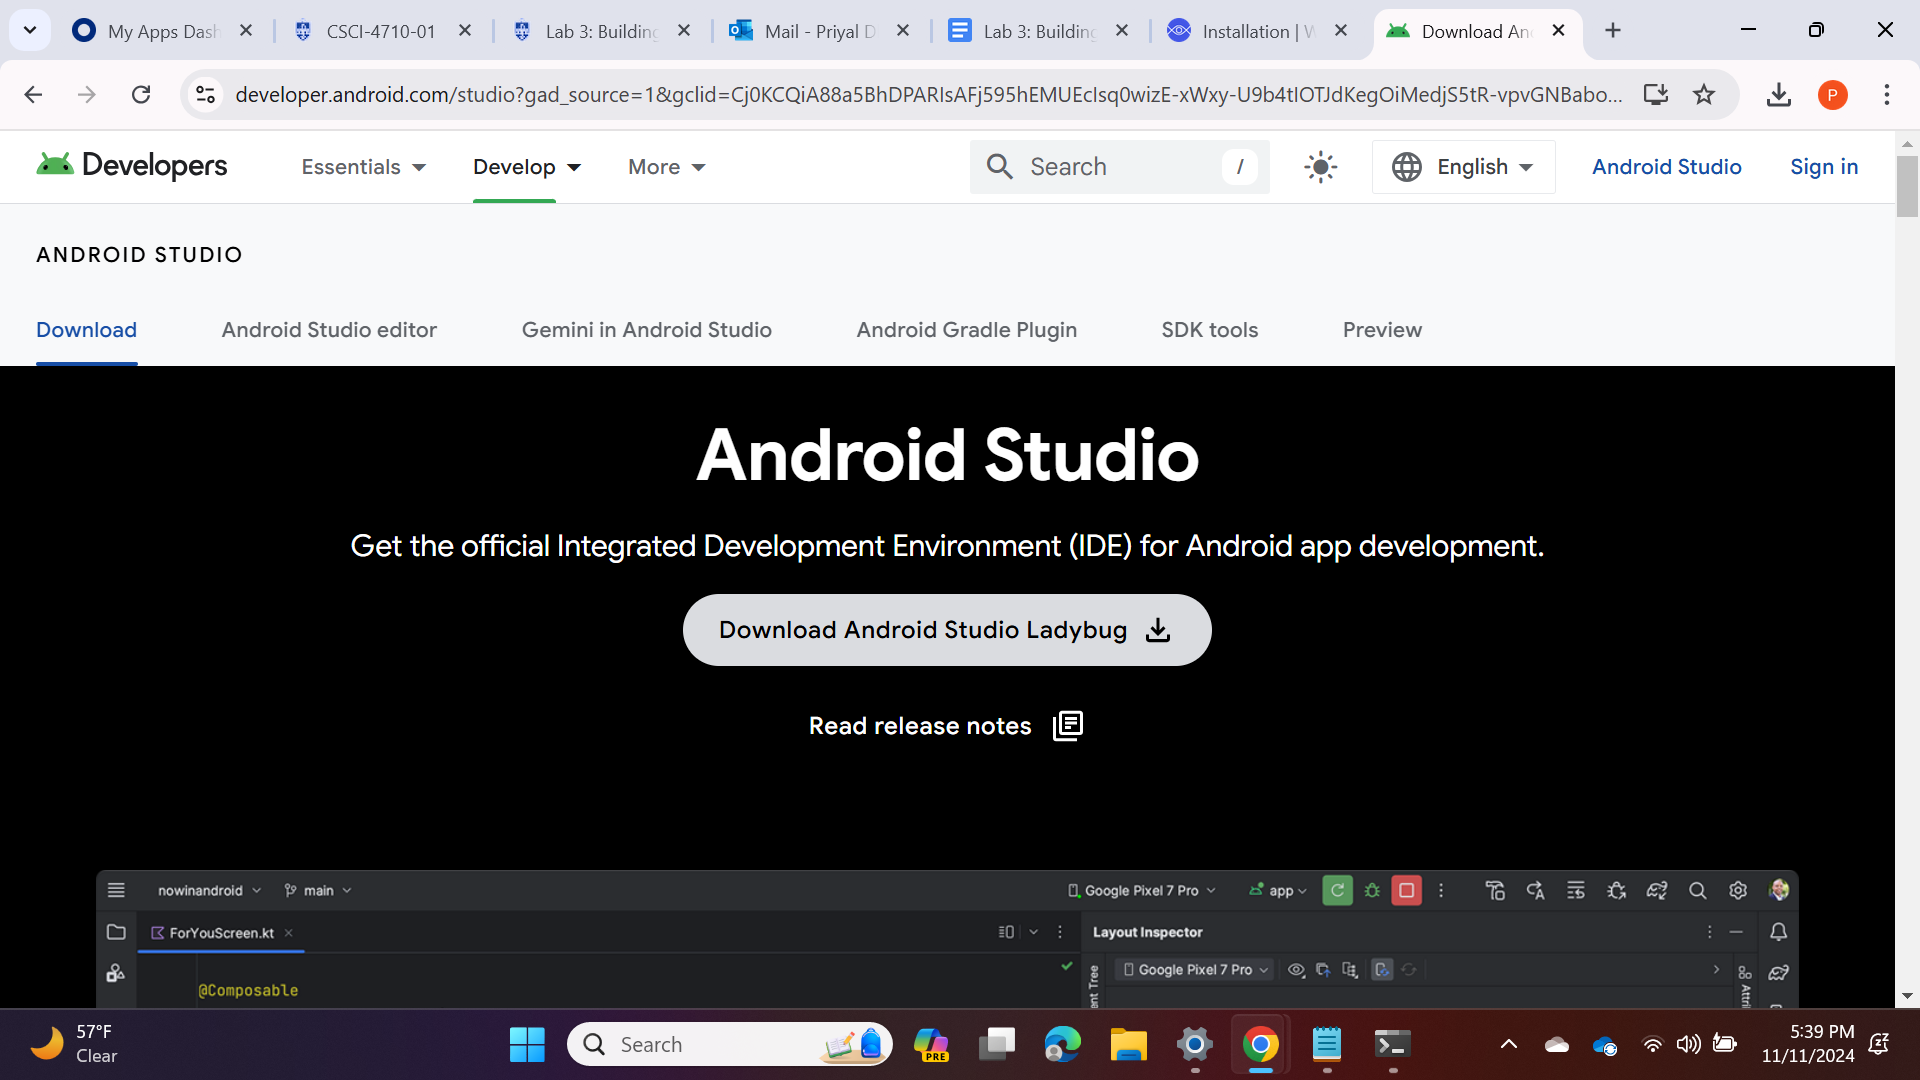
\includegraphics[width=5.57813in,height=3.13391in]{media/image26.png}
    
\begin{enumerate}
    \item Configure Android Studio:
    
        Preferences > Appearance \& Behavior > System Settings > Android SDK
\end{enumerate}
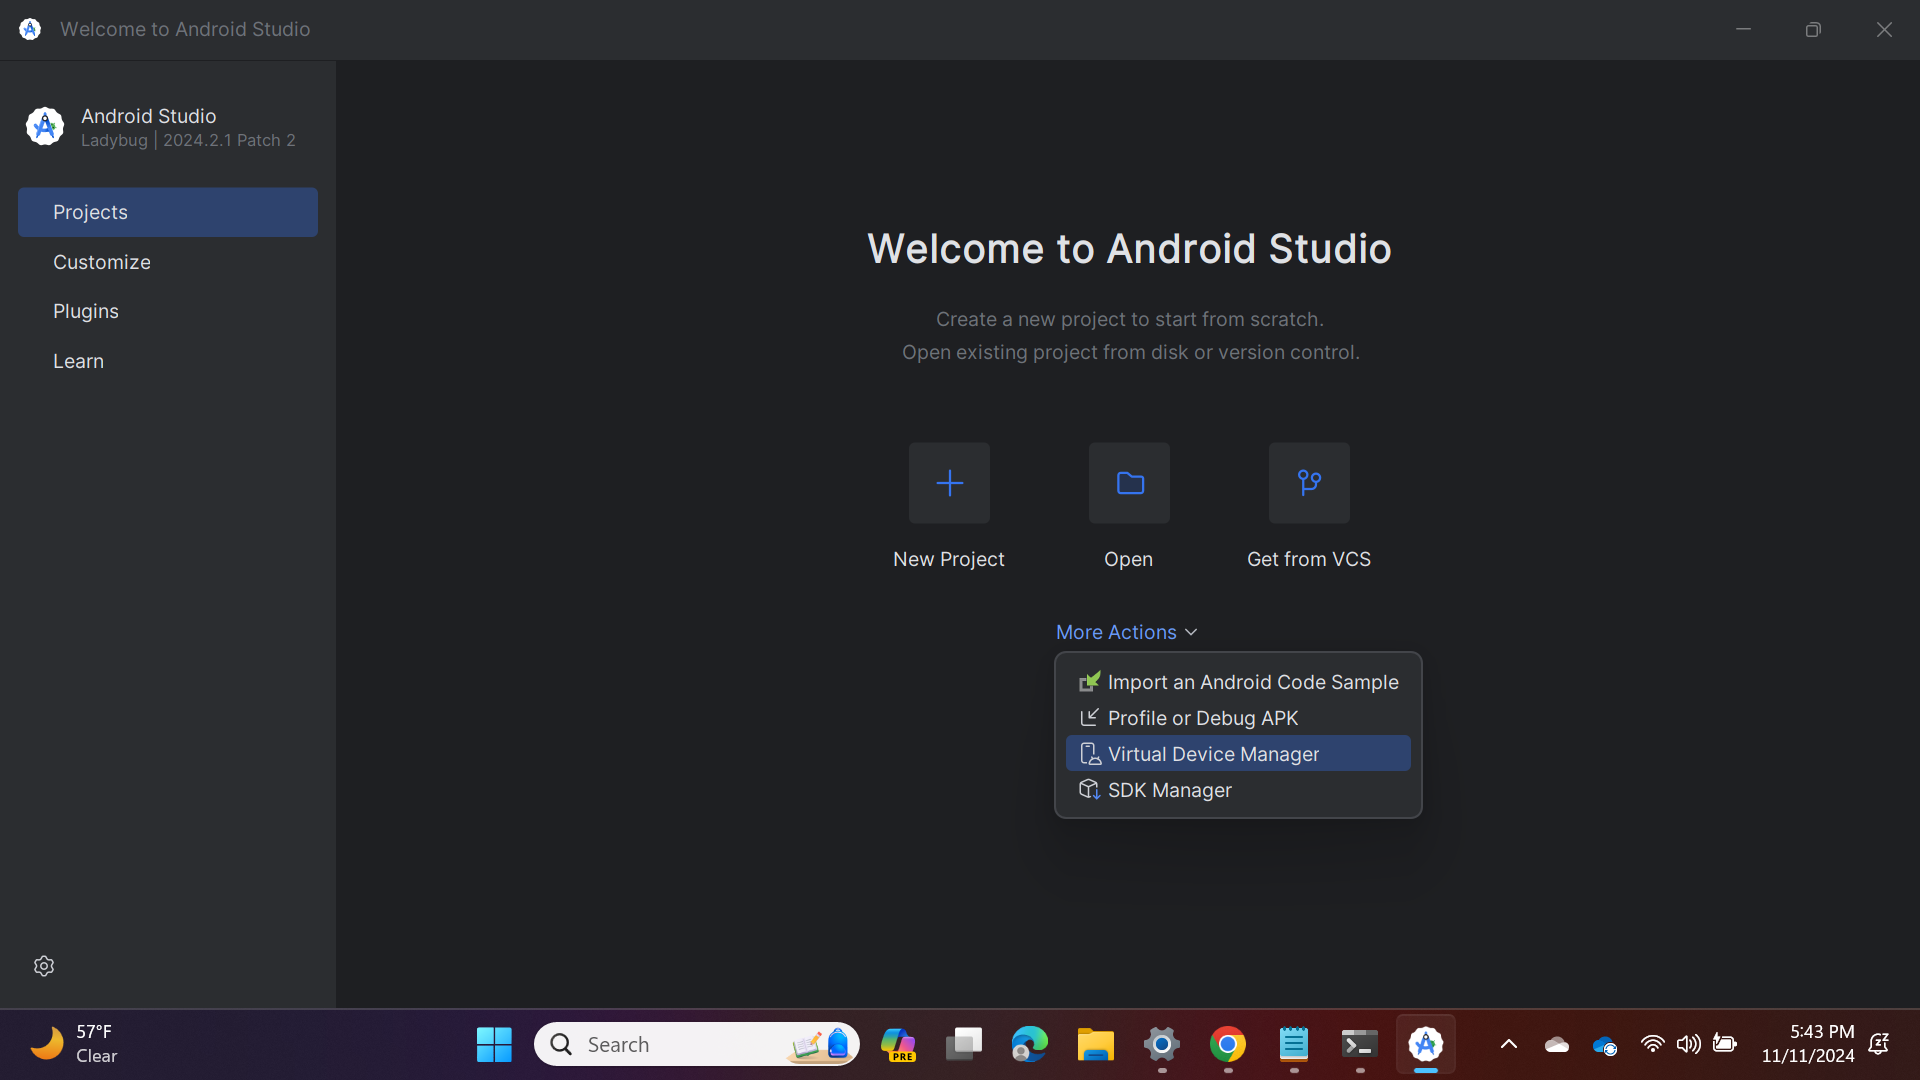
\includegraphics[width=5.57813in,height=3.13391in]{media/image24.png}
    
\begin{enumerate}
    \item Enable the following recommended SDK tools:
    \begin{itemize}
        \item Android SDK Build-Tools (latest version)
        \item Android SDK Platform-Tools
        \item Android Emulator
        \item Google Play Services (if required)
    \end{itemize}
\end{enumerate}
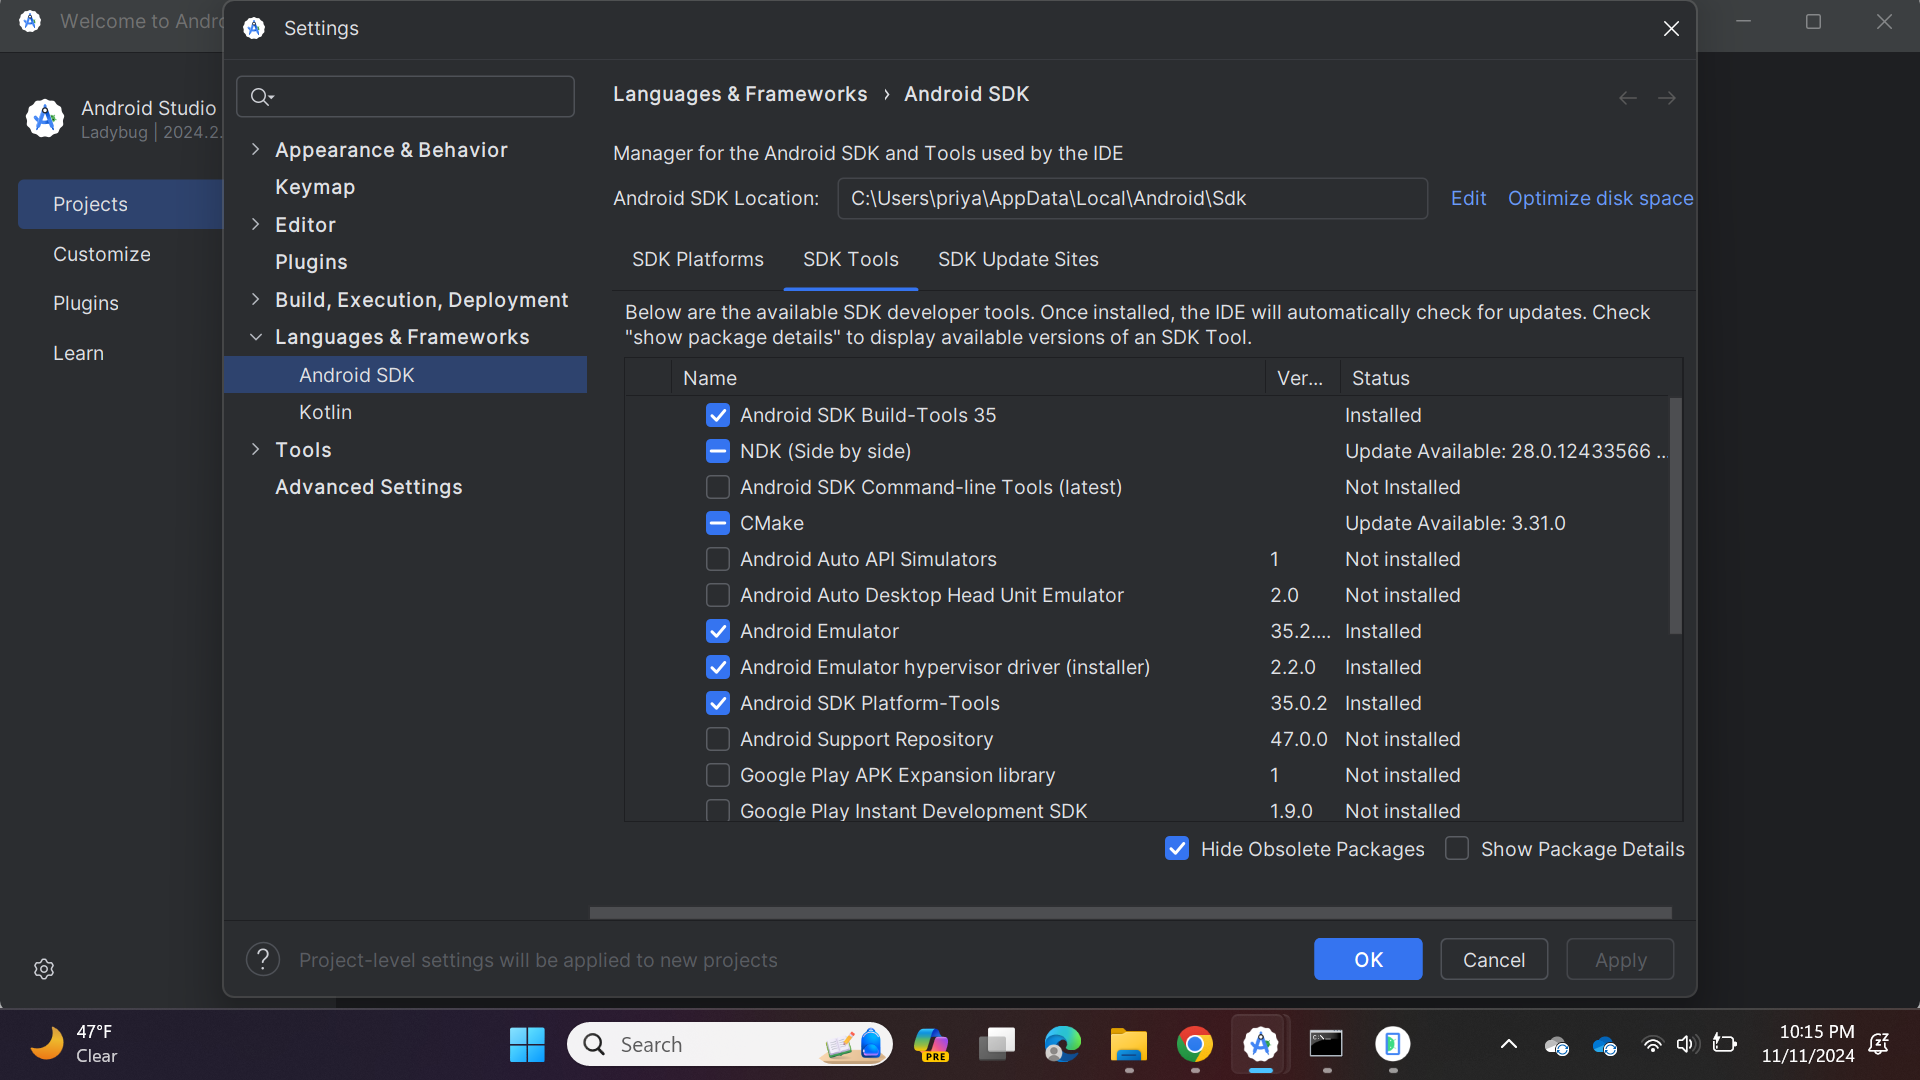
\includegraphics[width=5.57813in,height=3.13391in]{media/image31.png}
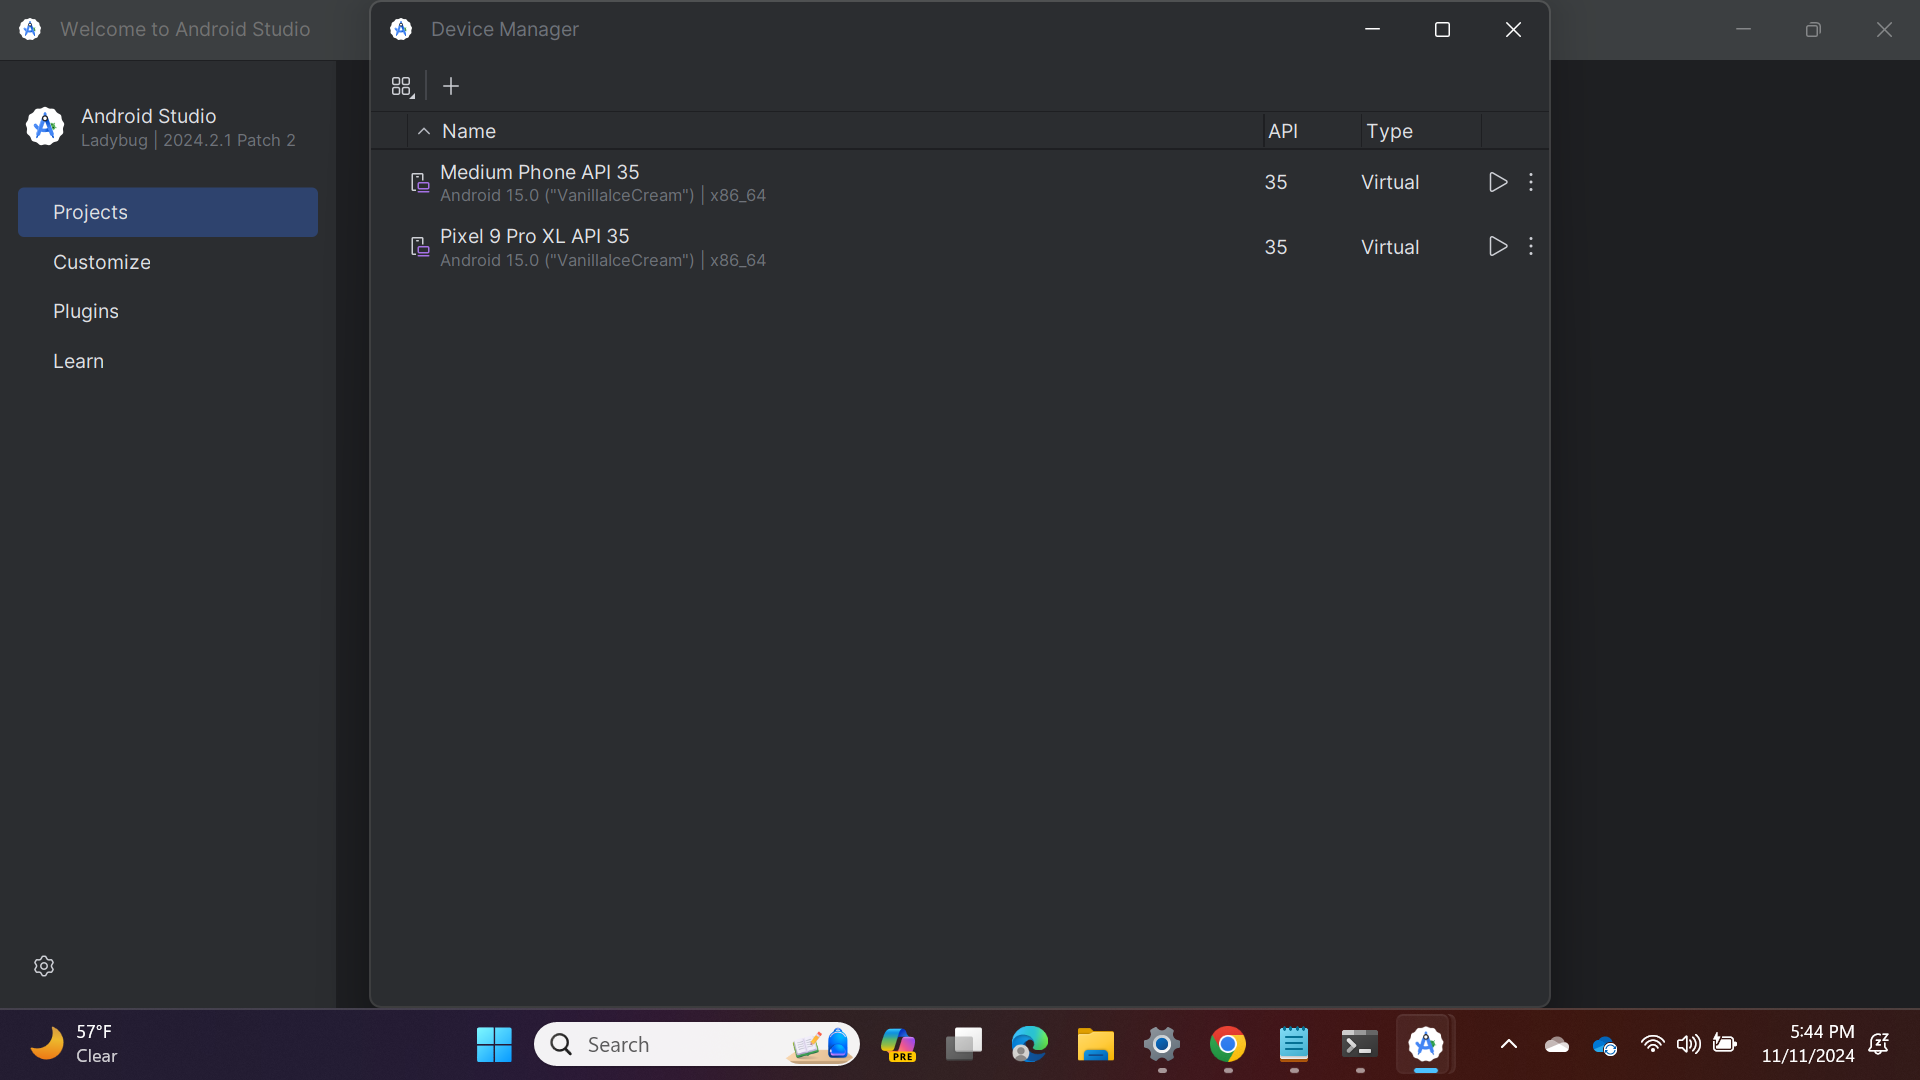
\includegraphics[width=5.57813in,height=3.13391in]{media/image22.png}
    
\subsection*{Step 4: Create a New React Native Project}

\begin{itemize}
    \item Run the following commands:
    \begin{lstlisting}[language=bash]
    npx react-native init YourProjectName
    cd YourProjectName
    \end{lstlisting}
    \item This creates a new React Native project.
\end{itemize}
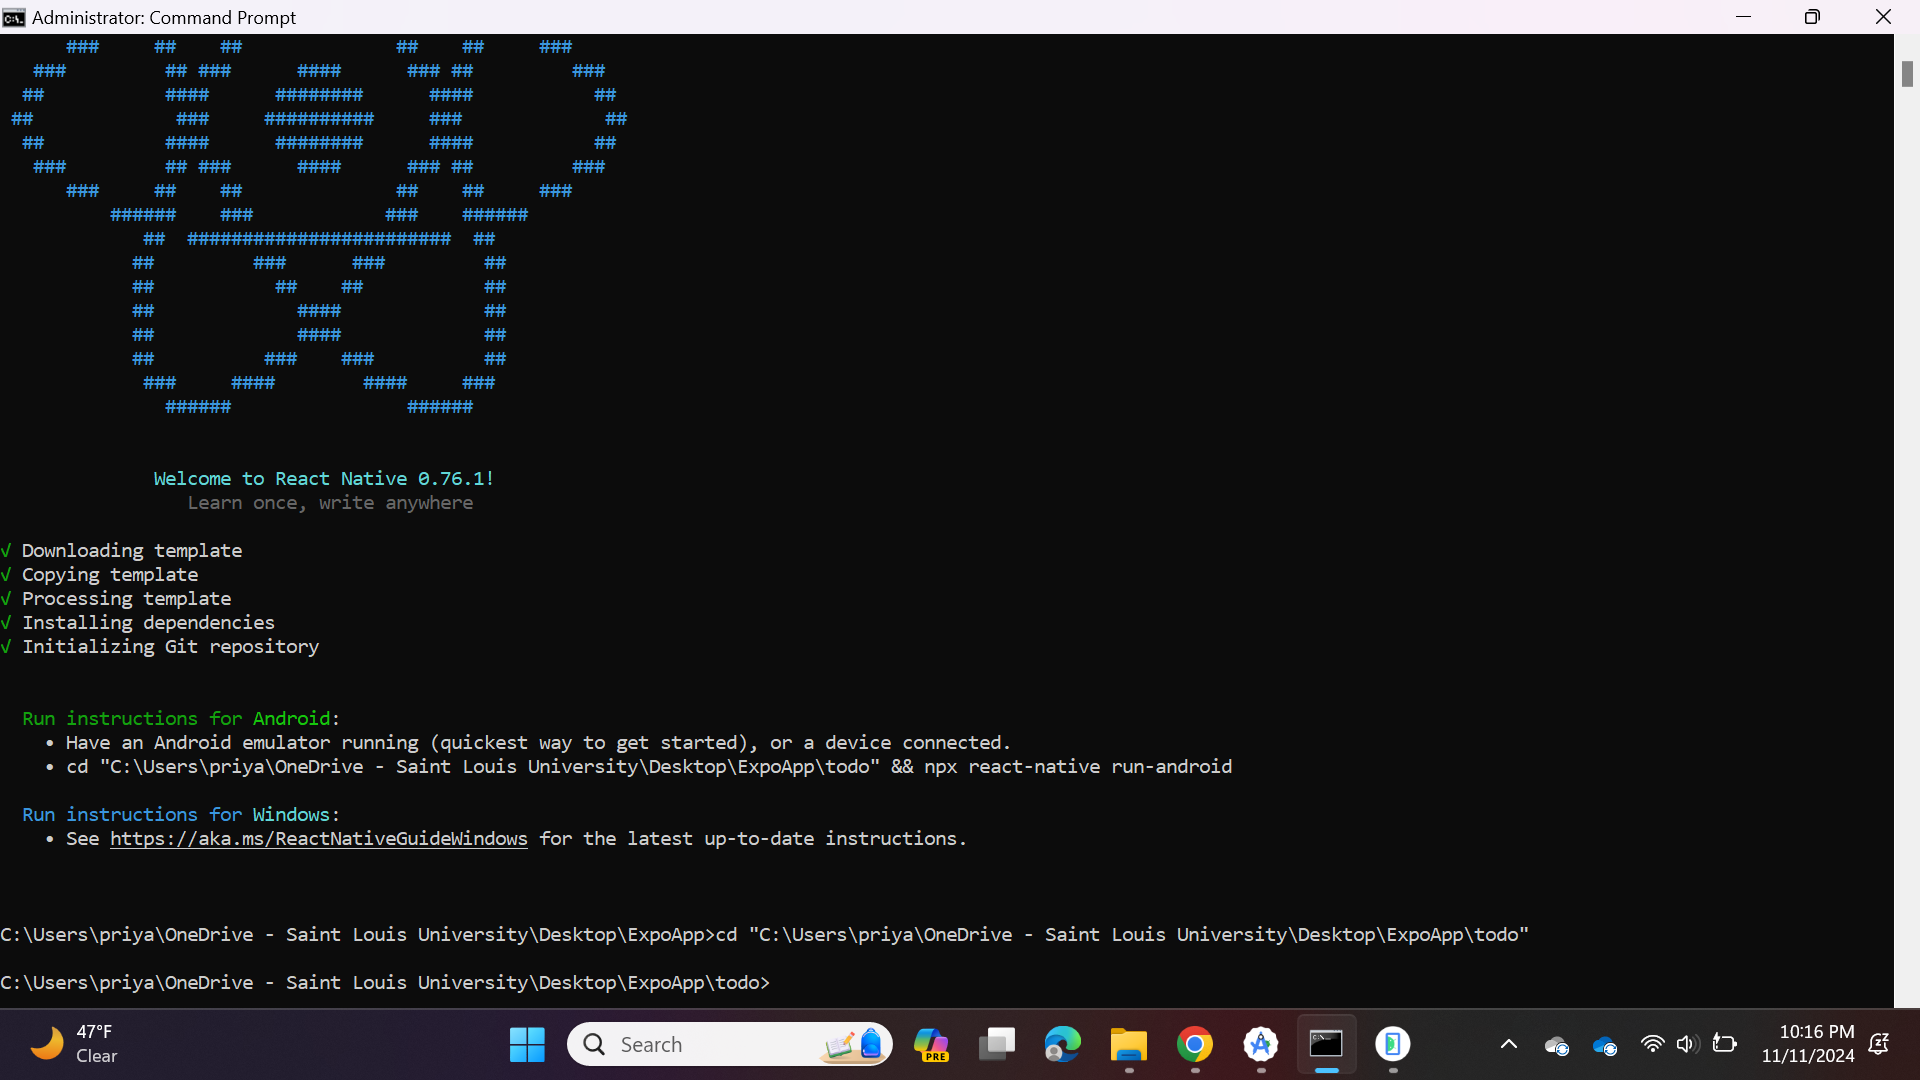
\includegraphics[width=5.57813in,height=3.13391in]{media/image18.png}

\subsection*{Step 5: Open the Project in Visual Studio Code}

\begin{itemize}
    \item Launch Visual Studio Code.
    \item Open the project folder via \textbf{File > Open Folder}.
    \item Install the React Native Tools extension for enhanced development experience.
\end{itemize}
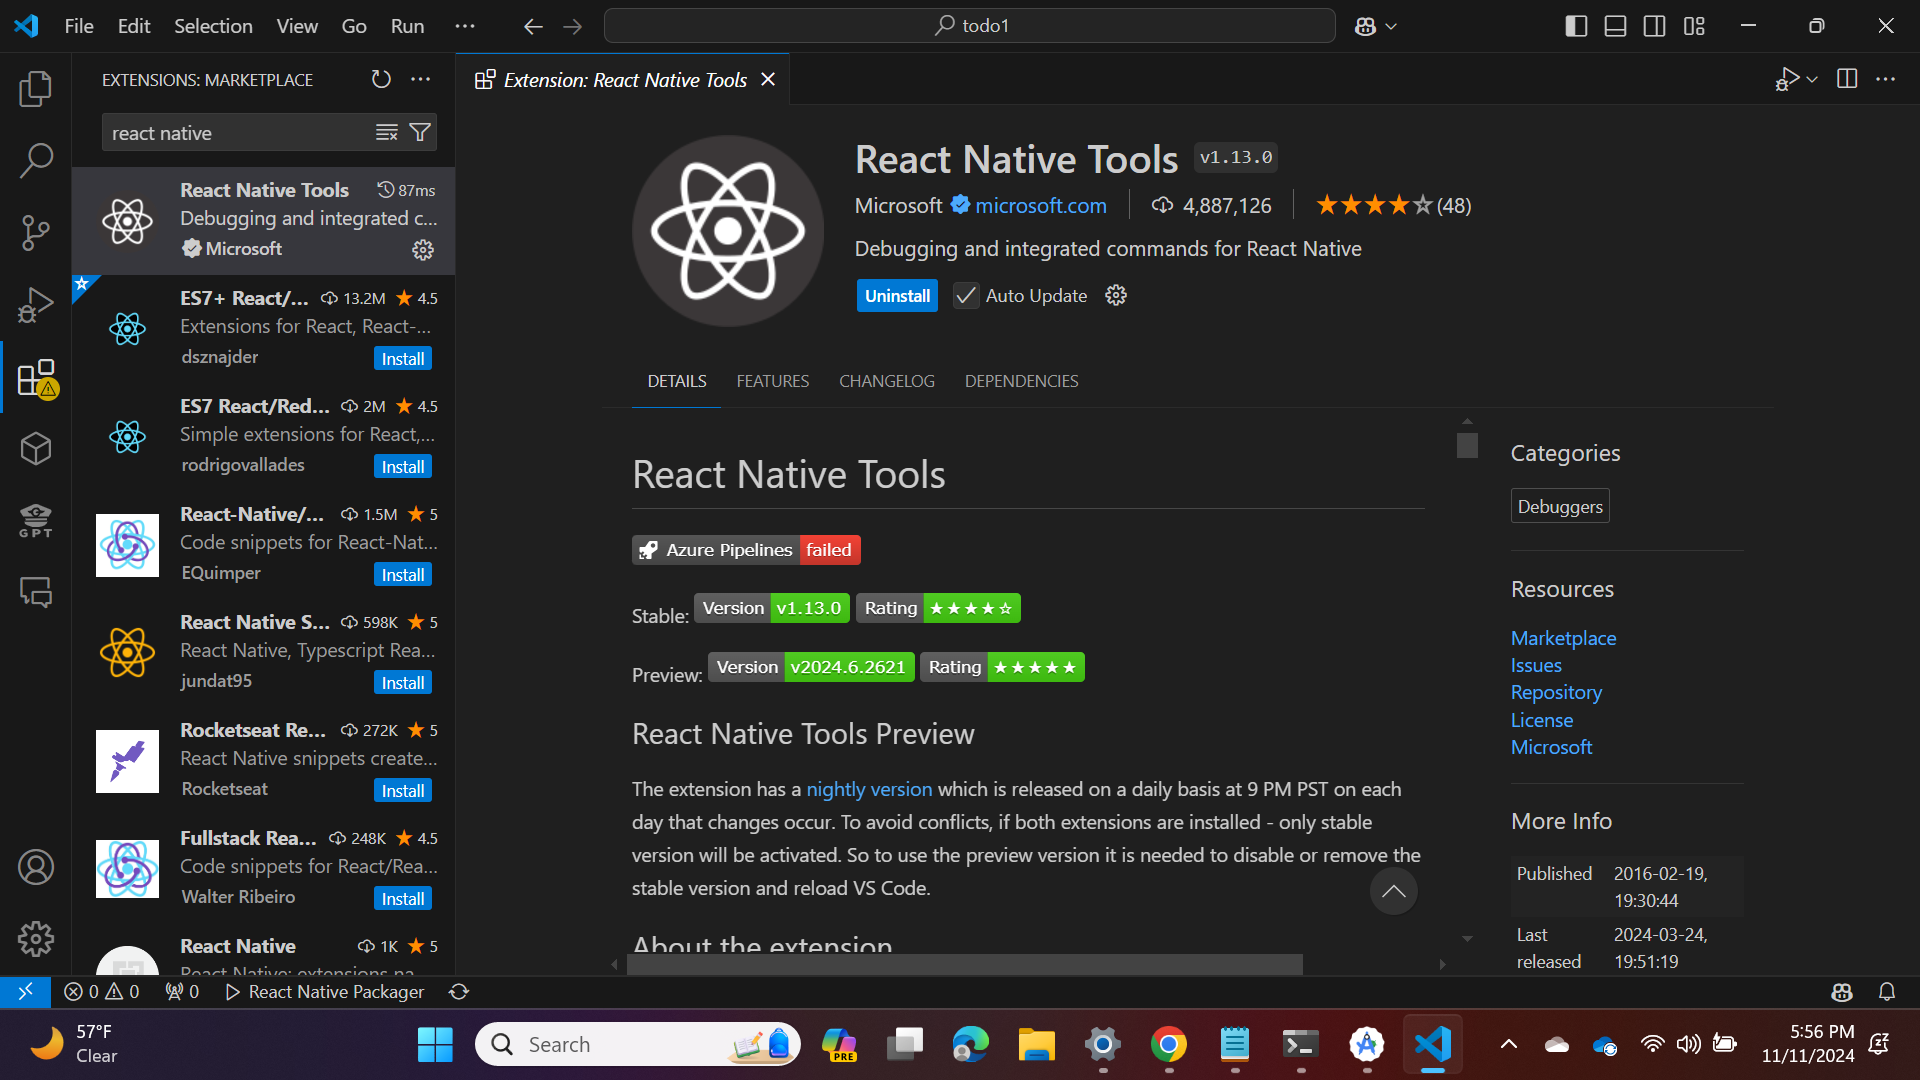
\includegraphics[width=5.57813in,height=3.13391in]{media/image15.png}

\begin{itemize} 
    \item Modify \texttt{App.js} to display \textit{"My First React Native Application"}.
\end{itemize}
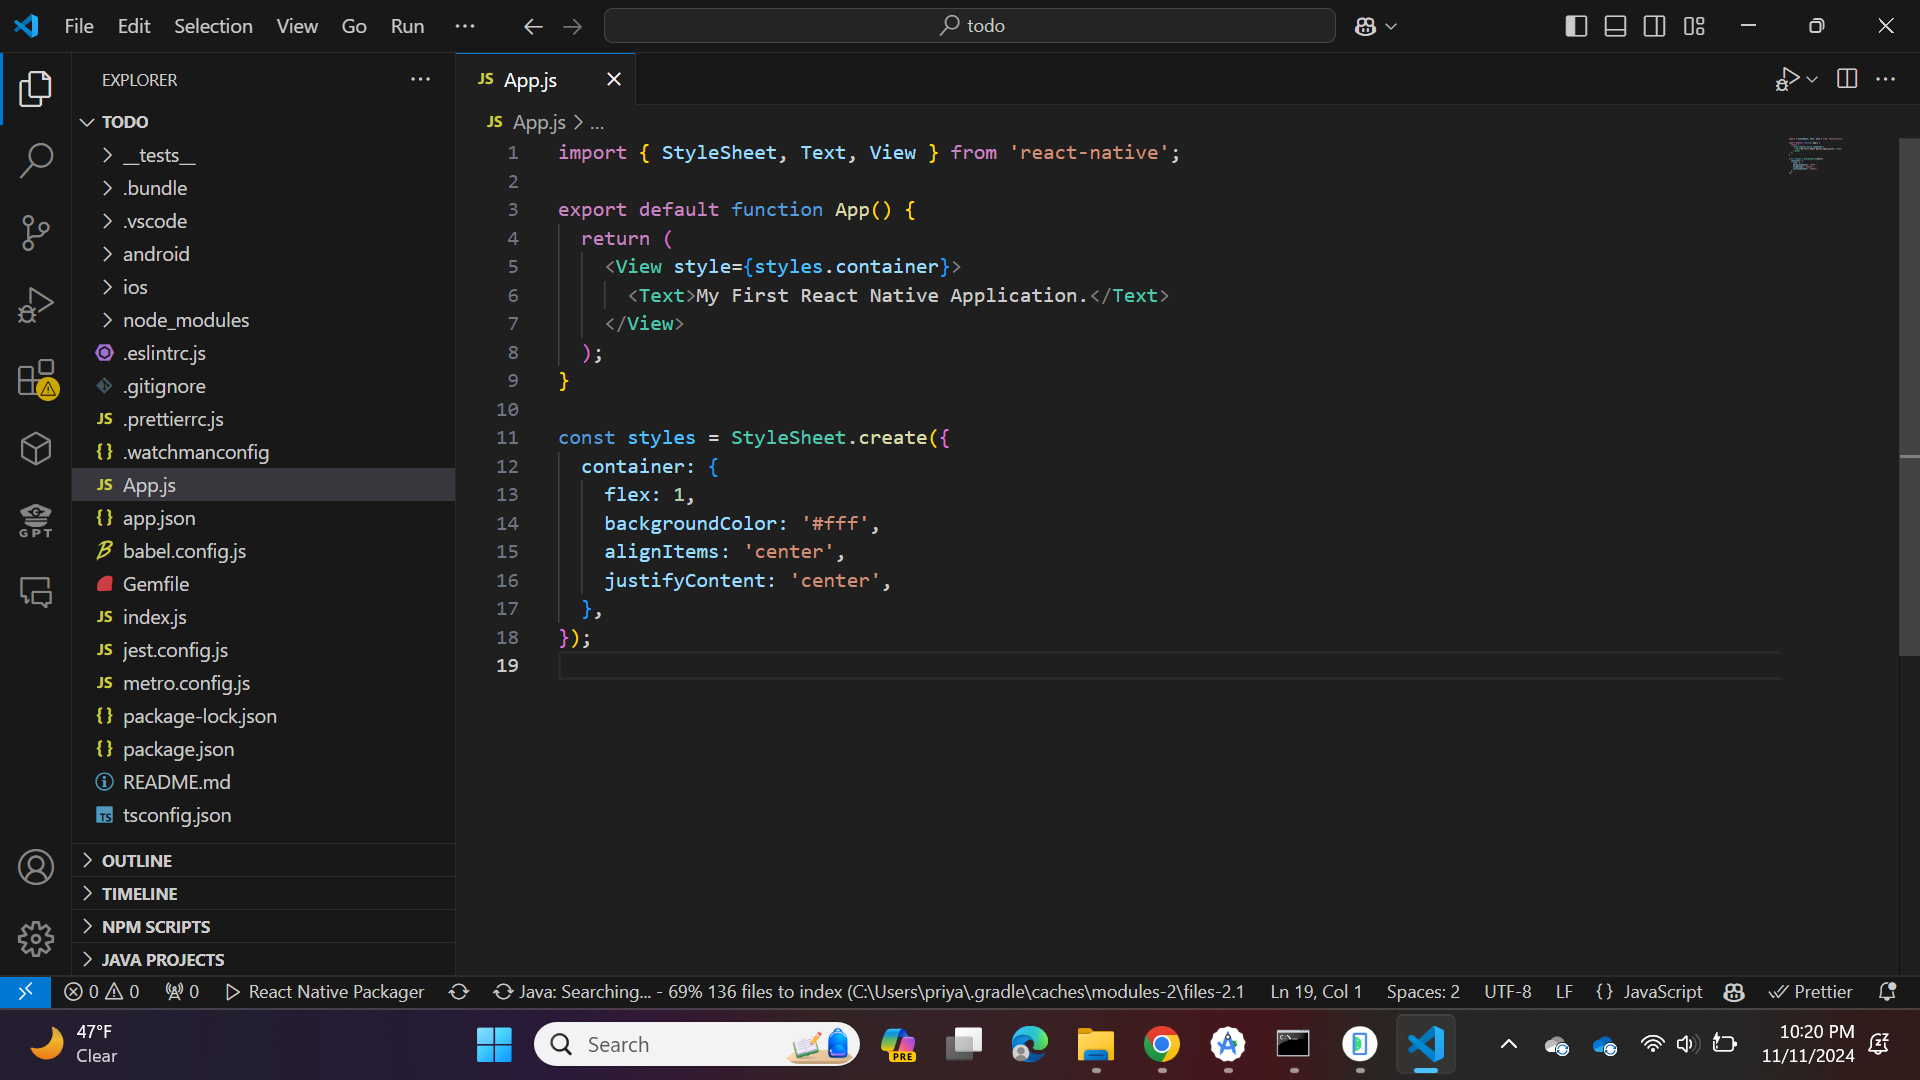
\includegraphics[width=5.57813in,height=3.13391in]{media/image29.png}

\subsection*{Step 6: Start the Metro Bundler}

\begin{itemize}
    \item Run the following command in the terminal:
    \begin{lstlisting}[language=bash]
    npx react-native start
    \end{lstlisting}
\end{itemize}
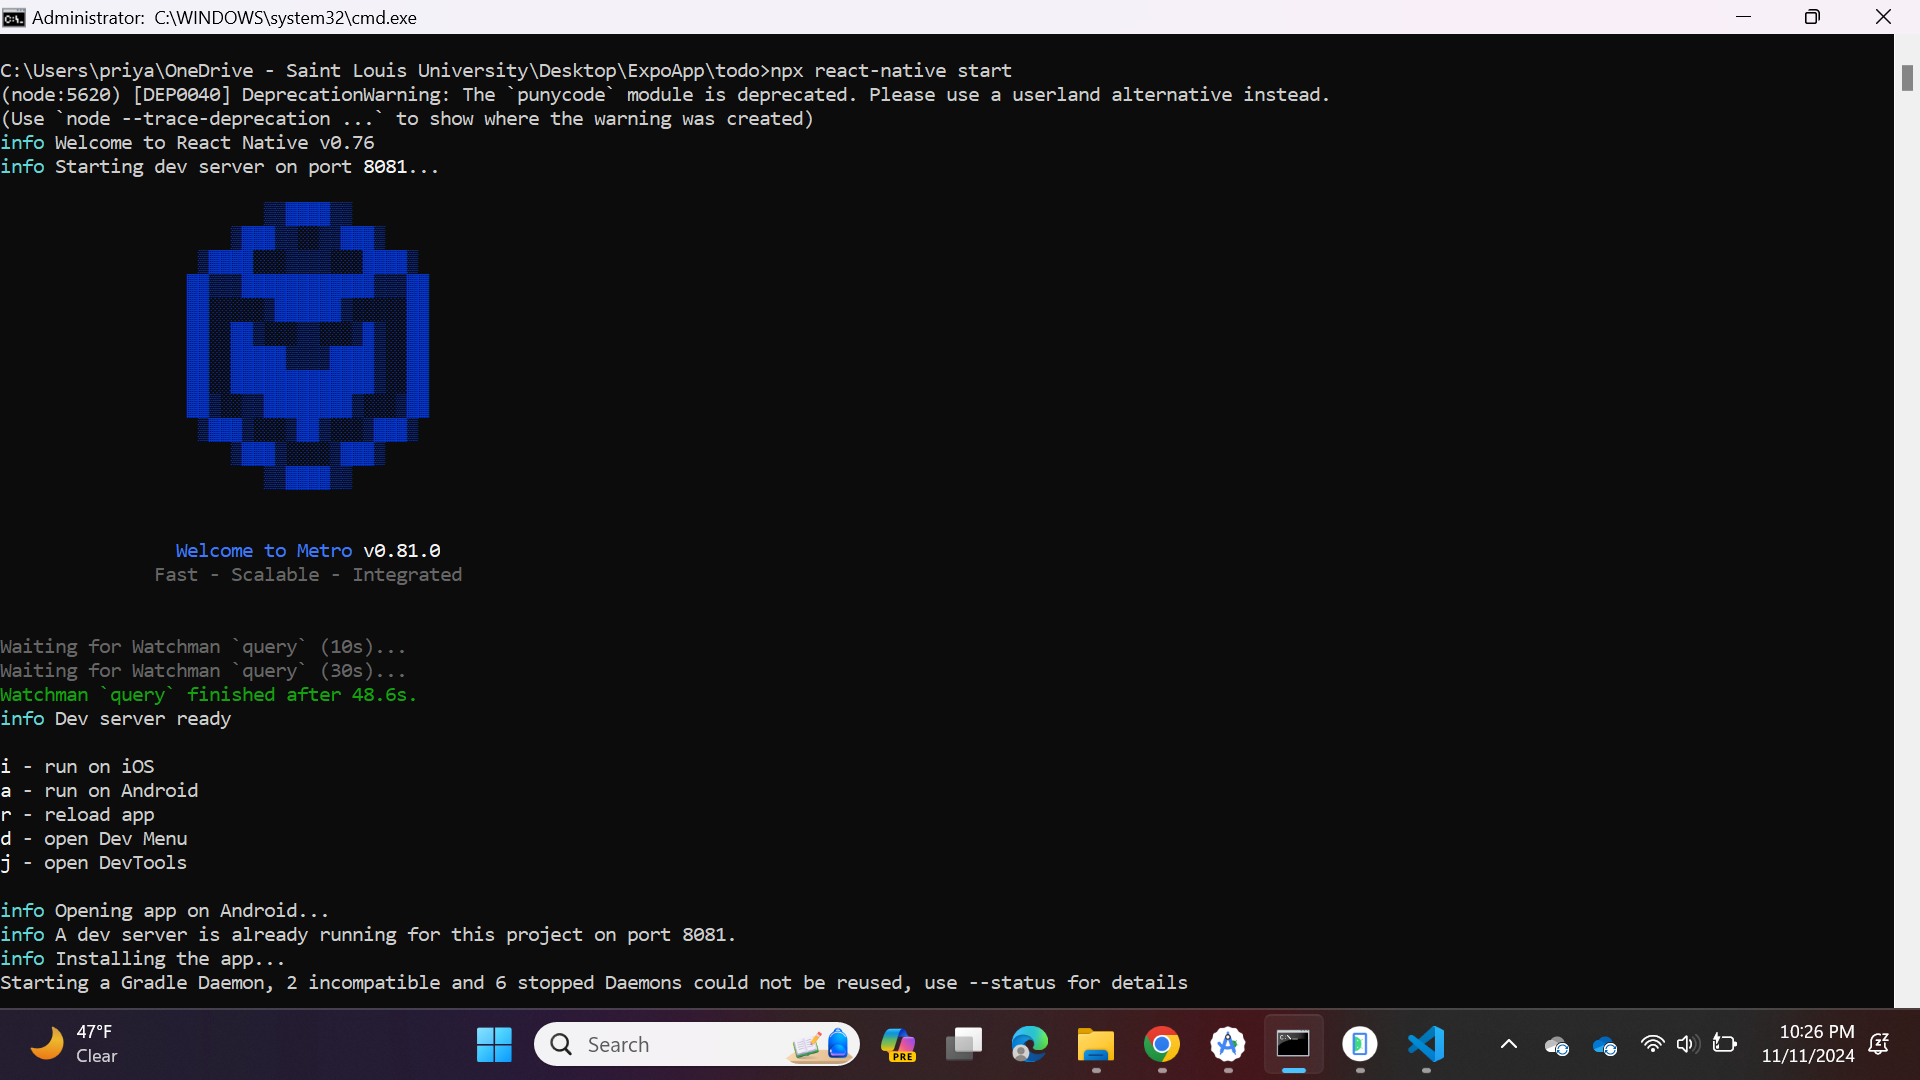
\includegraphics[width=5.57813in,height=3.13391in]{media/image13.png}
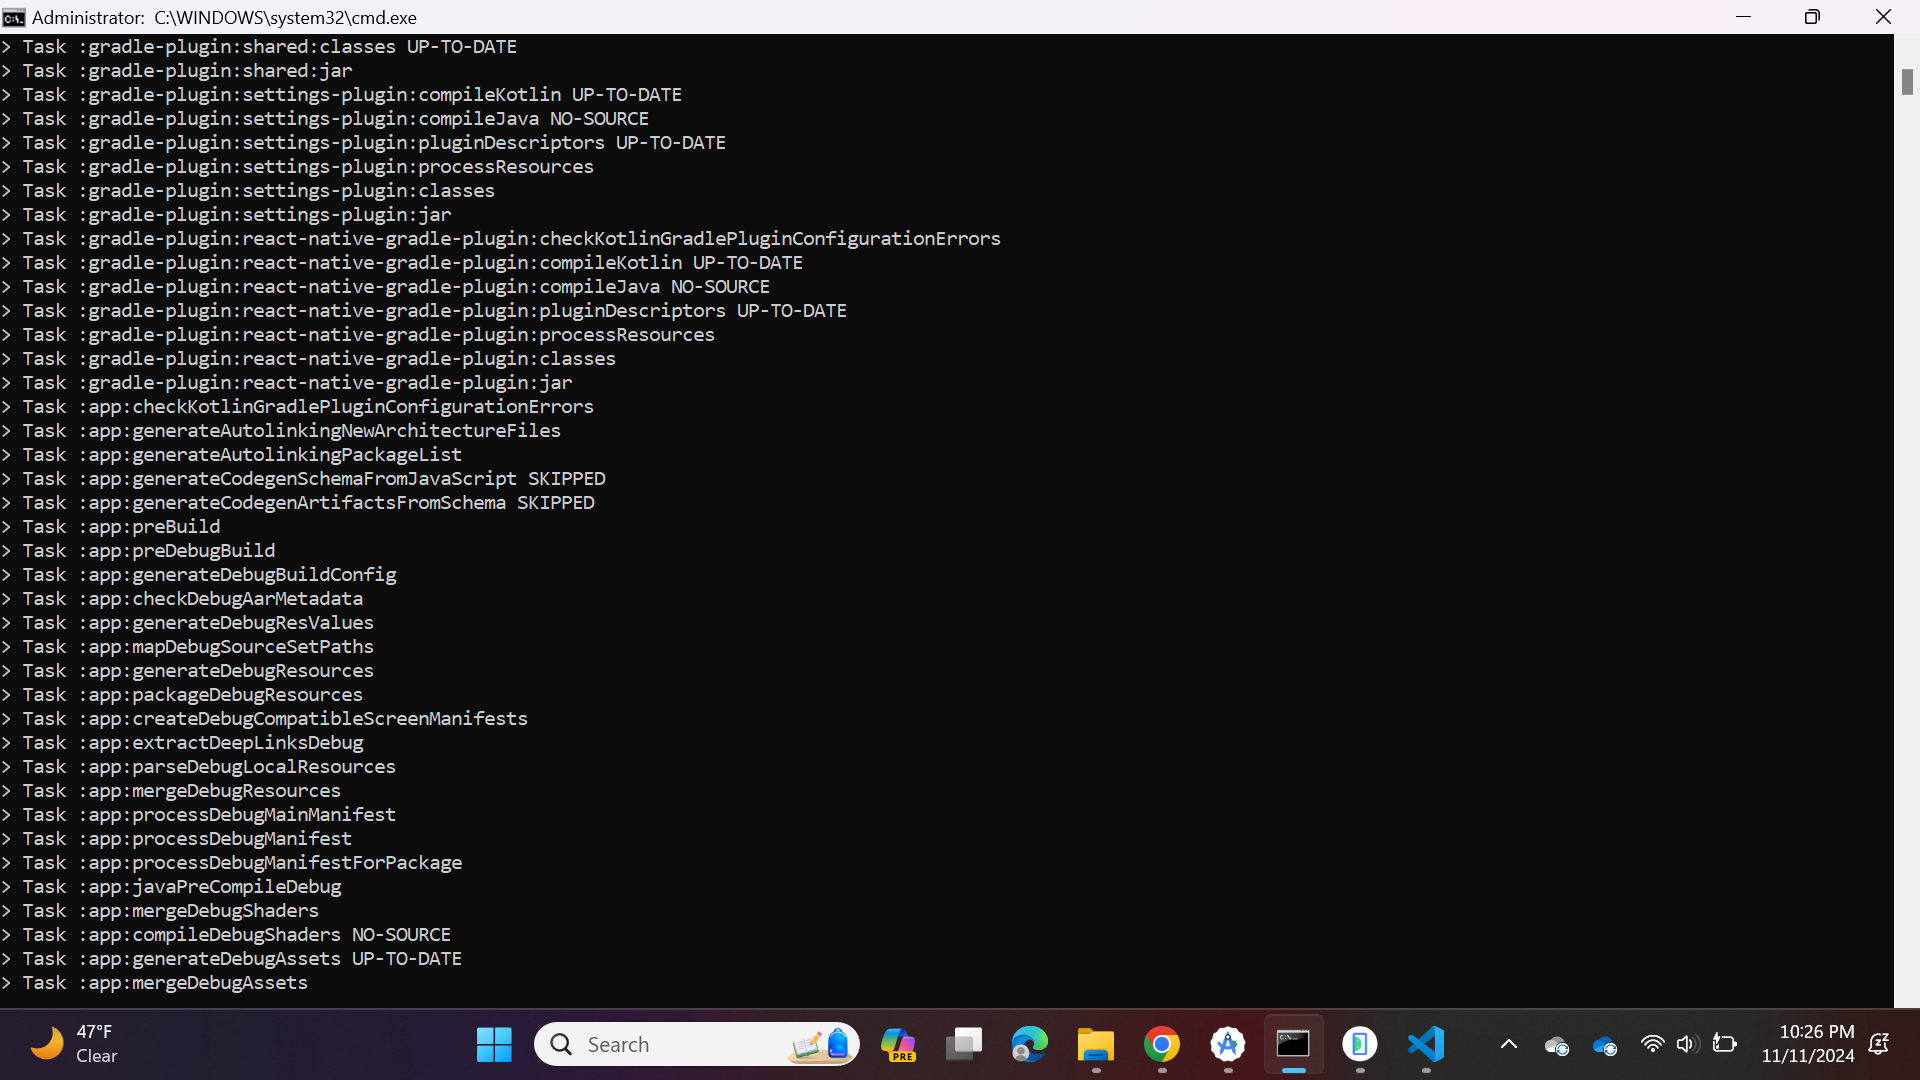
\includegraphics[width=5.57813in,height=3.13391in]{media/image12.png}
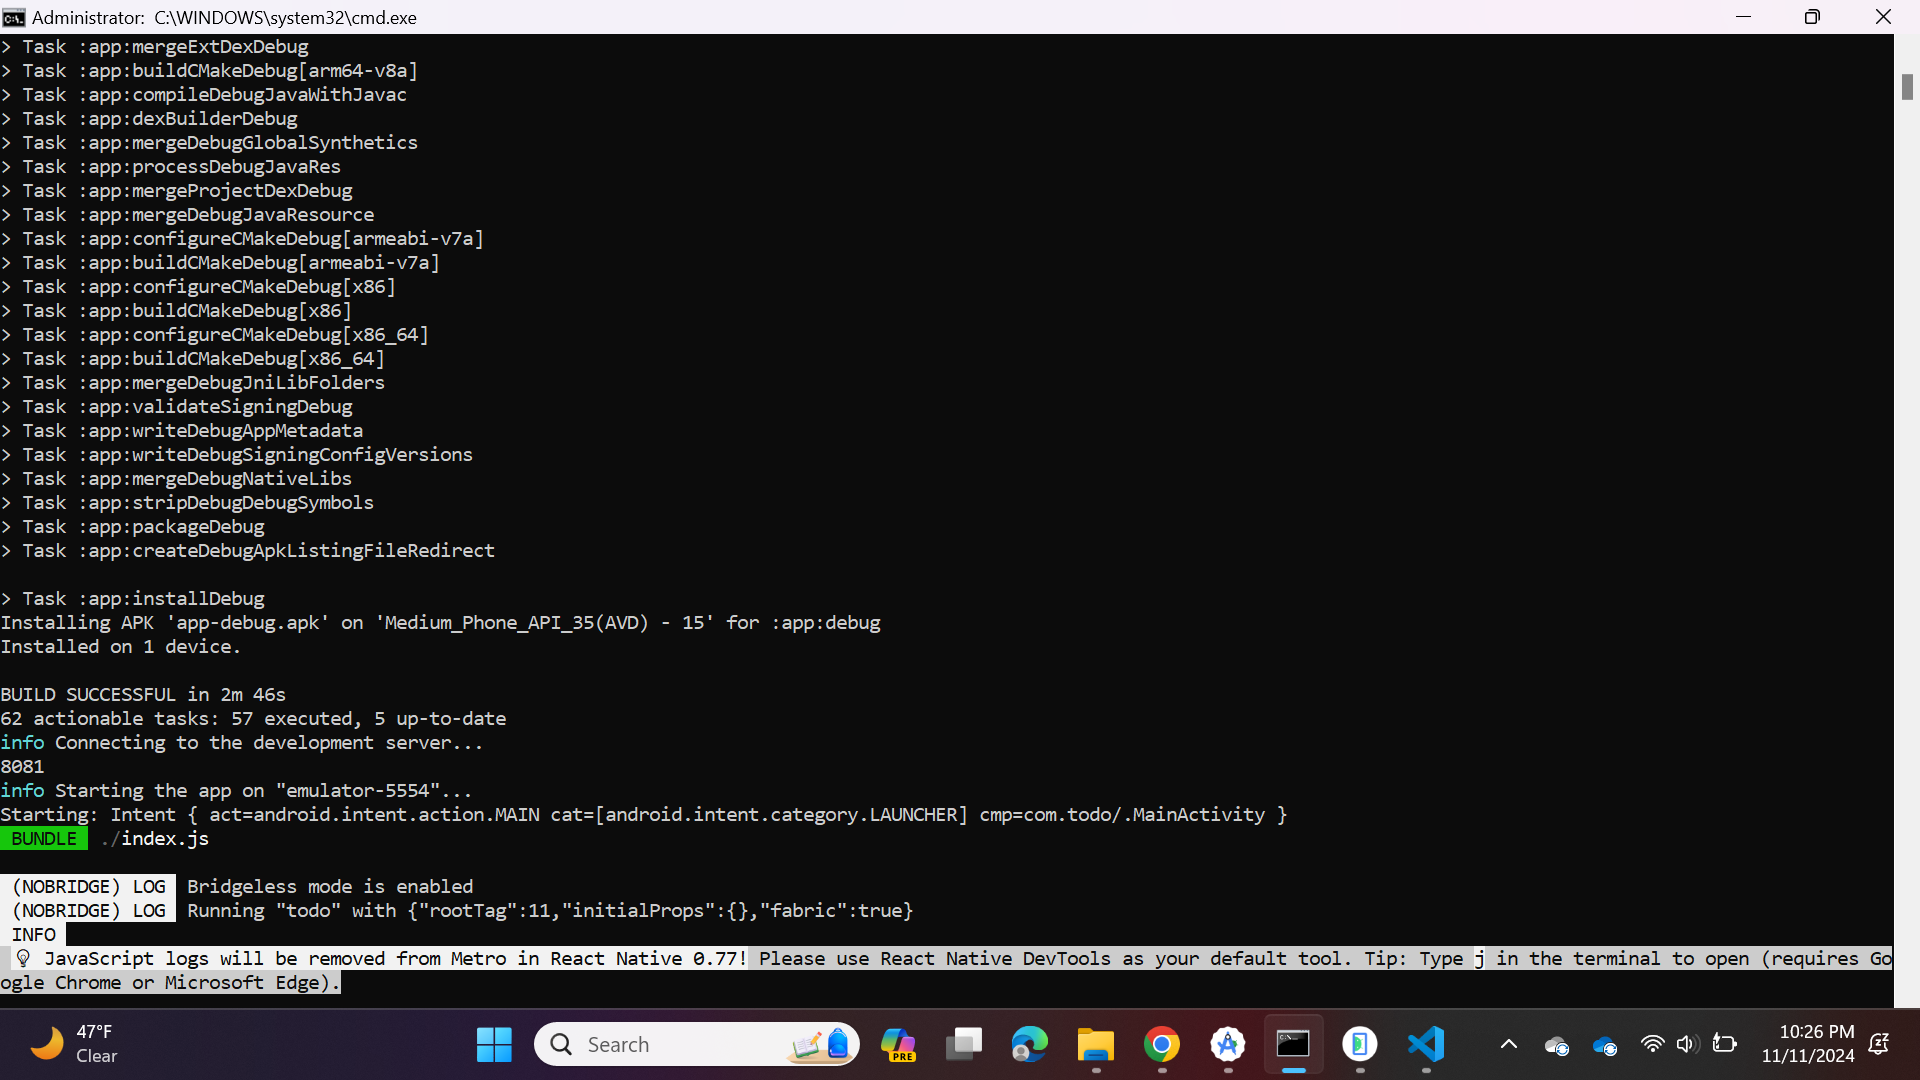
\includegraphics[width=5.57813in,height=3.13391in]{media/image20.png}

\begin{itemize}
    \item This starts the Metro Bundler, which monitors your files and serves JavaScript code.
\end{itemize}


\subsection*{Step 7: Run Your App on an Emulator or Device}

\textbf{For Android:}
\begin{enumerate}
    \item Ensure an emulator is running via Android Studio’s AVD Manager, or connect a physical device with USB debugging enabled.
\end{enumerate}
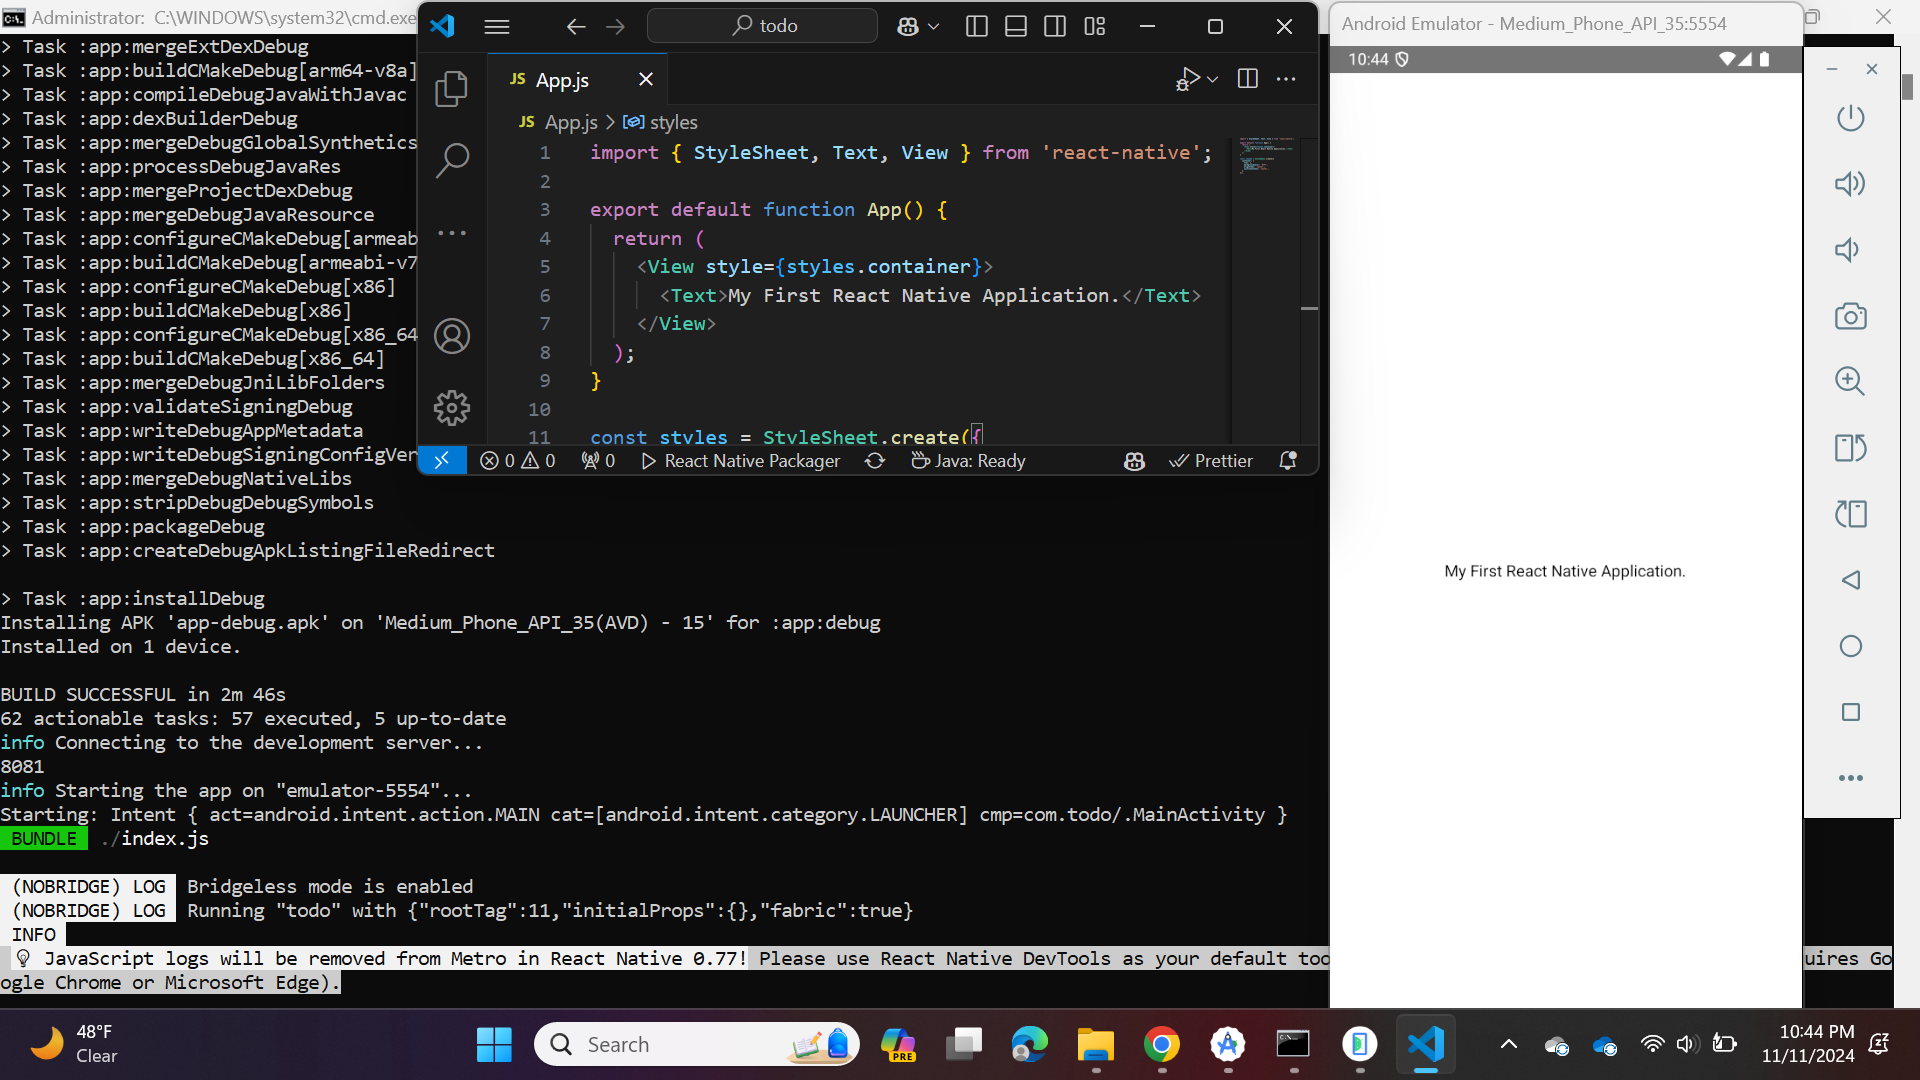
\includegraphics[width=5.57813in,height=3.13391in]{media/image7.png}
    
\begin{enumerate}   
    \item Run:
    \begin{lstlisting}[language=bash]
    npx react-native run-android
    \end{lstlisting}
\end{enumerate}
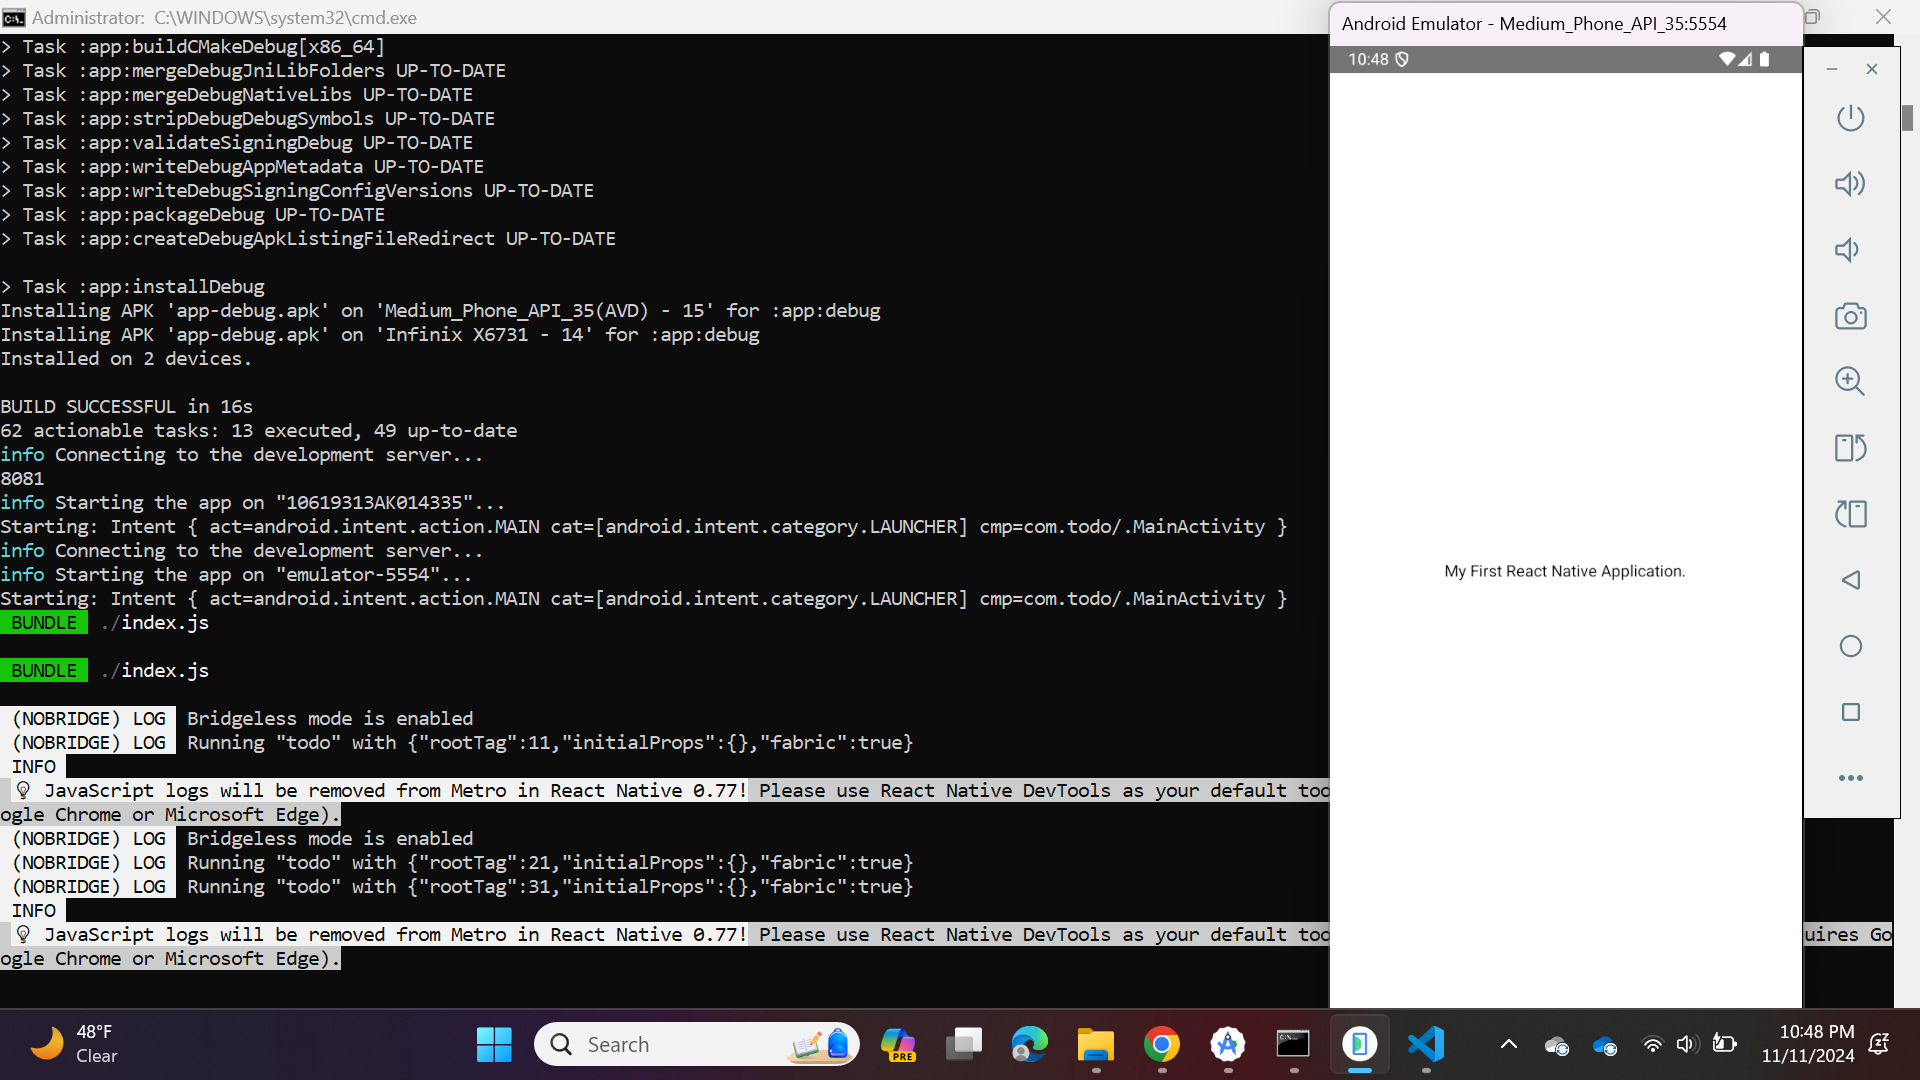
\includegraphics[width=5.57813in,height=3.13391in]{media/image32.png}

\begin{enumerate}
    \item This installs and launches the app on the selected device.
\end{enumerate}
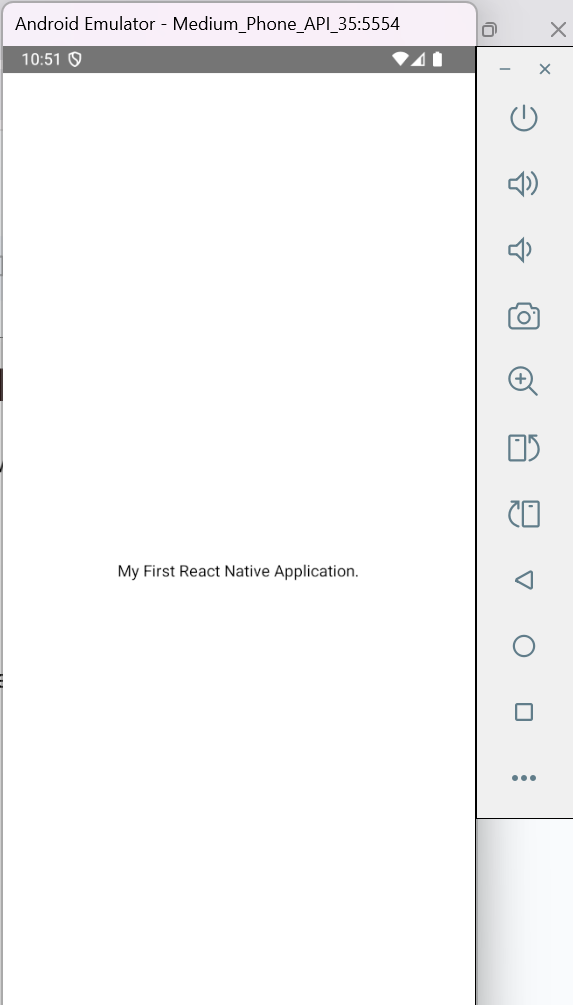
\includegraphics[width=3.14063in,height=5.53233in]{media/image5.png}

\includegraphics[width=2.49141in,height=5.53646in]{media/image6.jpg}


\subsection*{Step 8: Run Your App on a Mobile Device Using Expo}

\begin{enumerate}
    \item Install Expo CLI and create a new project:
    \begin{lstlisting}[language=bash]
    npm install -g expo-cli
    npx expo init YourProjectName
    cd YourProjectName
    npx expo start
    \end{lstlisting}
\end{enumerate}
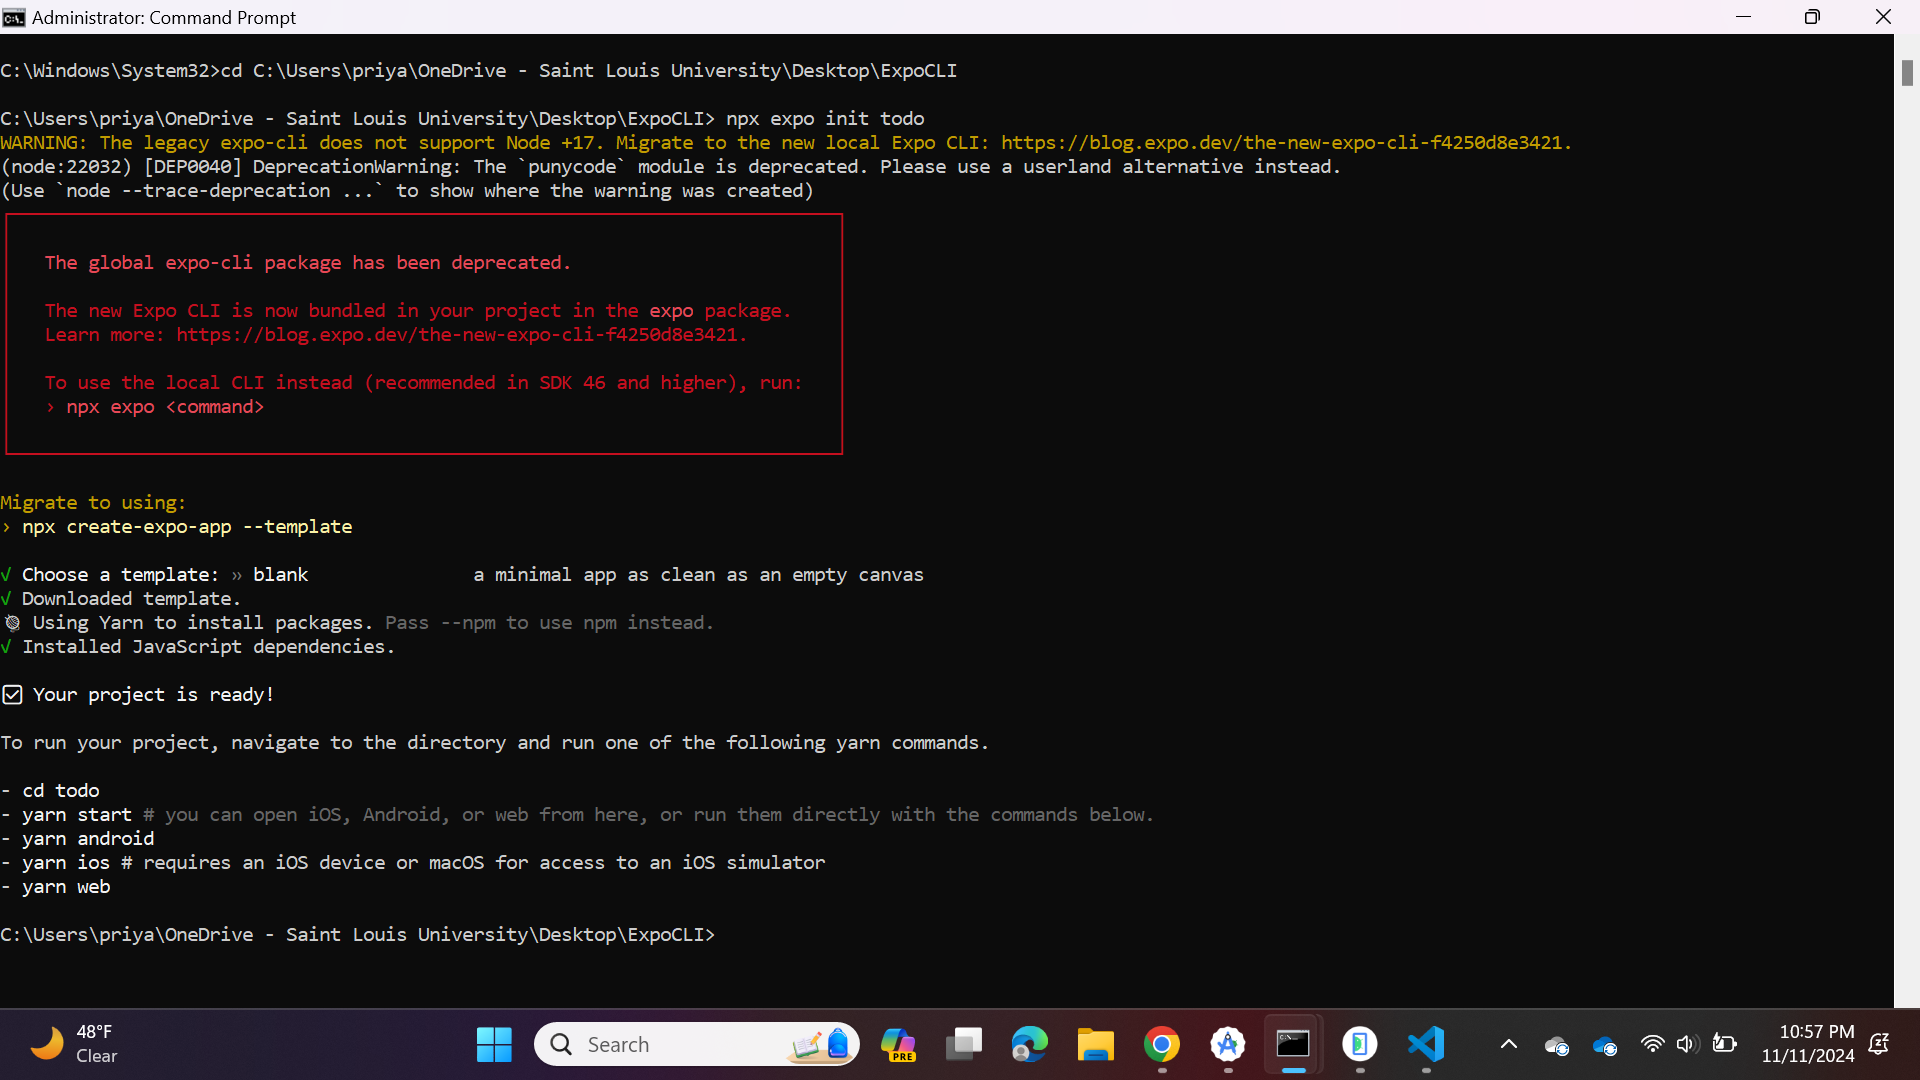
\includegraphics[width=5.57813in,height=3.13391in]{media/image36.png}
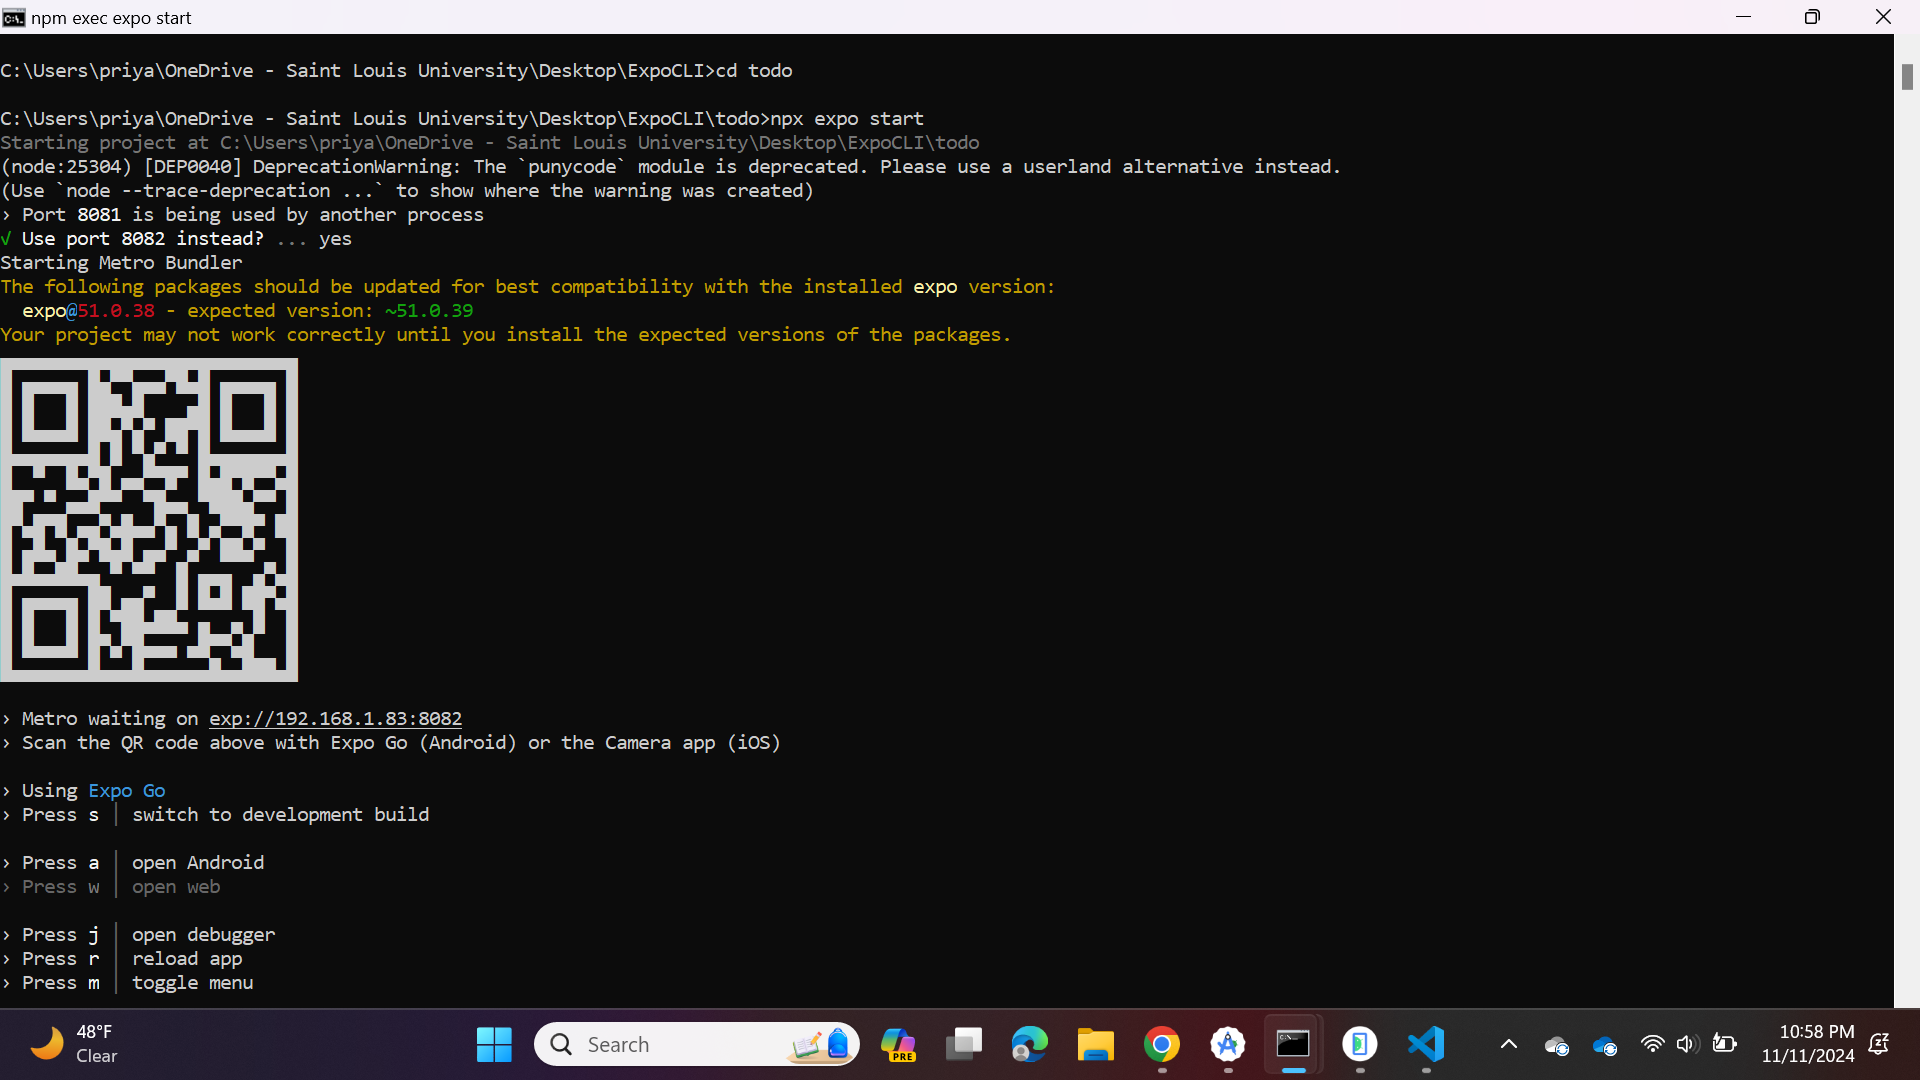
\includegraphics[width=5.57813in,height=3.13391in]{media/image28.png}
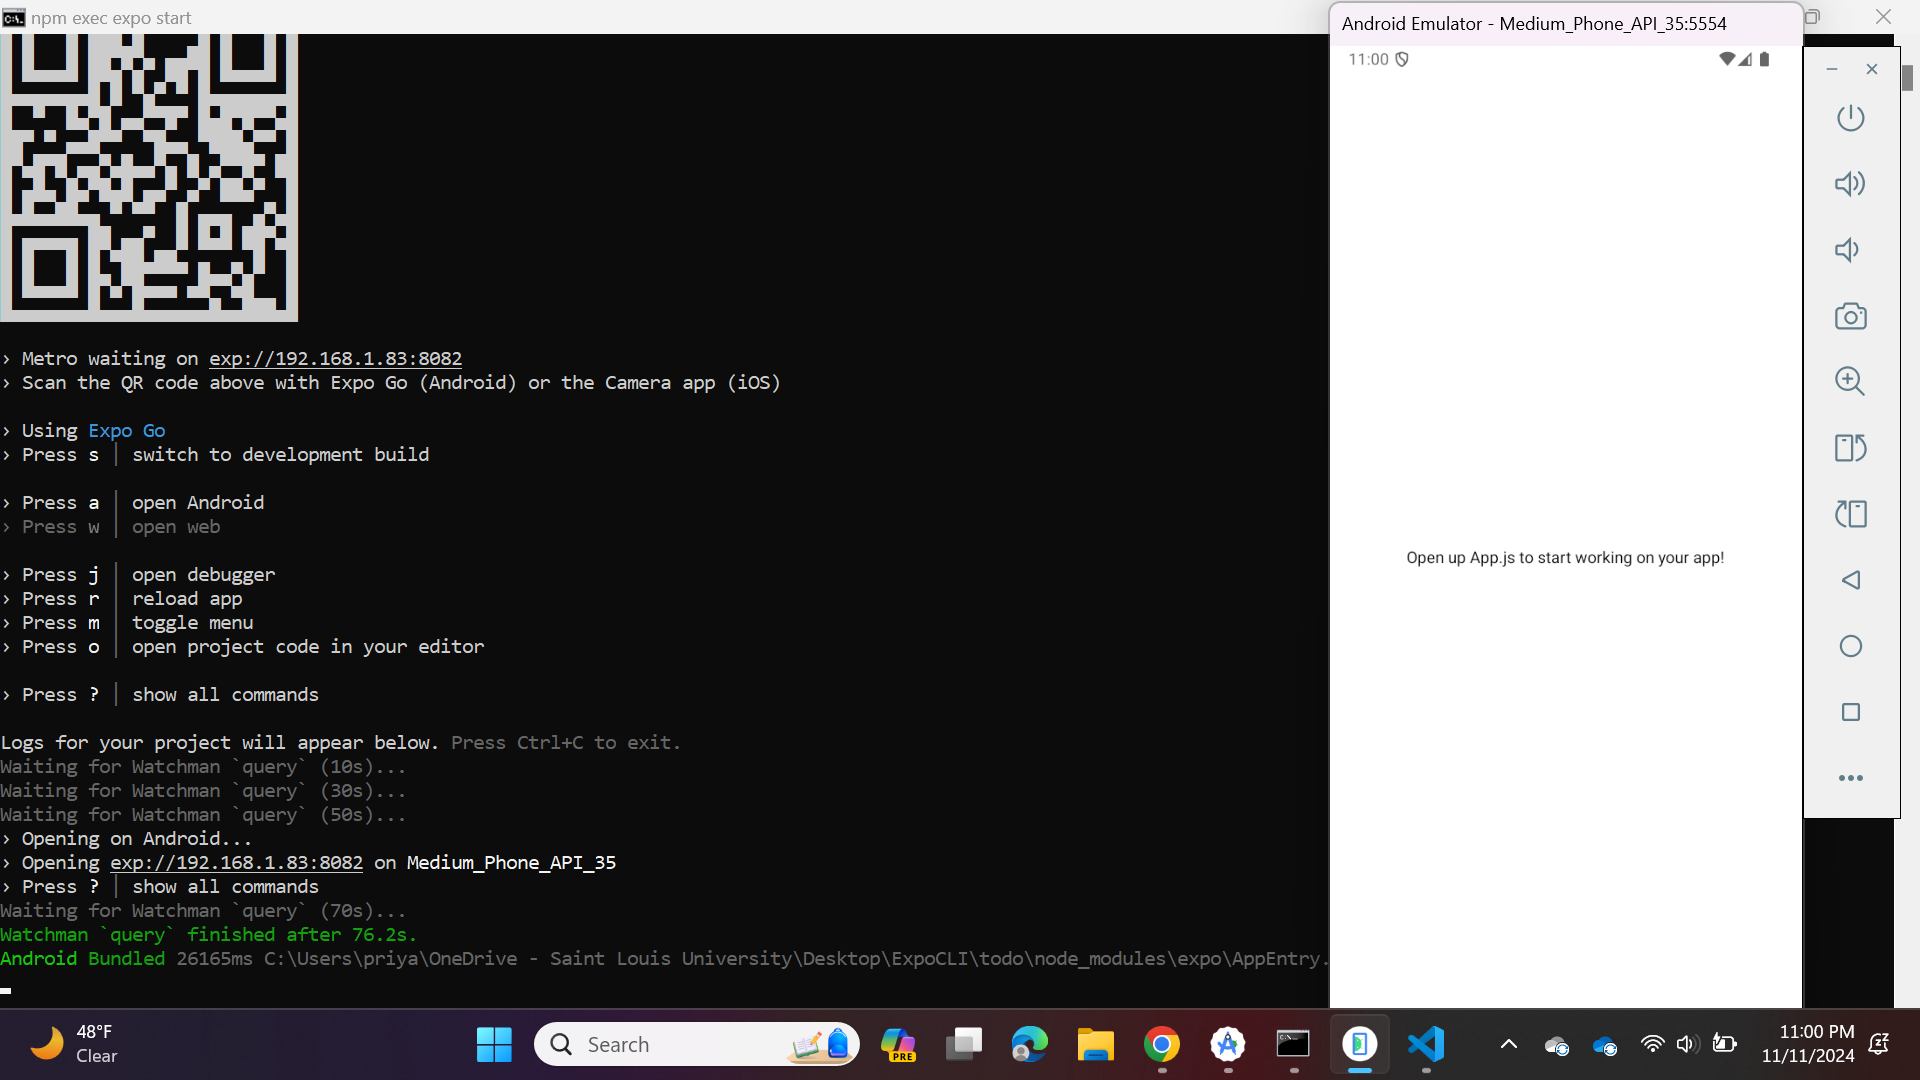
\includegraphics[width=5.57813in,height=3.13391in]{media/image35.png}


\begin{enumerate}
    \item Connect your mobile device to the same Wi-Fi network.
\end{enumerate}
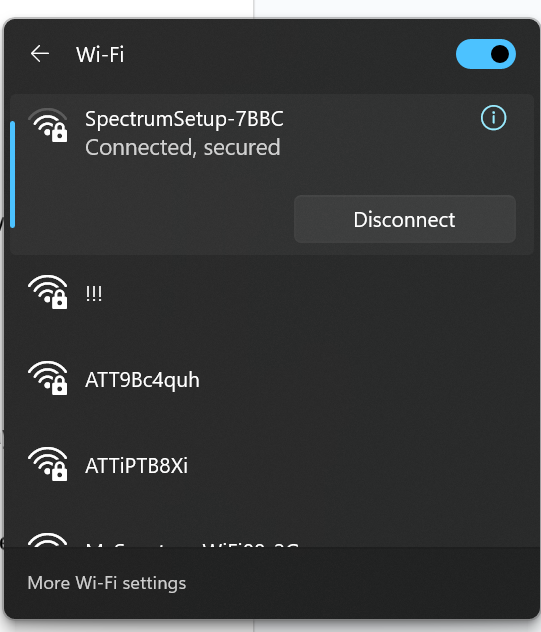
\includegraphics[width=3.38839in,height=3.95313in]{media/image17.png}
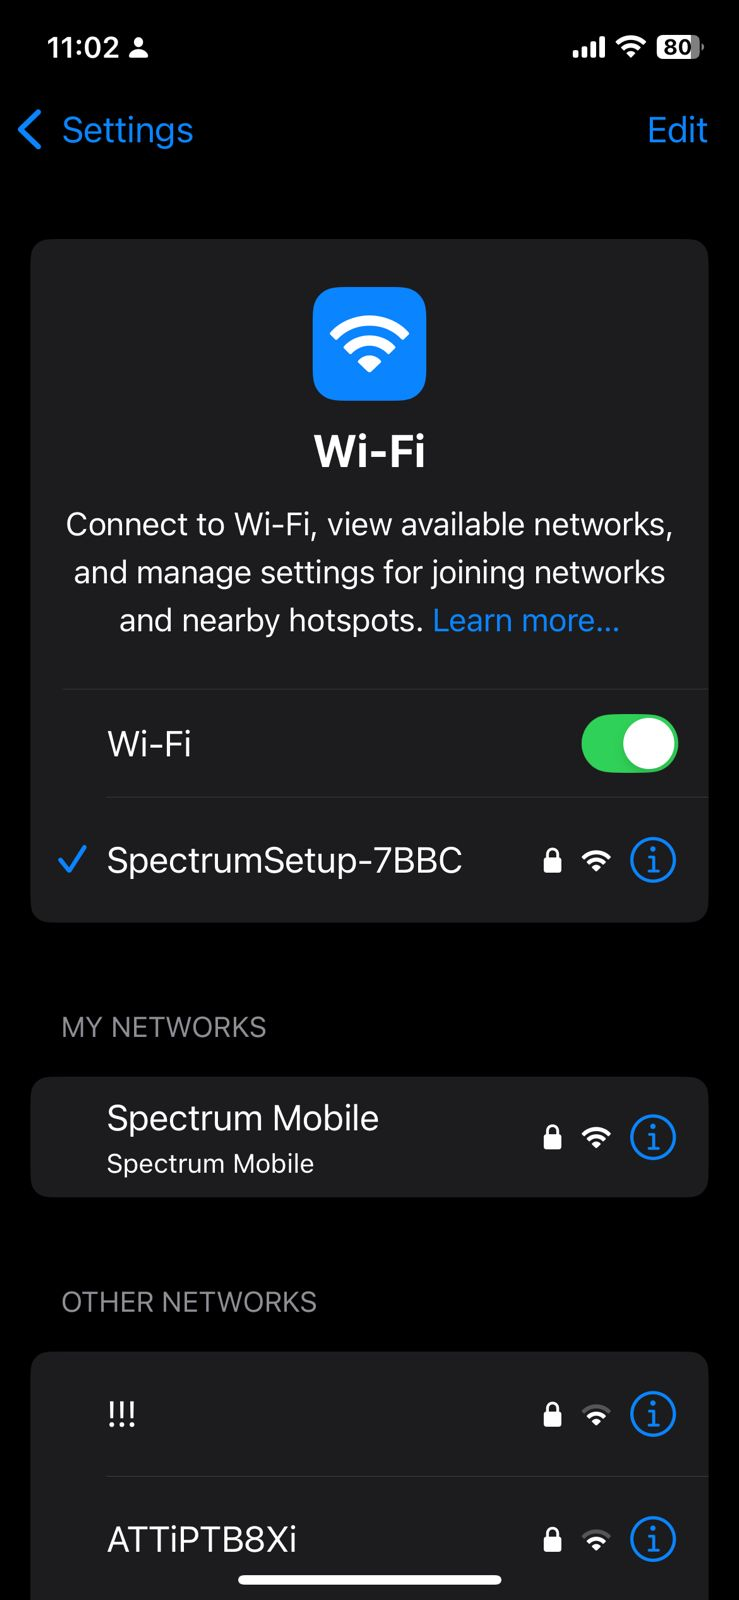
\includegraphics[width=2.70173in,height=5.85938in]{media/image19.jpg}

\begin{enumerate}
    \item Install the Expo Go app from the App Store or Google Play Store.
\end{enumerate}
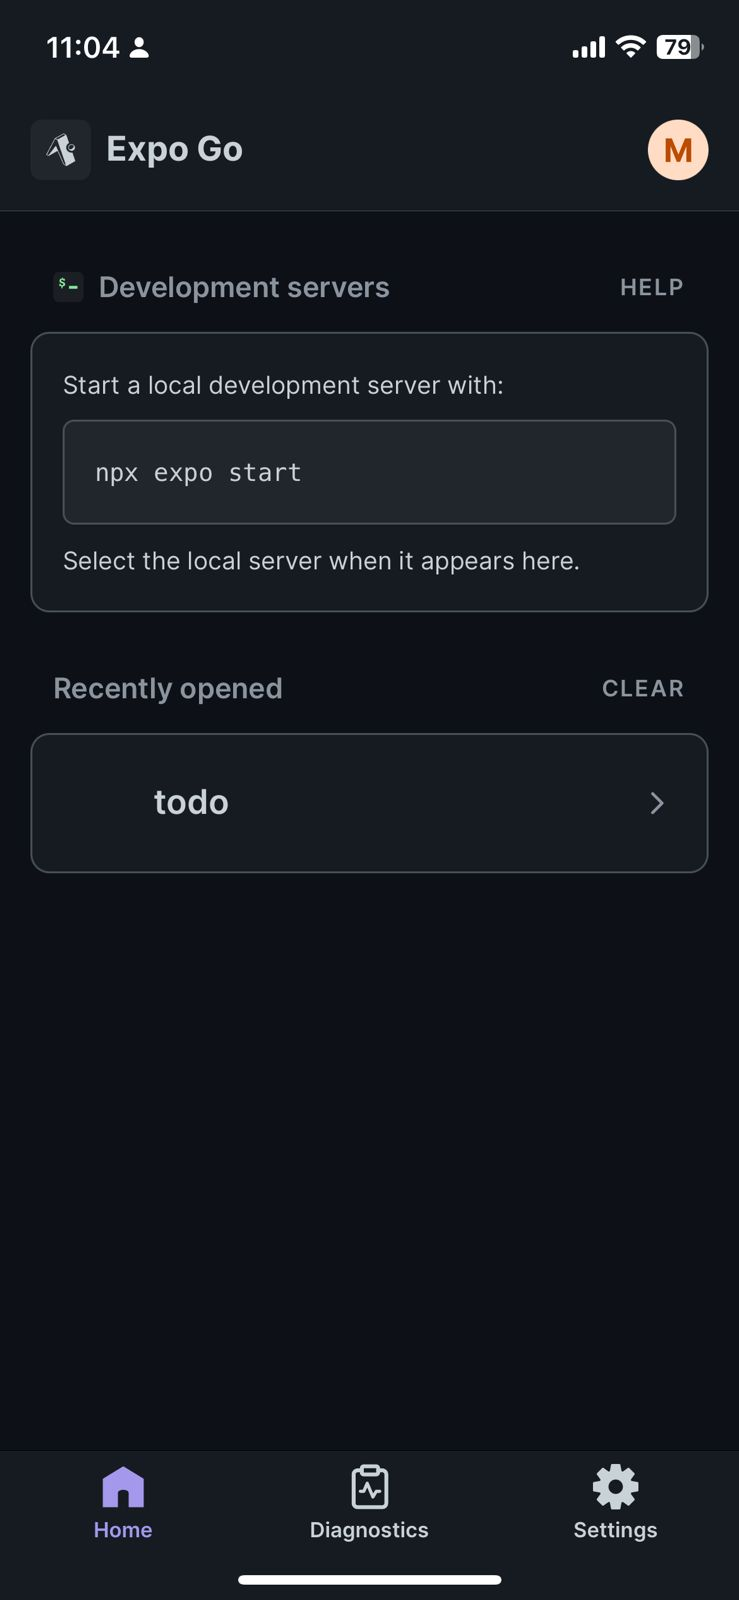
\includegraphics[width=2.49141in,height=5.53646in]{media/image4.jpg} 

\begin{enumerate}
    \item Scan the QR code provided in the Expo developer tools to launch the app.
\end{enumerate}
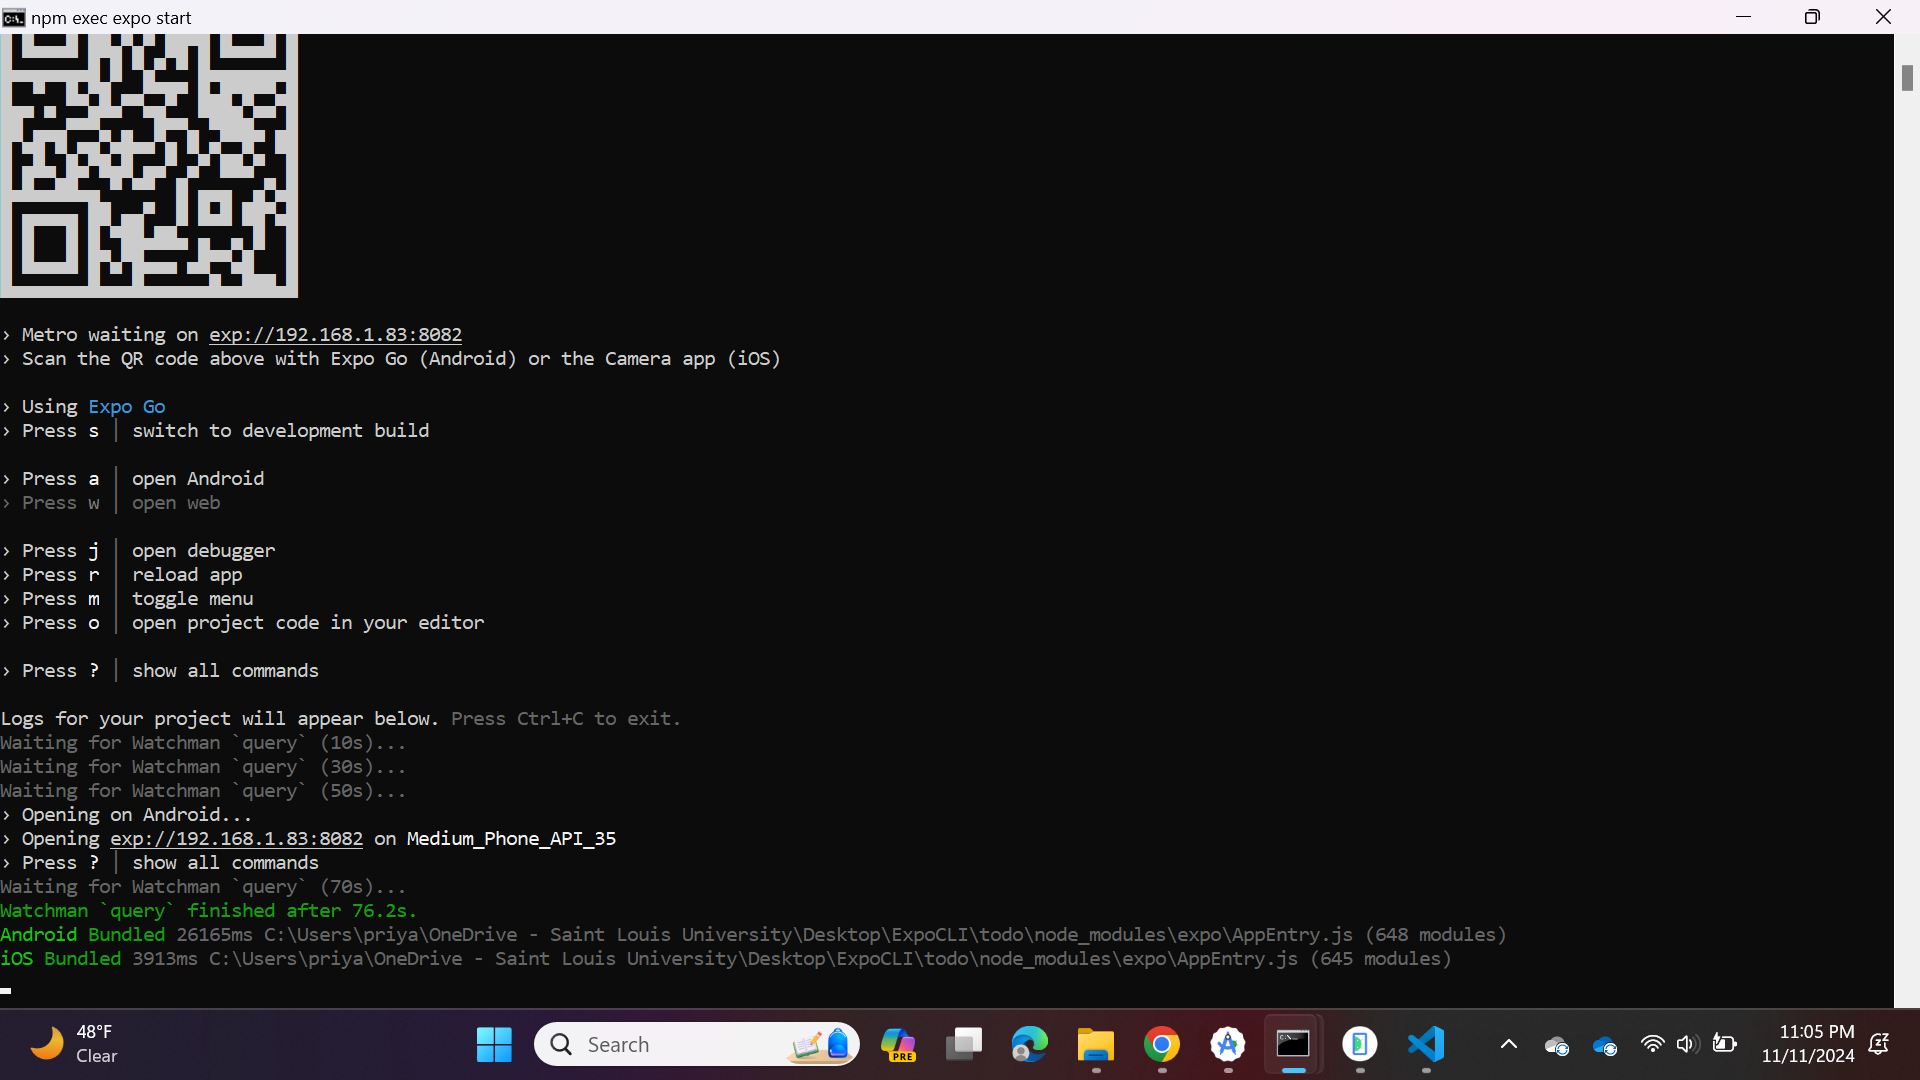
\includegraphics[width=5.57813in,height=3.13391in]{media/image25.png}
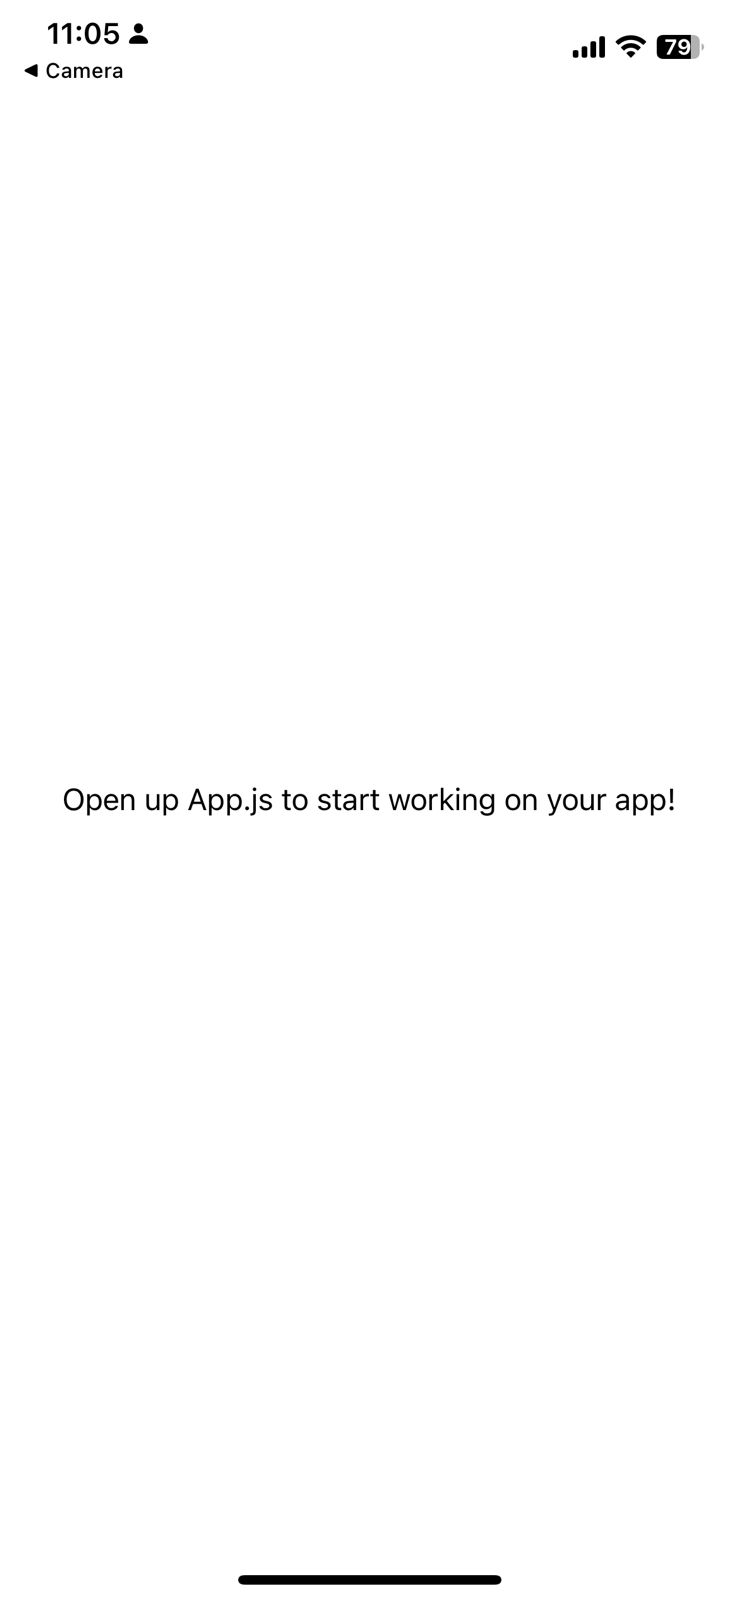
\includegraphics[width=2.49141in,height=5.53646in]{media/image3.jpg}
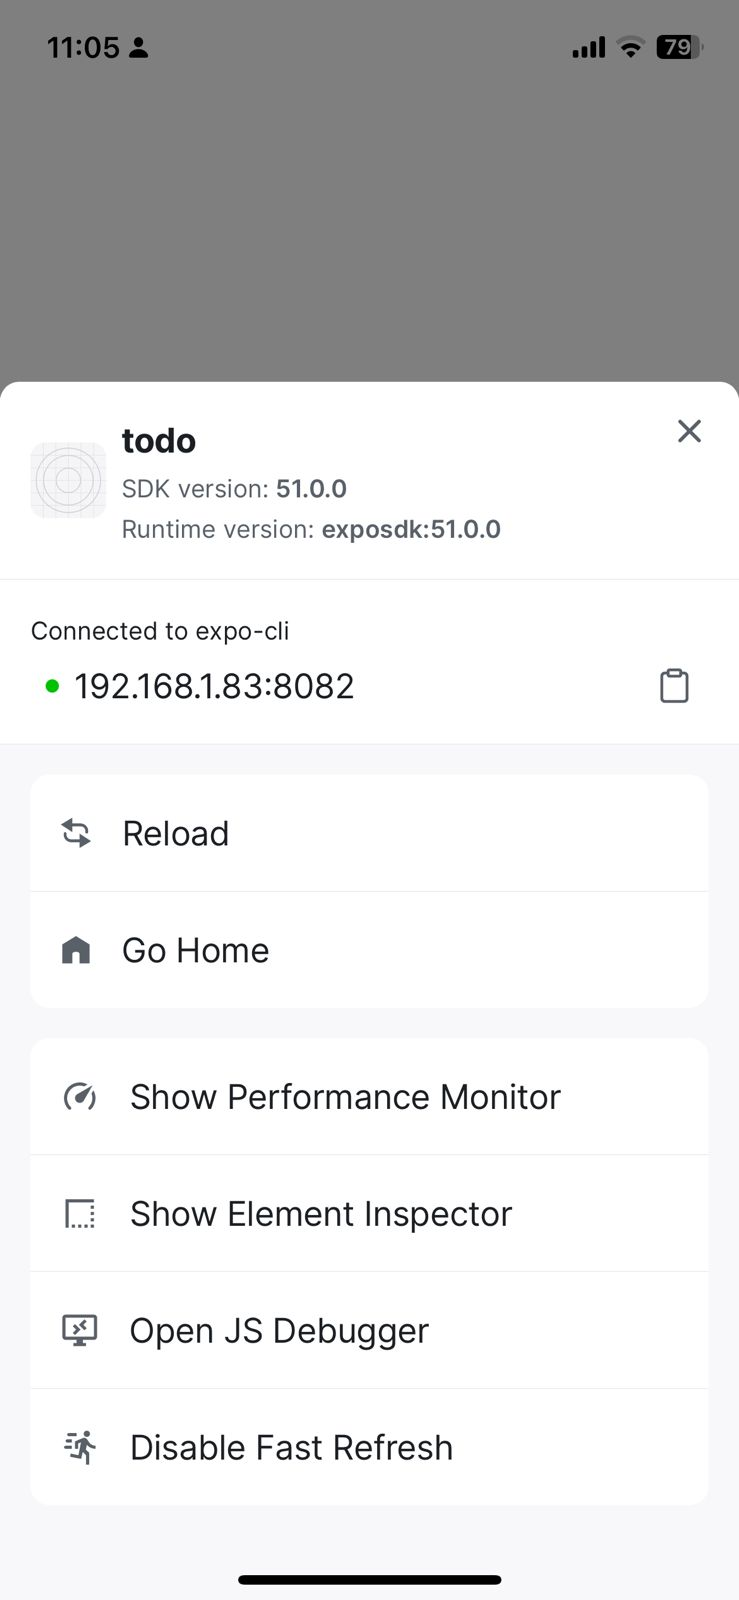
\includegraphics[width=2.49141in,height=5.53646in]{media/image21.jpg}


\section*{What to Submit for Task 1 (Total 40 Points)}

\subsection*{1. Screenshots of Your App (5 Points)}
\begin{itemize}
    \item Attach screenshots of your app running on an emulator and on a physical Android or iOS device.
\end{itemize}
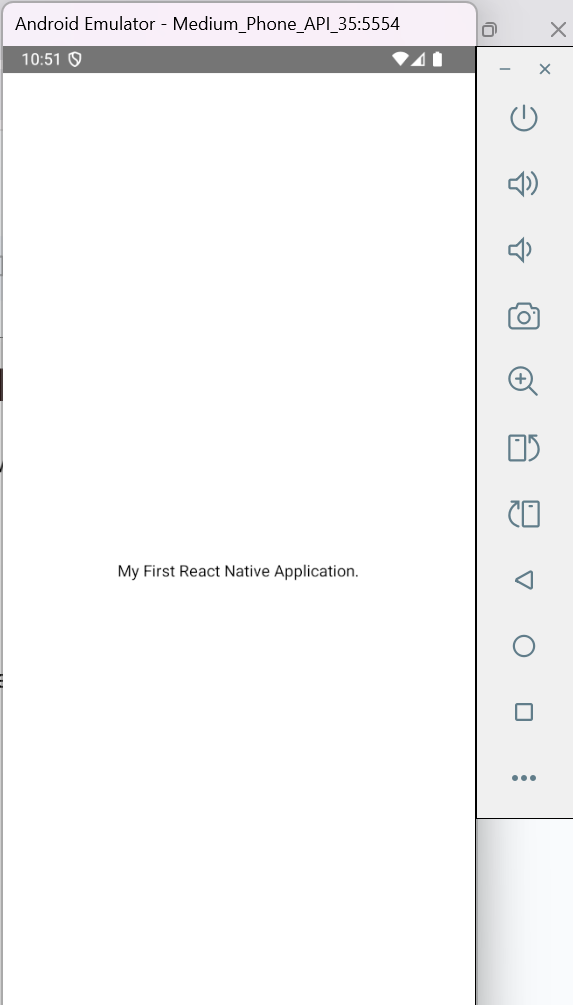
\includegraphics[width=3.14063in,height=5.53233in]{media/image5.png}

\includegraphics[width=2.49141in,height=5.53646in]{media/image6.jpg}

\begin{itemize}
    \item Describe any differences you observed between running the app on an emulator versus a physical device.

    When running the app on an emulator, it felt slower compared to a physical device, which was much faster. The graphics on the emulator sometimes lagged or looked slightly different, while the physical device displayed the UI more accurately. Also, using the emulator meant relying on a mouse and keyboard for gestures, but the physical device allowed for real touch interactions, making it more intuitive.
    
\end{itemize}

\subsection*{2. Setting Up an Emulator (10 Points)}
\begin{itemize}
    \item Explain the steps you followed to set up an emulator in Android Studio or Xcode.

    \begin{itemize}
    
    \item I opened Android Studio and went to the AVD Manager.
    \item I created a virtual device by selecting a phone model (e.g., Pixel 4).
    \item Then, I downloaded the Android version I needed and set the emulator's settings like RAM and storage.
    \item After that, I clicked the play button to launch the emulator.
    
    \end{itemize}

    \item Discuss any challenges you faced during the setup and how you overcame them.

    \begin{itemize}
    
    \item The emulator was really slow.
    \item I also had trouble with a specific Android version.

    \end{itemize}


\end{itemize}

\subsection*{3. Running the App on a Physical Device Using Expo (10 Points)}
\begin{itemize}
    \item Describe how you connected your physical device to run the app using Expo.

     \begin{itemize}
    
    \item I downloaded the Expo Go app on my phone.
    \item I made sure my phone and computer were on the same Wi-Fi.
    \item I started the app on my computer using expo start and scanned the QR code with my phone's Expo Go app.

    \end{itemize}
    
    \item Include any troubleshooting steps if you encounter issues.

    \begin{itemize}
    
    \item Once, my phone wasn’t on the same Wi-Fi as my computer, so I connected them to the same network, and it worked fine.

    \item Sometimes, the QR code wouldn’t work, so I copied the link from the terminal and opened it manually in the Expo Go app.

    \end{itemize}
\end{itemize}

\subsection*{4. Comparison of Emulator vs. Physical Device (10 Points)}
\begin{itemize}
    \item Compare and contrast using an emulator versus a physical device for React Native development.

     \begin{itemize}
    
    \item Emulator:

     \begin{itemize}
    
    \item Slower and sometimes lags.
    \item Simulates touch with a mouse, which isn’t natural.
    \item Easy to set up and test on different virtual devices.

    \end{itemize}

    \item Physical Device:

     \begin{itemize}
    
    \item Faster and shows real-world performance.
    \item Lets you test real touch gestures.
    \item Takes more effort to set up but gives accurate results.

    \end{itemize}

    \end{itemize}
    
    \item Discuss the advantages and disadvantages of each option.

    \begin{itemize}
    
    \item Advantages:

     \begin{itemize}
    
    \item Easy to set up and use.
    \item Runs faster and shows exactly how users will experience the app.
    \item Can test on lots of "fake" devices with different screen sizes.

    \end{itemize}

    \item Disadvantages:

     \begin{itemize}
    
    \item Slower and sometimes laggy.
    \item Takes more effort to set up.
    \item Harder to test on different types of devices unless you have several phones.

    \end{itemize}

    \end{itemize}
    
\end{itemize}

\subsection*{5. Troubleshooting a Common Error (5 Points)}
\begin{itemize}
    \item Identify a common error you encountered when starting your React Native app. Note that it is very unlikely that everyone will get the same error here.

    I faced dependencies error where my jdk wasn't compatible with the running react-native version. I had to run npx react-native doctor to find the loose dependencies.

    \item Explain the cause of the error and the steps you took to resolve it.

    This caused due to incompatible jdk version. To solve this I download jdk-17 restarted the computer and ran the run-android command again to start the app.
    
\end{itemize}

\section*{Task 2: Building a Simple To-Do List App}

\subsection*{Step 1: Set Up the Project}

\begin{itemize}
    \item Create a new project:
    \begin{lstlisting}[language=bash]
    npx react-native init SimpleTodoApp
    cd SimpleTodoApp
    \end{lstlisting}
\end{itemize}
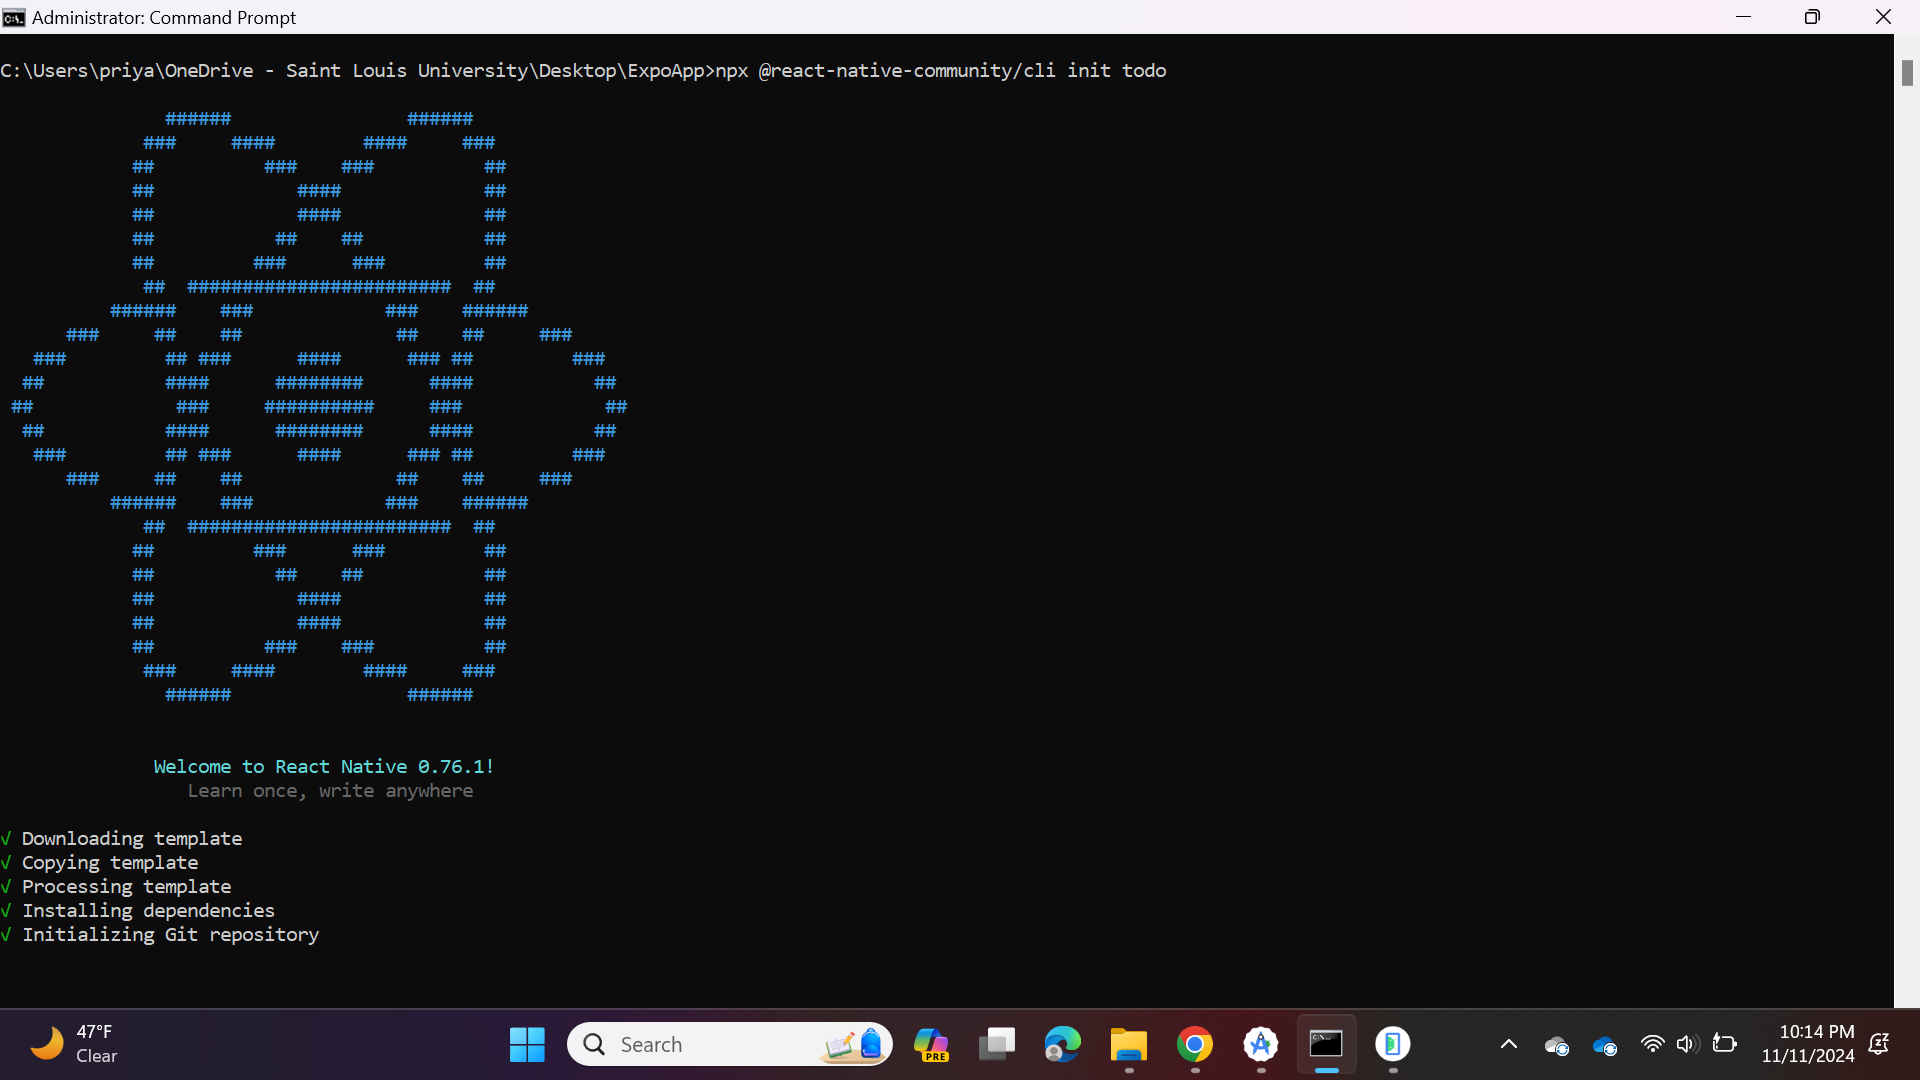
\includegraphics[width=5.57813in,height=3.13391in]{media/image10.png}
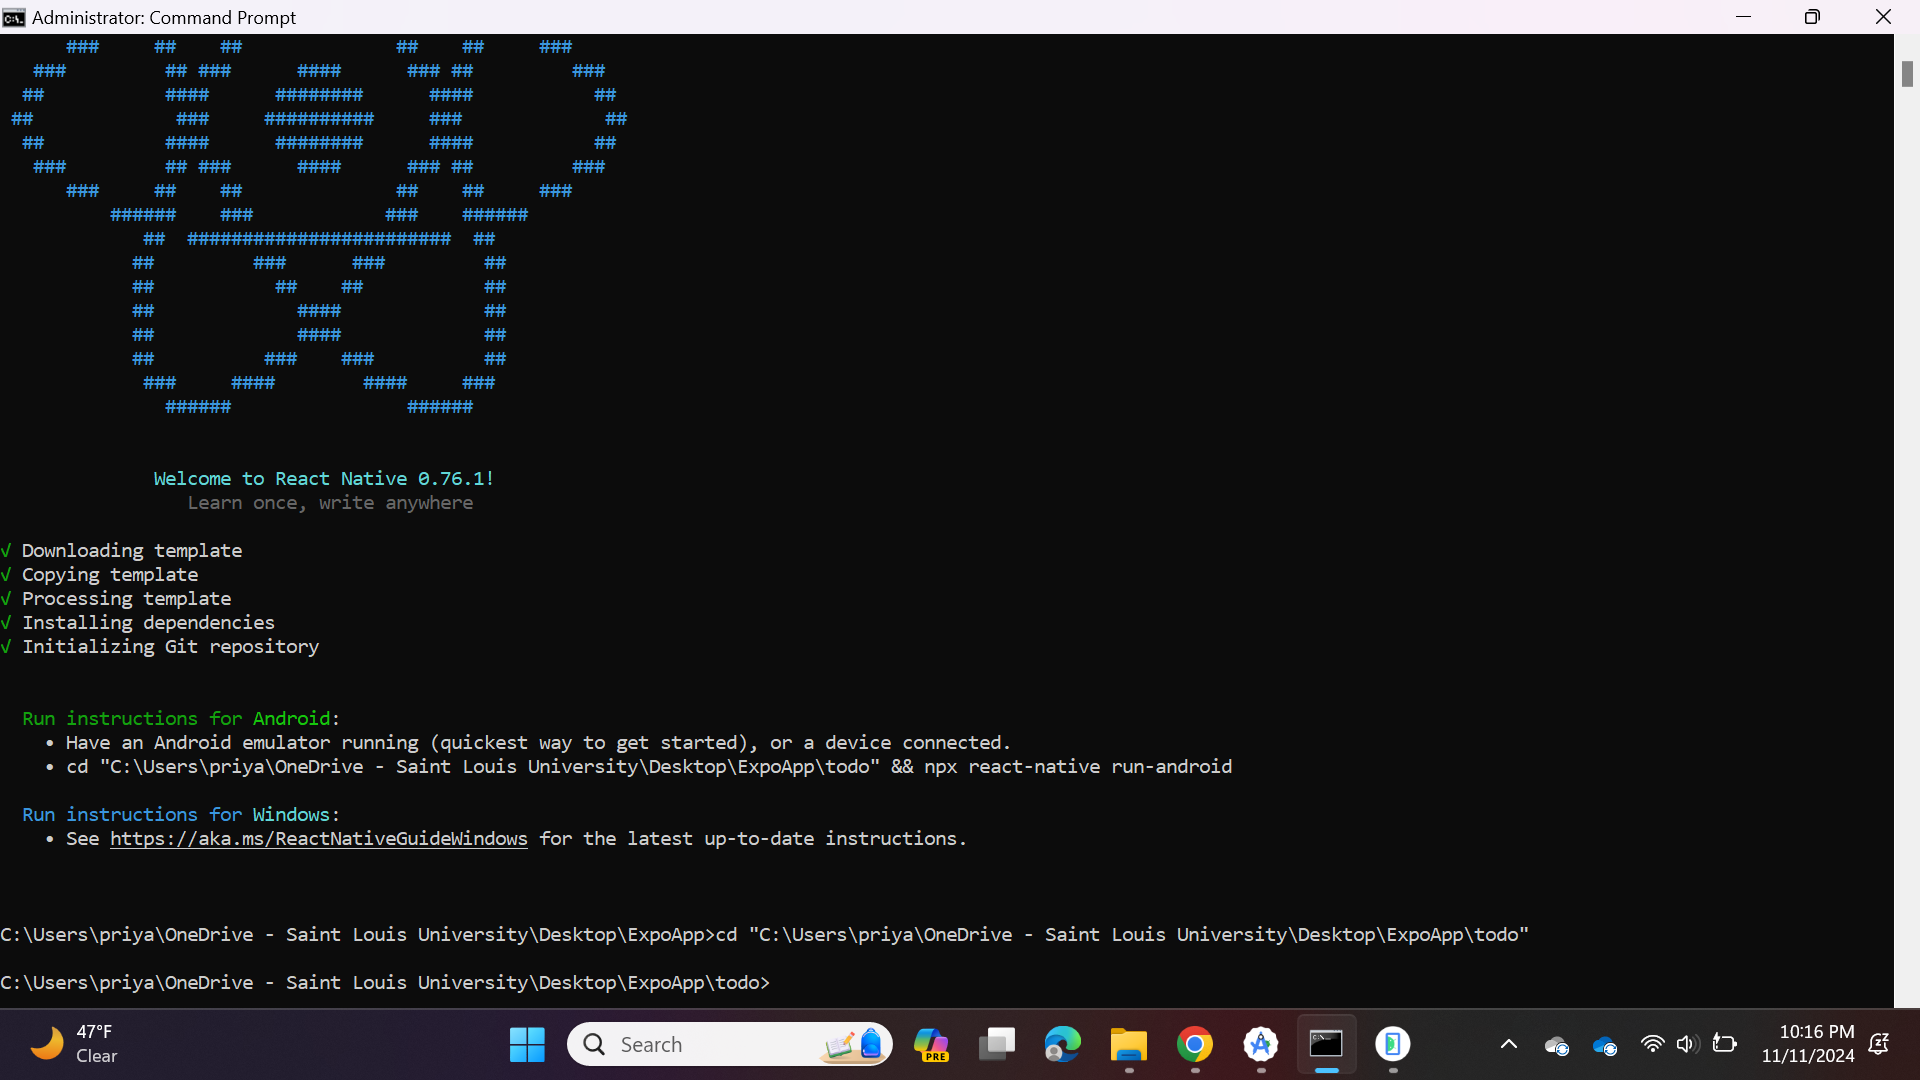
\includegraphics[width=5.57813in,height=3.13391in]{media/image18.png}

\begin{itemize}
    \item Open the project in VS Code:
    \begin{lstlisting}[language=bash]
    code .
    \end{lstlisting}
\end{itemize}
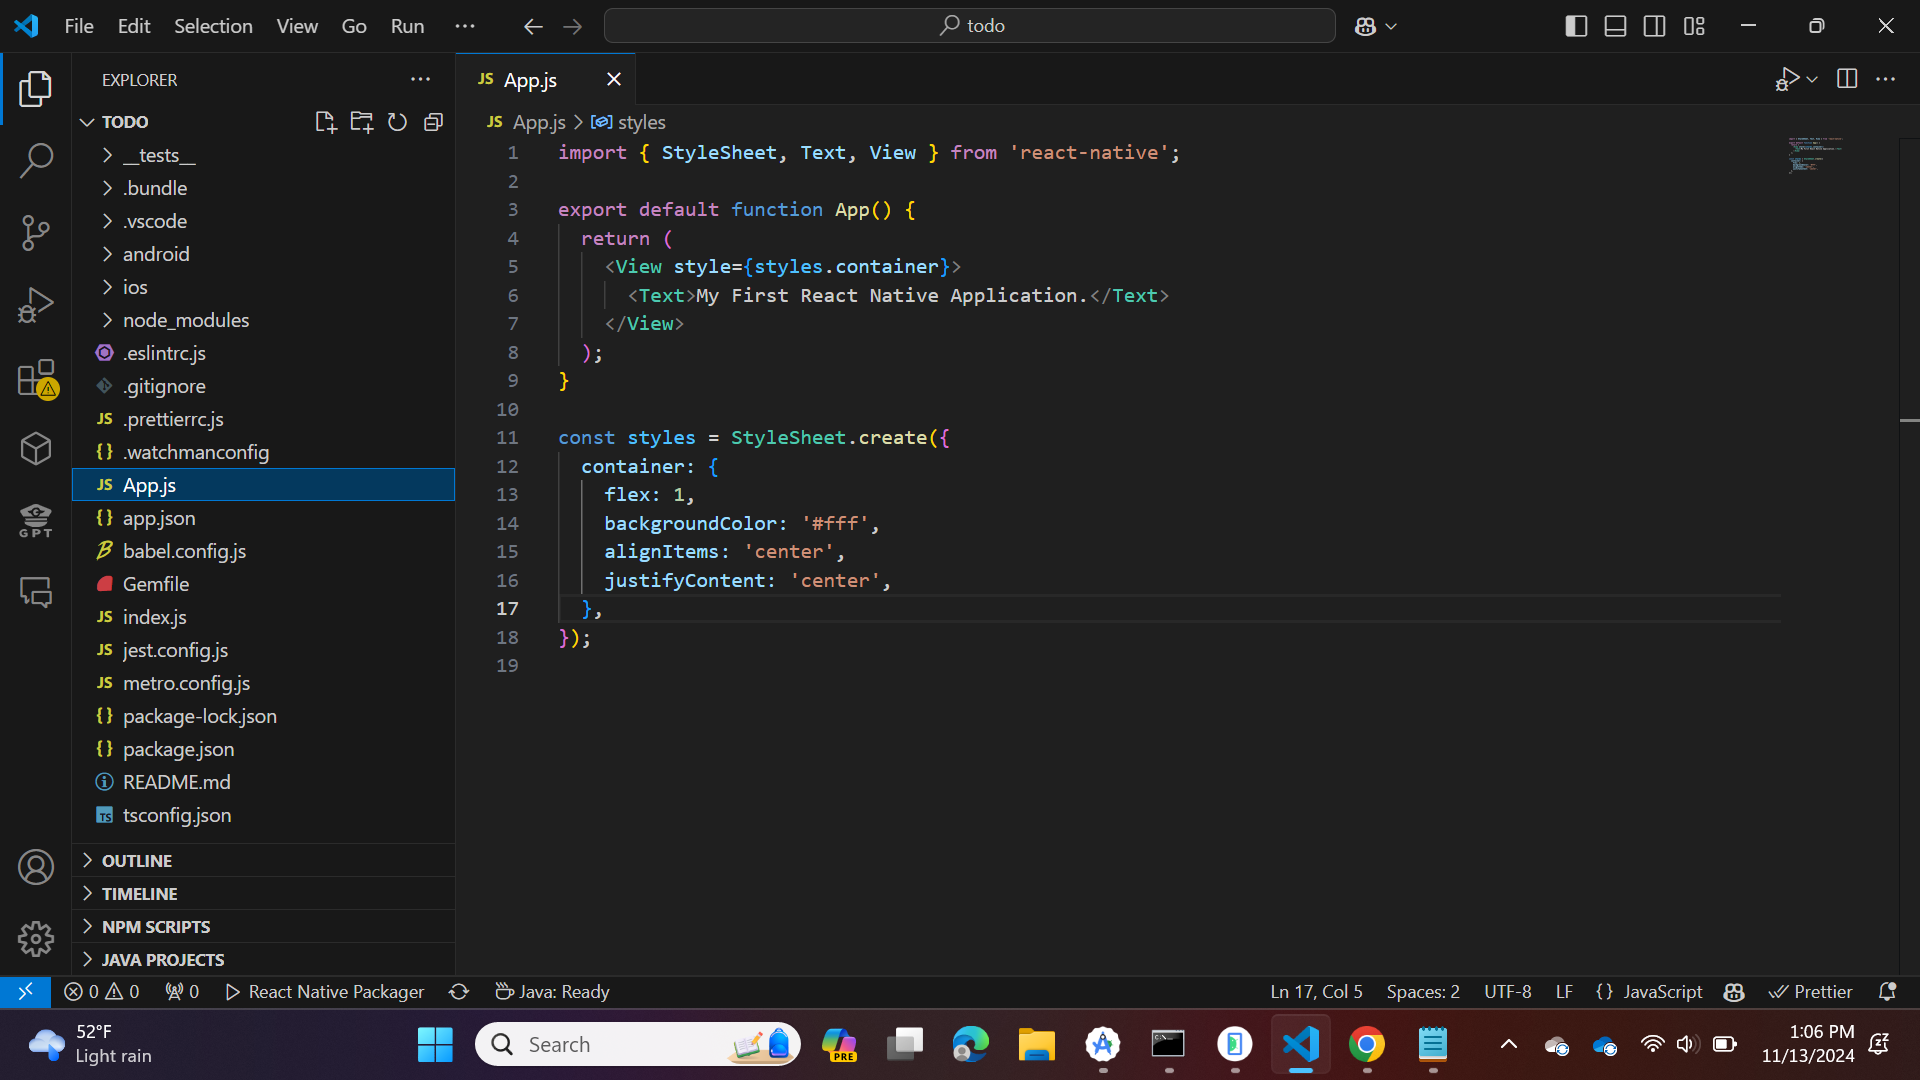
\includegraphics[width=5.57813in,height=3.13391in]{media/image14.png}

    
\subsection*{Step 2: Create the Basic To-Do List Structure}

\begin{description}
Replace the content of \texttt{App.js} with a basic structure for the To-Do list.
\end{description}
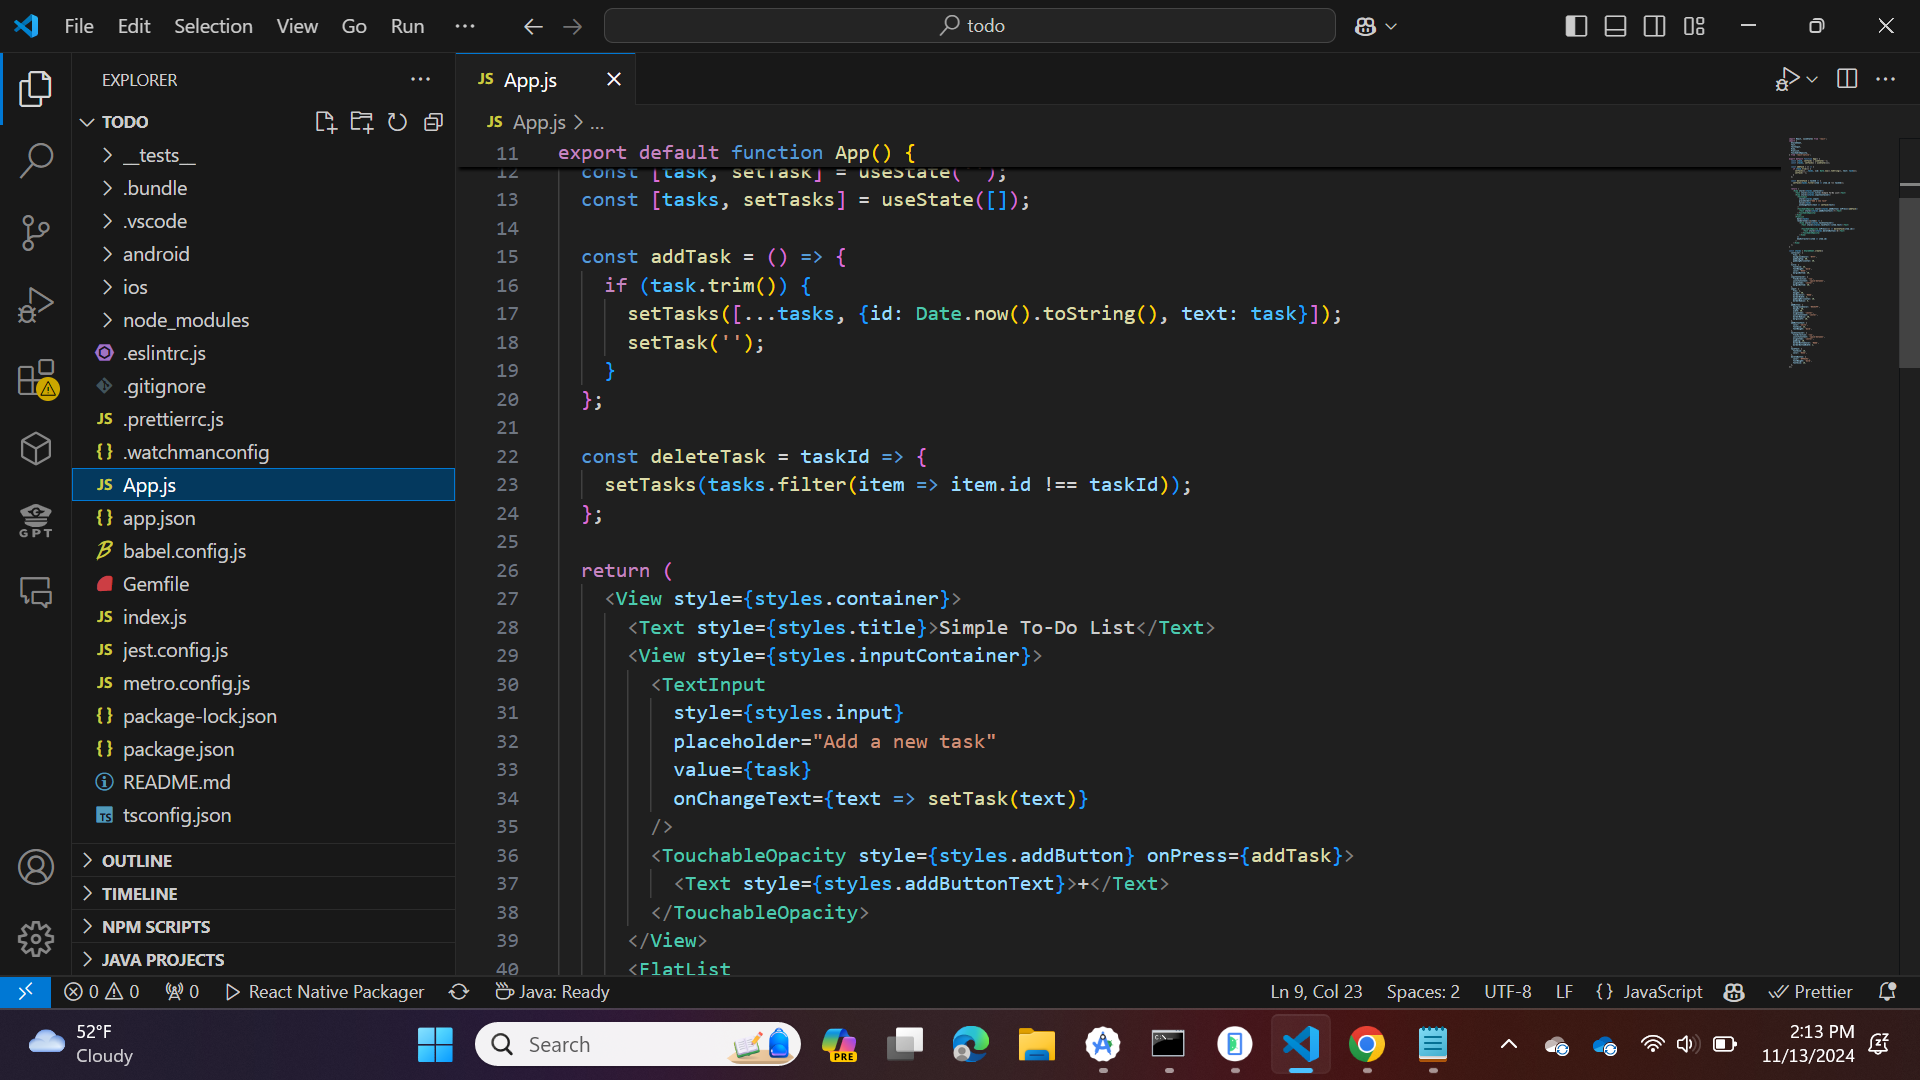
\includegraphics[width=5.57813in,height=3.13391in]{media/image30.png}

\subsection*{Step 3: Add Styles for the To-Do List}

\begin{description}
Add personalized styles to the bottom of \texttt{App.js} to improve the UI.
\end{description}
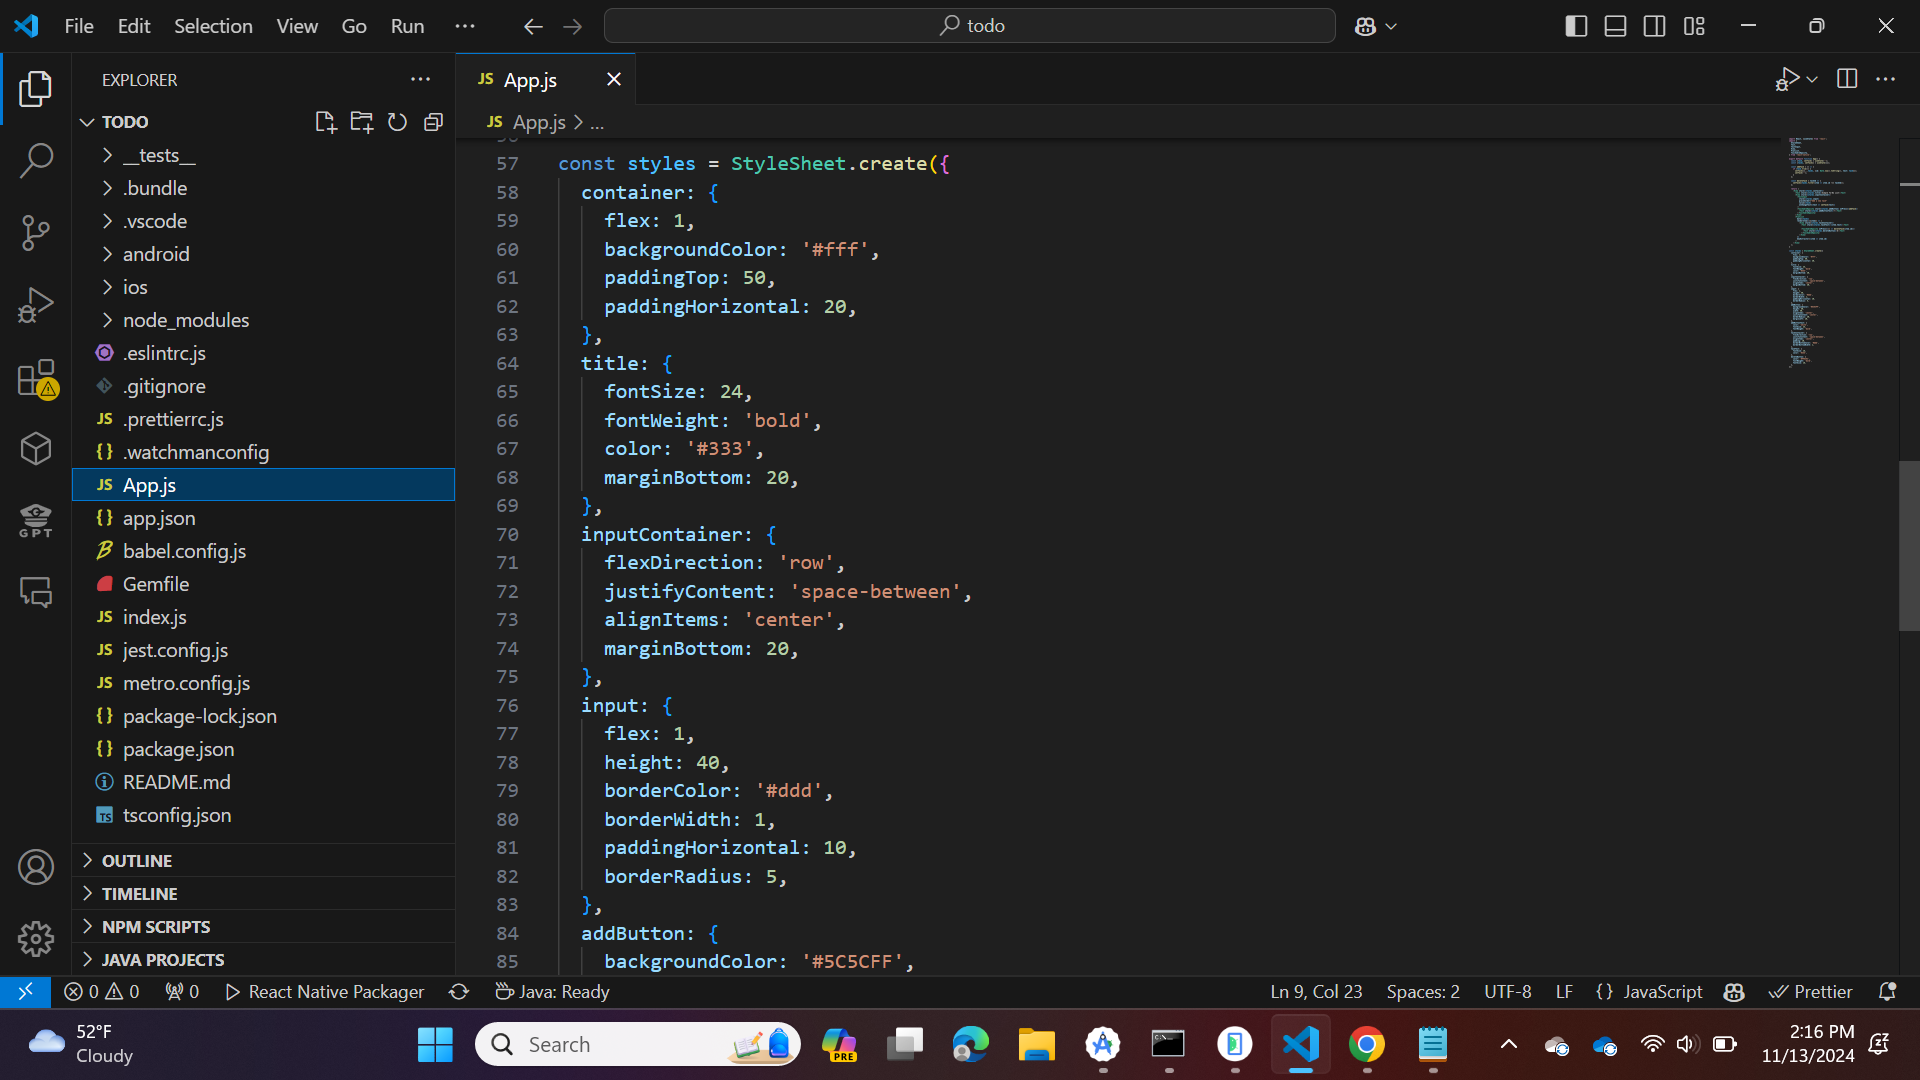
\includegraphics[width=5.57813in,height=3.13391in]{media/image37.png}

\subsection*{Step 4: Running the App}

\begin{itemize}
    \item Run the app with:
    \begin{lstlisting}[language=bash]
    npx react-native run-android
    \end{lstlisting}
\end{itemize}
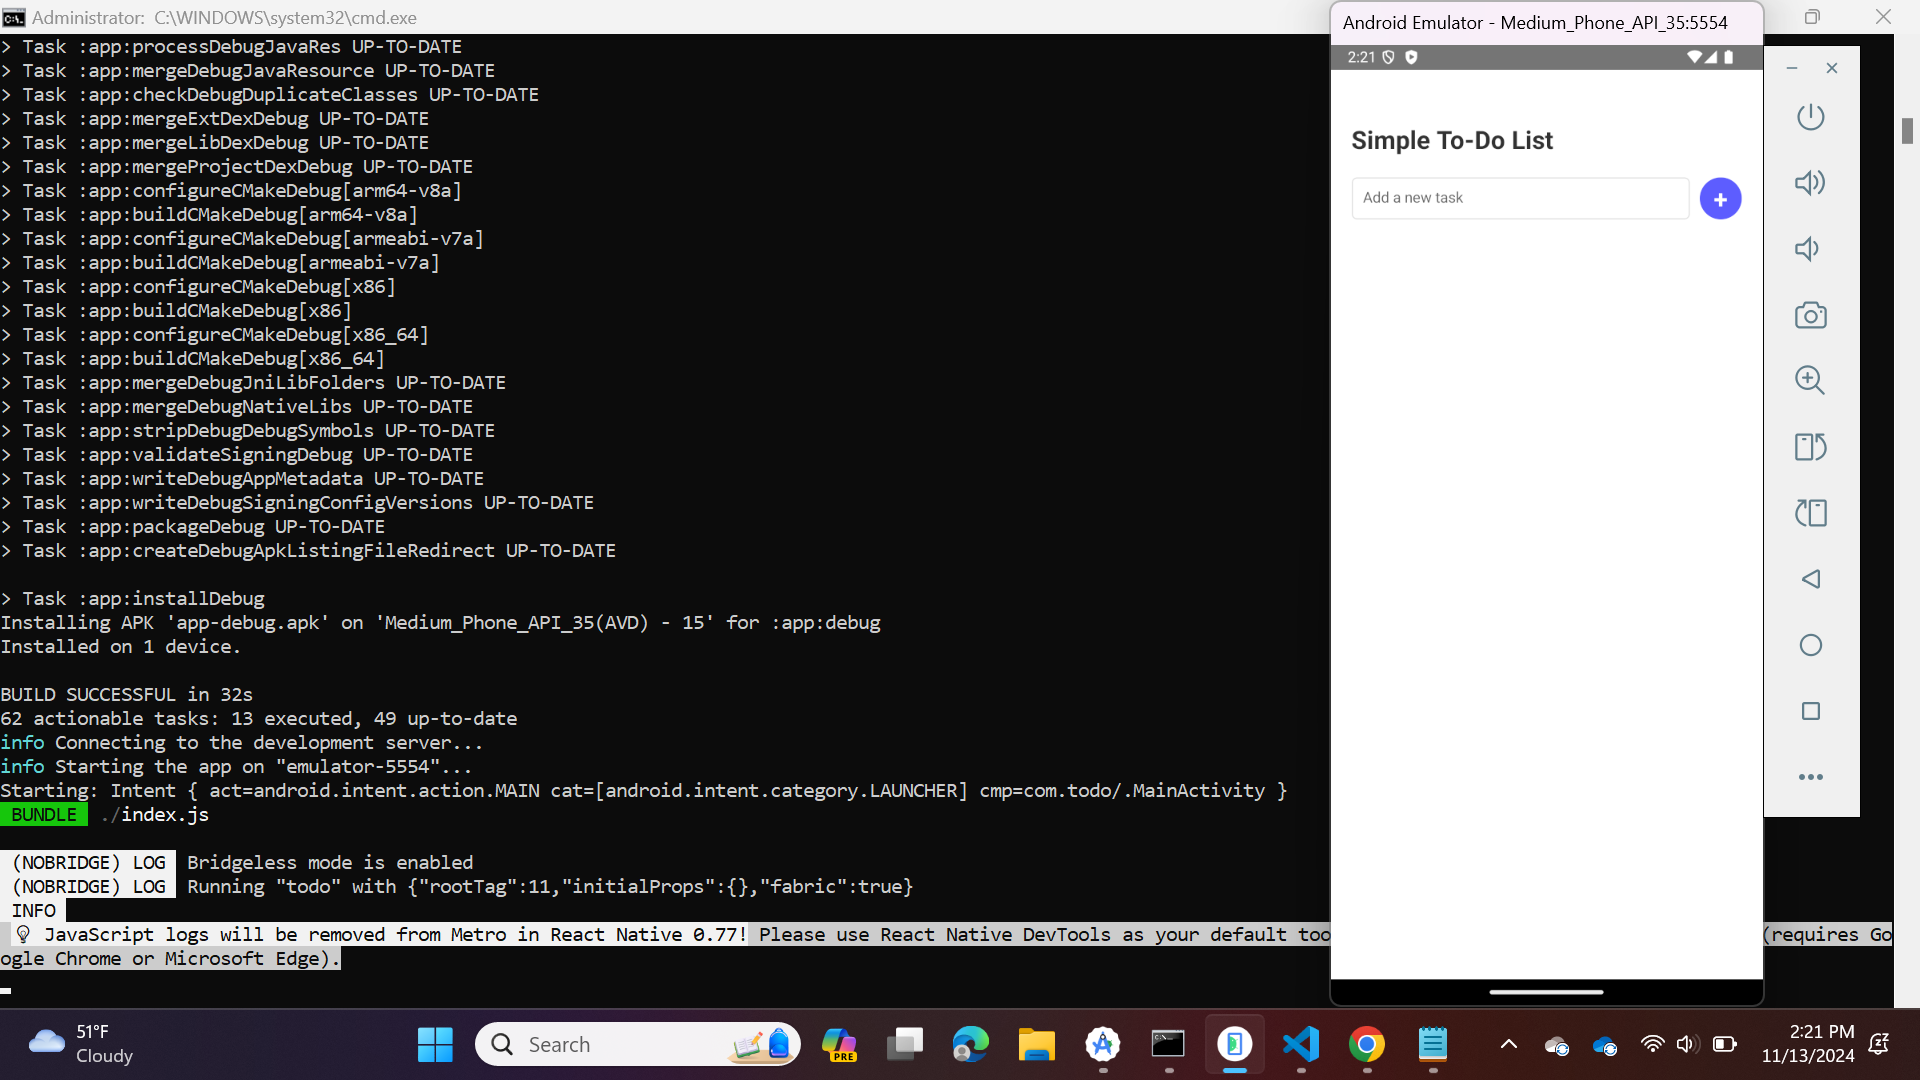
\includegraphics[width=5.57813in,height=3.13391in]{media/image16.png}

\begin{itemize}
    \item This compiles and launches the app on your selected platform.
\end{itemize}

\section*{Features to Implement}

\begin{enumerate}
    \item \textbf{Mark Tasks as Complete (15 Points):}
    \begin{itemize}
        \item Add a toggle function to mark tasks as completed.
        \item Style completed tasks with strikethrough text or color changes.
    \end{itemize}
\end{enumerate}
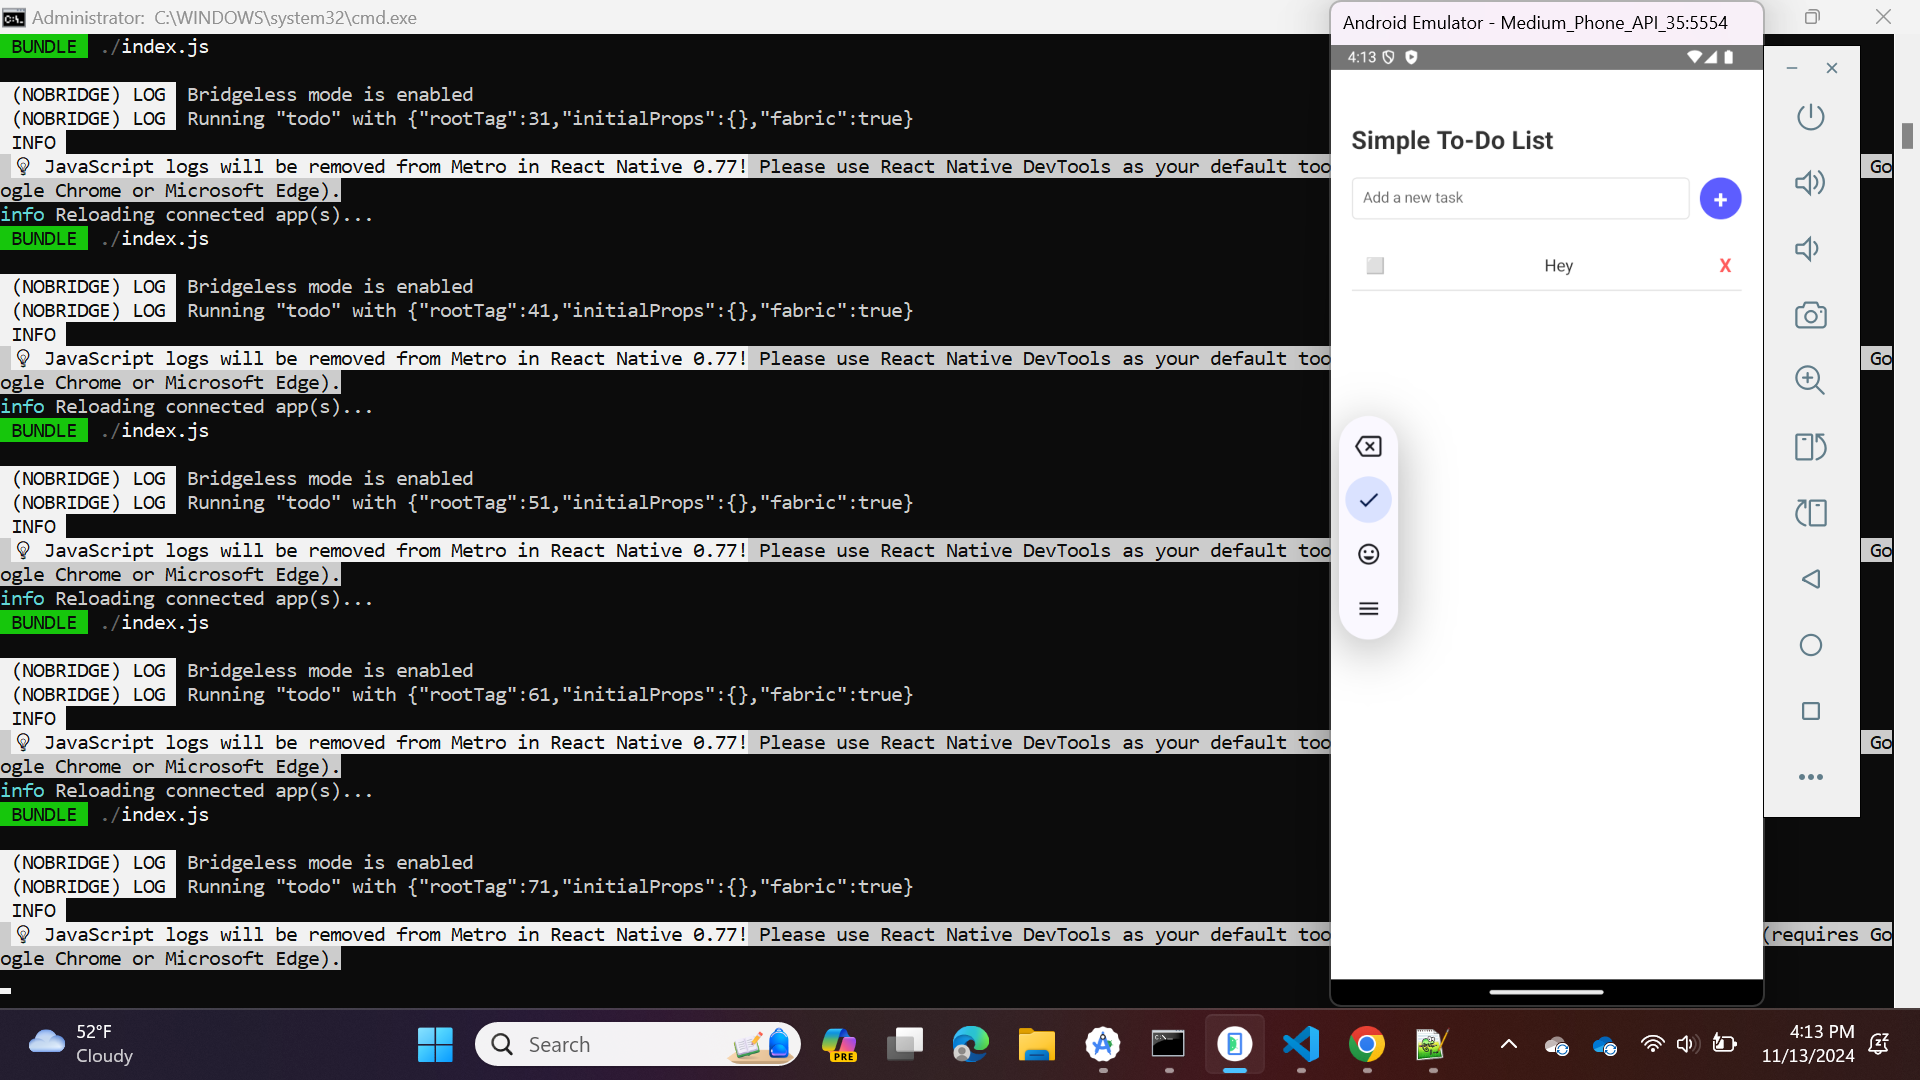
\includegraphics[width=5.57813in,height=3.13391in]{media/image34.png}
    
\begin{enumerate}
    \item \textbf{Persist Data Using AsyncStorage (15 Points):}
    \begin{itemize}
        \item Use AsyncStorage to save and retrieve tasks, ensuring persistence after app closure.
    \end{itemize}
\end{enumerate}
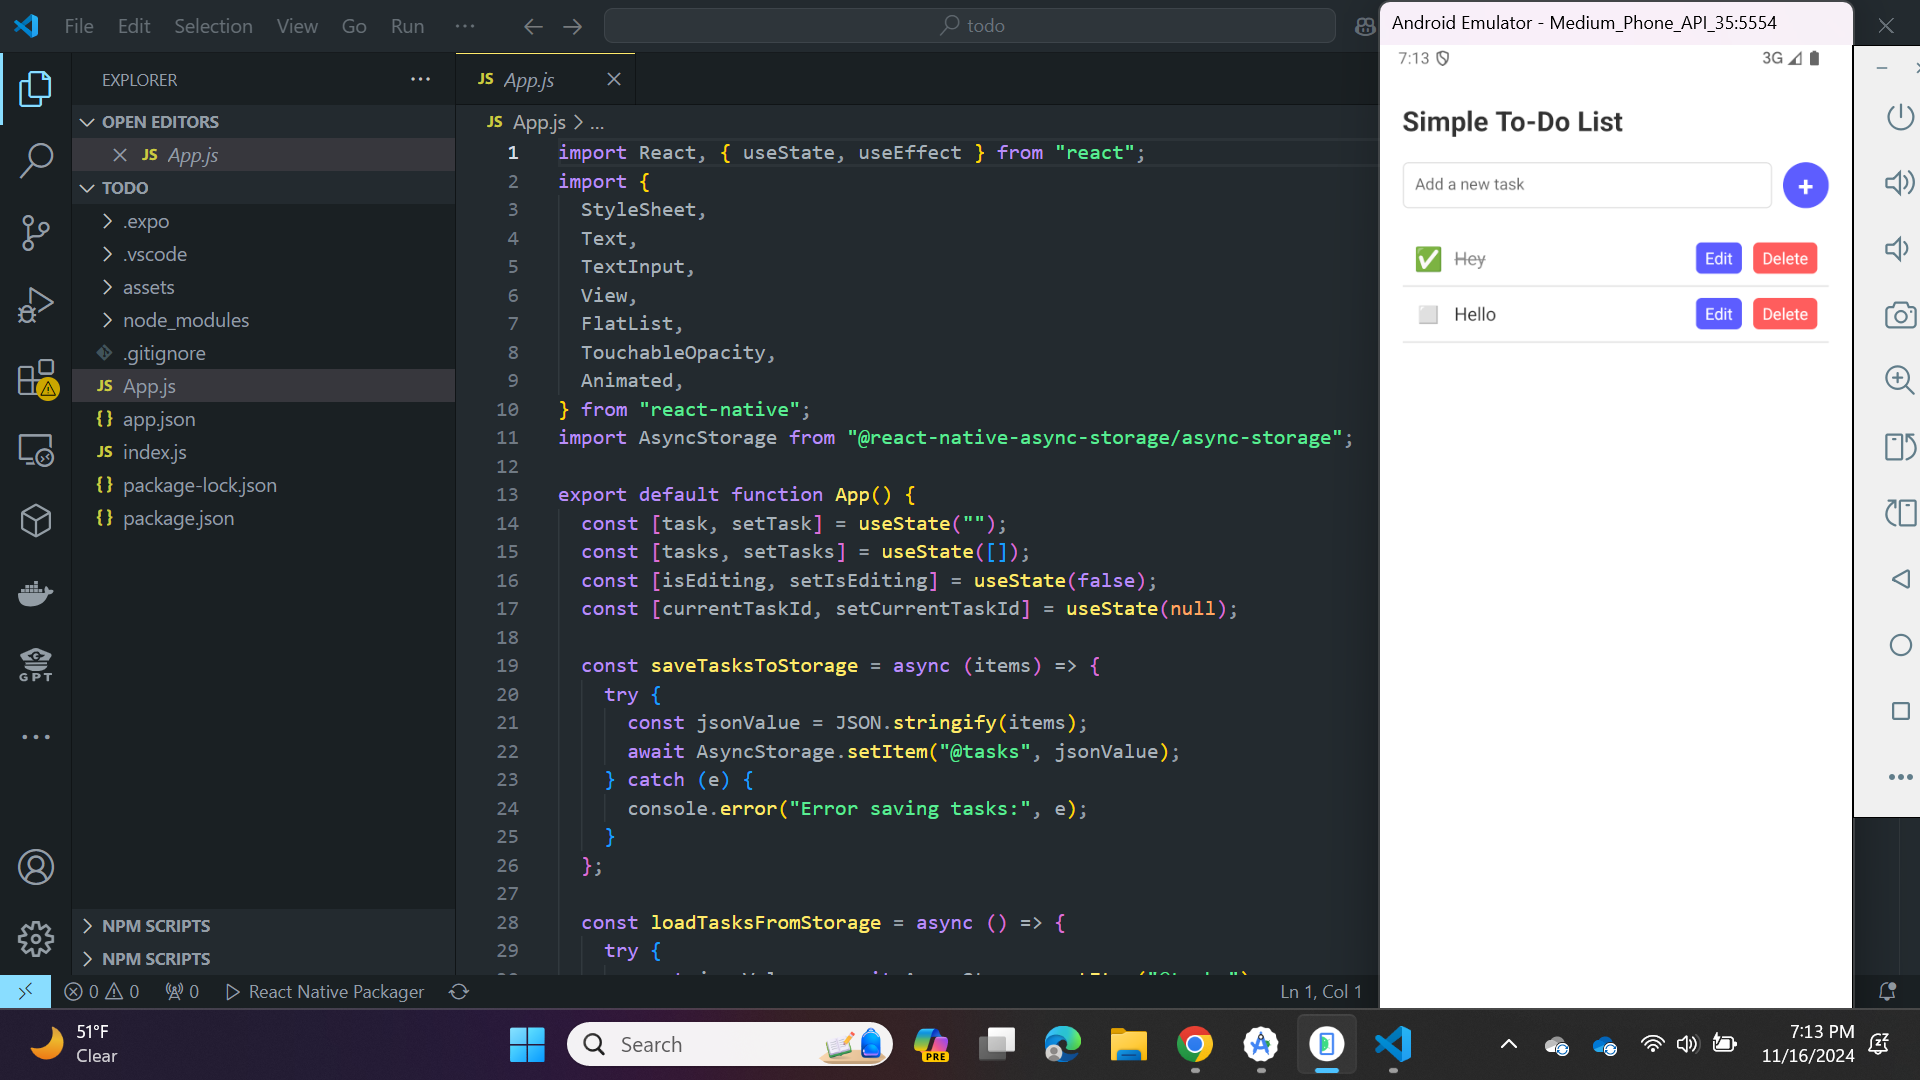
\includegraphics[width=5.57813in,height=3.13391in]{media/image23.png}

\begin{enumerate}
    \item \textbf{Edit Tasks (10 Points):}
    \begin{itemize}
        \item Allow users to tap on tasks to edit their content.
        \item Implement a function to update tasks in the state array.
    \end{itemize}
\end{enumerate}
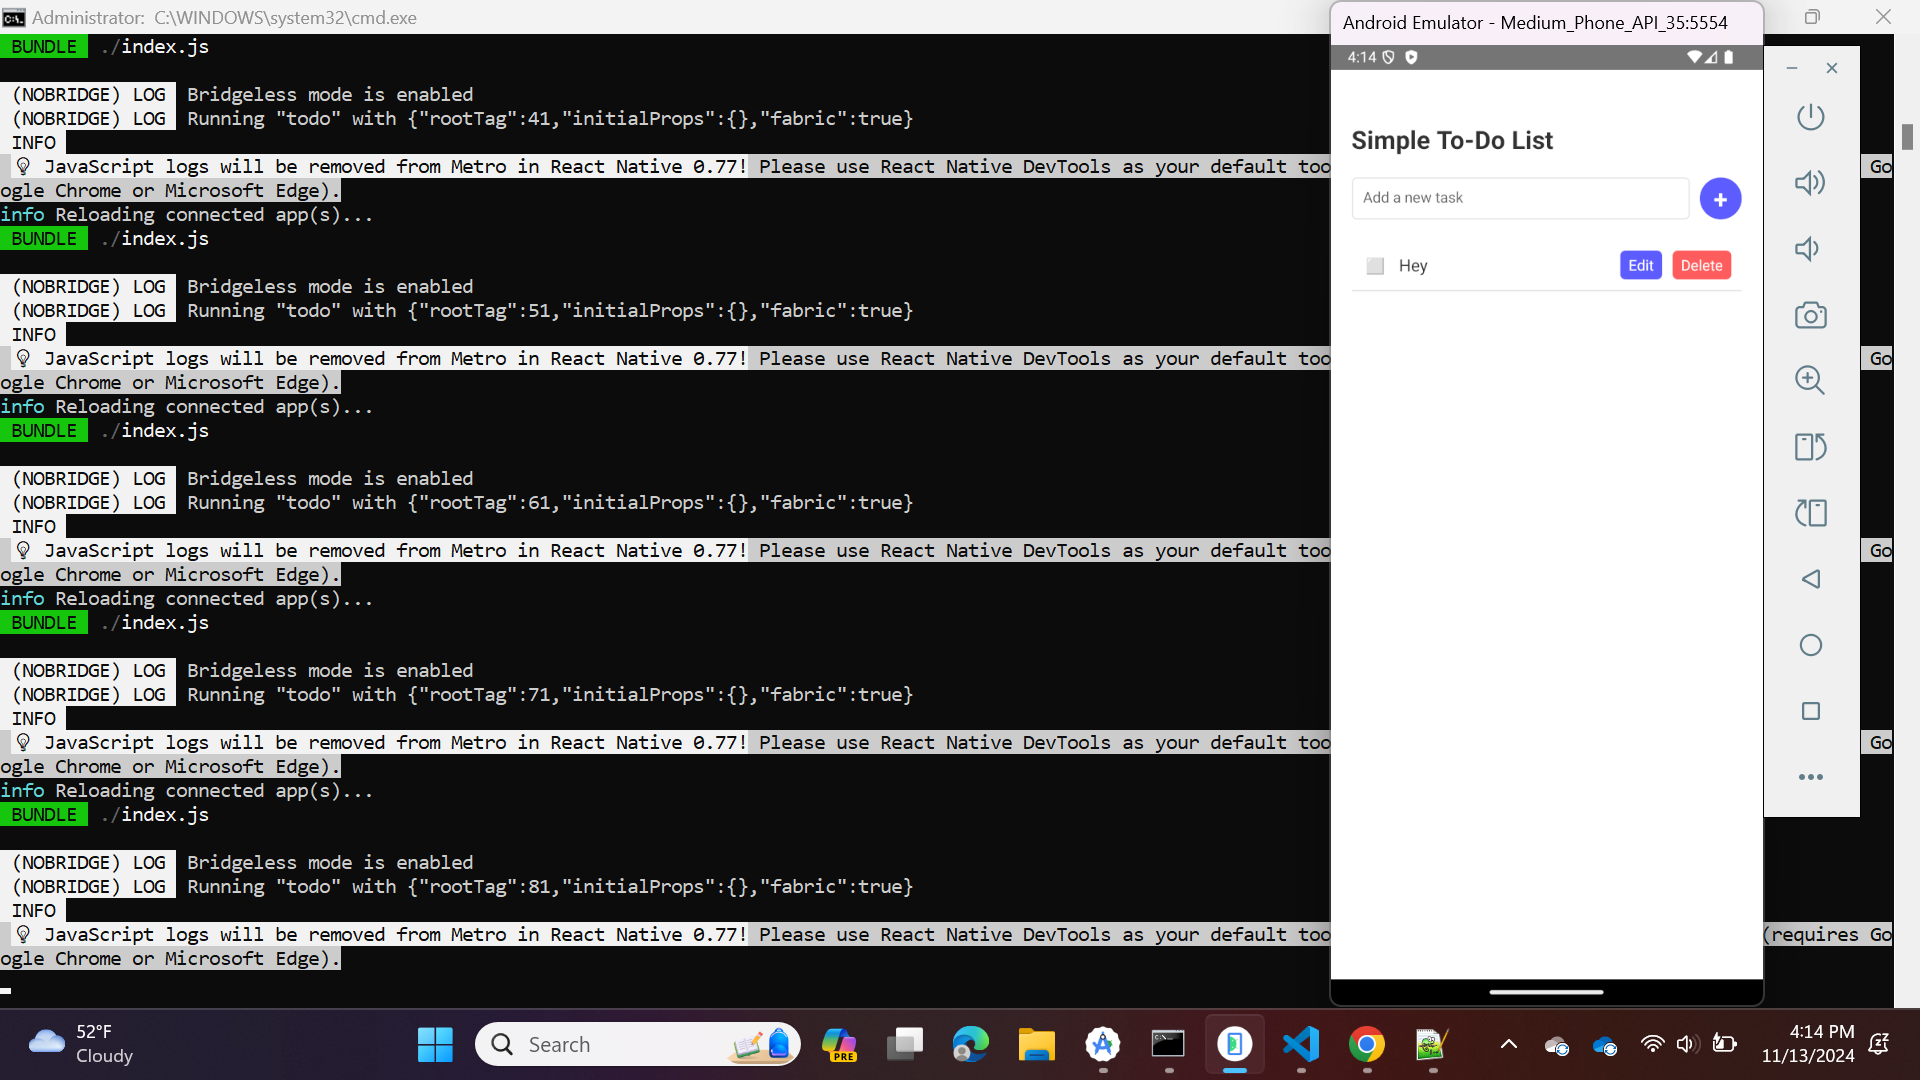
\includegraphics[width=5.57813in,height=3.13391in]{media/image11.png}

\begin{enumerate}
    \item \textbf{Add Animations (10 Points):}
    \begin{itemize}
        \item Use the Animated API for visual effects when adding or deleting tasks.
        \item Describe how animations enhance the user experience.
    \end{itemize}
\end{enumerate}
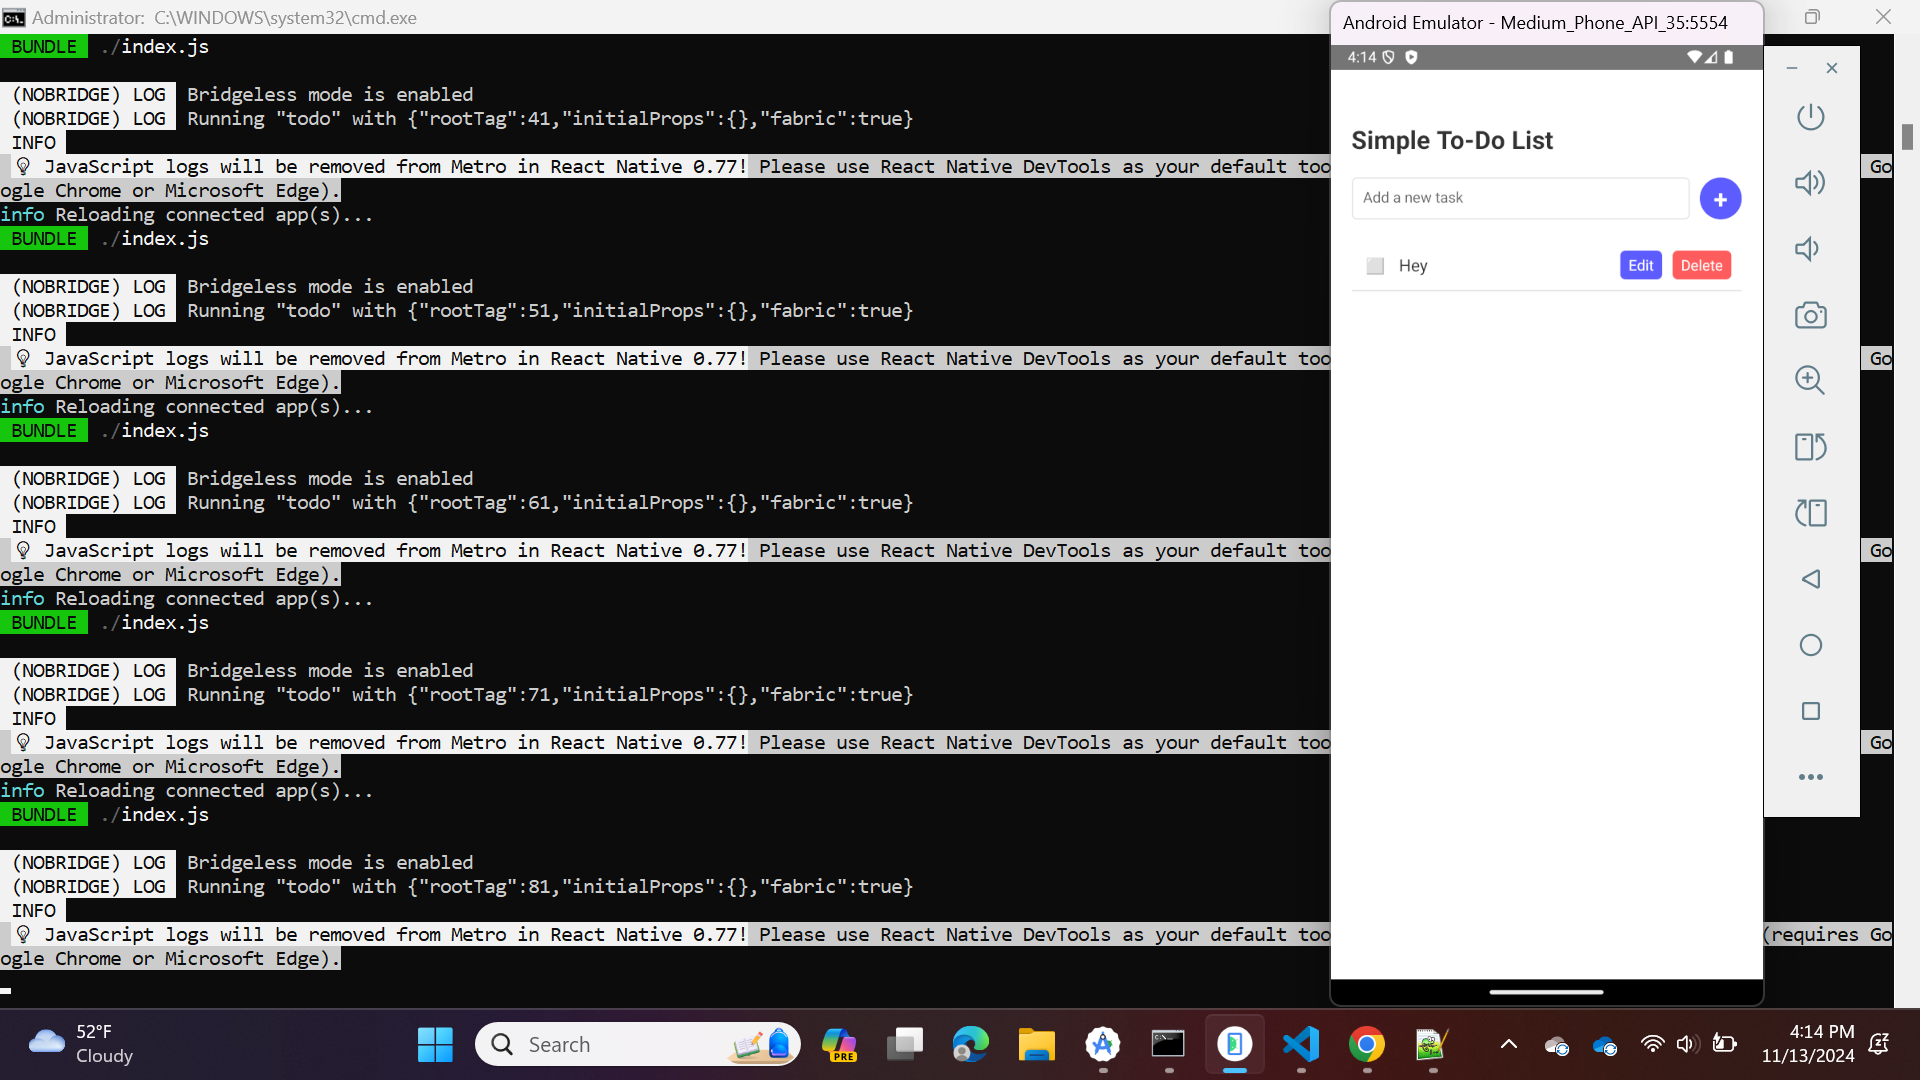
\includegraphics[width=5.57813in,height=3.13391in]{media/image11.png}

\begin{itemize}
    \item Changed UI Styling:   
\end{itemize}
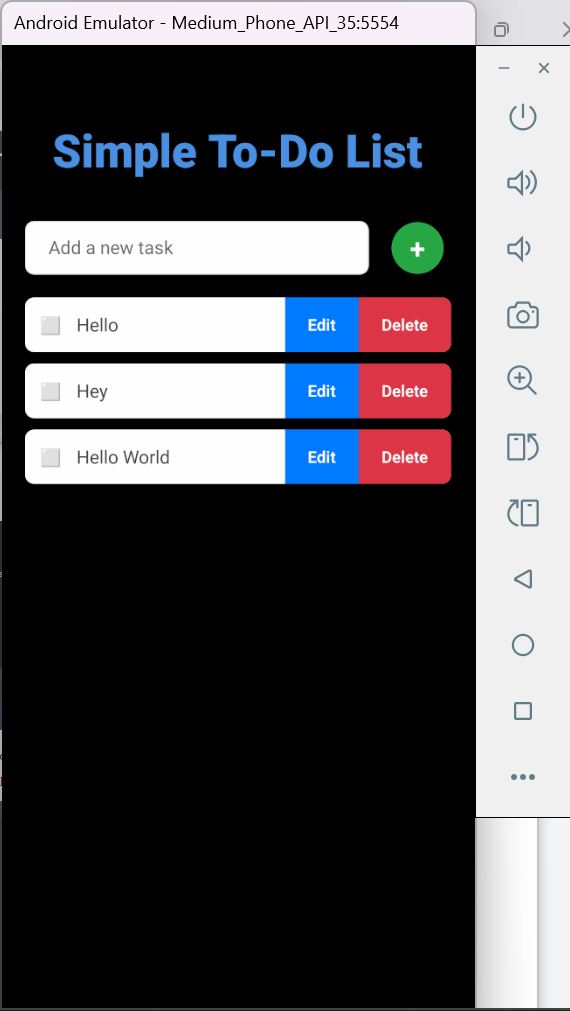
\includegraphics[width=3.14063in,height=5.53233in]{media/image38.png}
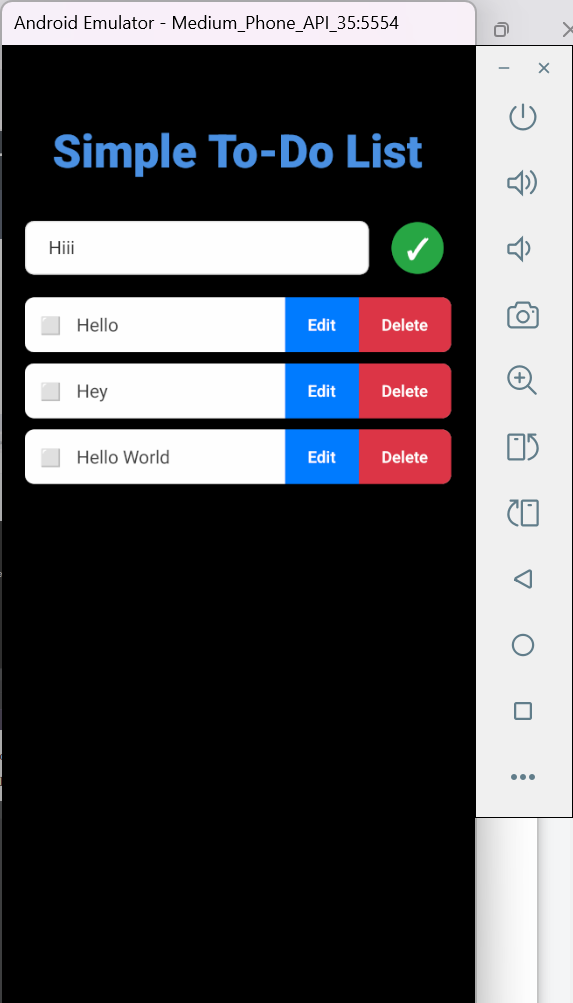
\includegraphics[width=3.14063in,height=5.53233in]{media/image39.png}
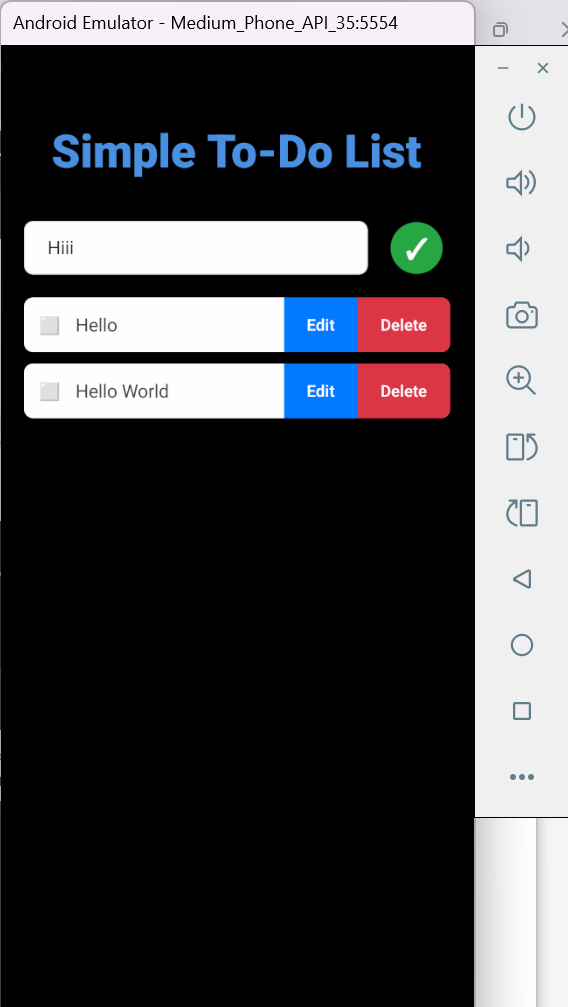
\includegraphics[width=3.14063in,height=5.53233in]{media/image40.png}
    

\end{document}
